\documentclass[preprint]{sig-alternate-05-2015}

\usepackage{url}                  % format URLs
\usepackage{listings}          % format code
\usepackage{enumitem}      % adjust spacing in enums
\usepackage{hyperref}
\usepackage{amsmath}
\usepackage{amssymb}
\usepackage{tikz}
\usetikzlibrary{arrows,%
                shapes,positioning}

\usetikzlibrary{calc}


\newtheorem{definition}{Definition}
\newtheorem{proposition}{Proposition}
\newtheorem{corollary}{Corollary}
\newtheorem{theorem}{Theorem}
\newtheorem{remark}{Remark}
\newtheorem{example}{Example}
\def\qed{{\hfill\rule{1.2ex}{1.2ex}}}
%\newenvironment{proof}{{\em{Proof: }}}{\qed}

% -------New
\def\Vp{{\tt{Varsp}}}
\def\Vd{{\tt{Varsd}}}
\def\Stmtp{{\tt{Stmtp}}}
\def\Stmtd{{\tt{Stmtd}}}
\def\psp{{\tt{PSp}}}
\def\psd{{\tt{PSd}}}
\def\semp{{\tt{Semp}}}
\def\semd{{\tt{Semd}}}
% -------New

\newcommand\ignore[1]{{}}
\def\sender{{\tt{Sender}}}
\def\chooser{{\tt{Chooser}}}
\def\UndefV{{\tt{InputV}}}
\def\DefV{{\tt{DefV}}}
\def\zero{{\tt{zero}}}
\def\float{{\tt{float}}}
\def\int{{\tt{int}}}
\def\vmap{{\tt{vmap}}}
\def\ds{{\mathit{\theta}}}   % dual state
% \def\dps{{\tt{DPS}}}      % set of all dual states
%\def\Vt{{\tt{VarsB}}}
\def\domp{{\tt{Domp}}}
\def\domd{{\tt{Domd}}}
\def\doma{{\tt{Doma}}}
\def\paths{{\tt{Paths}}}
%\def\pps{{\tt{PPS}}}
%\def\Stmt{{\tt{Stmt}}}
\def\assume{{\tt{assume}}}
%\def\dom{{\tt{Dom}}}
%\def\int{{\tt{Int}}}
%\def\domt{{\tt{Typ}}}
%\def\intt{{\tt{TCC}}}
%\def\domt{{\tt{DomB}}}
%\def\intt{{\tt{IntB}}}
\def\spec{{\tt{spec}}}
\def\fspec{\phi_{\tt{fspec}}}
\def\nfspec{\phi_{\tt{nfspec}}}
\def\Sig{{\Sigma}}
\def\V{{\tt{Vars}}}
\def\Tau{{\tt{Terms}}}
%\def\sem{{\tt{Sem}}}
%\def\semt{{\tt{SemB}}}

\def\true{{\mathit{true}}}
\def\false{{\mathit{false}}}

%\def\ctxt{{\mathit{ctxt}}}
%\def\top{{\mathtt{top}}}
%\def\uses{{\mathtt{uses}}}

\def\ZZ{{\mathbb{Z}}}
\def\Float{{\mathbb{Q}}}
\def\RR{{\mathbb{R}}}
\def\zero{{\mathtt{zero}}}
\def\integers{{\mathtt{int}}}
\def\floats{{\mathtt{float}}}
\def\assert{{\mathtt{assertp}}}
\def\assertt{{\mathtt{assertd}}}

\def\Stack{{\mathtt{Stack}}}
\def\vals{{\mathtt{Vals}}}
\def\ite{{\texttt{if-then-else}}}

\def\nreach{{\mathtt{nreach}}}
\def\MMul{{\mathtt{Mul}}}
\def\VAdd{{\mathtt{Add}}}
\def\conv{{\mathtt{conv}}}
\def\scales{{\mathtt{scales}}}
\def\homo{{\mathtt{homo}}}
\def\cnst{{\mathtt{cnst}}}
\def\attr{{\mathtt{attr}}}

\def\iteif{{\mathit{if}}}
\def\itethen{{\mathit{then}}}
\def\iteelse{{\mathit{else}}}
\def\itefi{{\mathit{if}}}
\def\while{{\mathit{while}}}

\def\lfp{{\mathtt{lfp}}}
\def\gfp{{\mathtt{gfp}}}
\def\push{{\mathit{push}}}
\def\pop{{\mathit{pop}}}

\def\bnfalt{{\;\;{\mid}\;\;}}
\def\bnfis{{\;\;::==\;\;}}

\begin{document}

\special{papersize=8.5in,11in}
\setlength{\pdfpageheight}{\paperheight}
\setlength{\pdfpagewidth}{\paperwidth}

\setcopyright{acmcopyright}
%\copyrightyear{20yy}
\doi{nnnnnnn.nnnnnnn}
\isbn{978-1-nnnn-nnnn-n/yy/mm}
\conferenceinfo{CONF 'yy}{Month d--d, 20yy, City, ST, Country}

% Uncomment the publication rights you want to use.
%\publicationrights{transferred}
%\publicationrights{licensed}     % this is the default
%\publicationrights{author-pays}

%\titlebanner{}        % These are ignored unless
%\preprintfooter{}   % 'preprint' option specified.

%\title{Bounded Program Synthesis}
\title{Search for Proof to Search for Programs: Duality for Bounded Program Synthesis}

\numberofauthors{1}
\author{
\alignauthor
Firstname Lastname\\
\affaddr{Affiliation1}\\
\affaddr{Affiliation2}\\
\email{email@address}
}
%\author{Adri{\`a} Gasc{\'o}n} \and Ashish Tiwari \and Brent Carmer \and Umang Mathur}
%\authorrunning{A. Tiwari \and B. Carmer \and A. Gascon}
%\institute{ SRI International, Menlo Park, CA 94025 } 
% {\{tiwari,gascon,bcarmer\}@csl.sri.com}

\maketitle

\begin{abstract}
We introduce a technique for program synthesis that
is based on searching for the proof of correctness
of the target program, rather than searching for the 
correct program directly.
Our technique, which we call bounded synthesis,
relies on a proof system that checks the correctness
property of the target program, and searches for
a proof in that proof system. Our approach is based
on a notion of duality that reduces safety verification
to constraint solving. 
% The program can then be
% read off from the discovered proof.

A significant benefit of the approach is that it can
uniformly handle both functional and non-functional
criteria for correctness.
A distinctive feature of
bounded program synthesis is that
it solves synthesis problem by generating an
$\exists\exists$ constraint, whereas traditional program
synthesis approaches are based on solving an
$\exists\forall$ constraint.
We use bounded program synthesis to
automatically synthesize several intricate and
non-obvious cryptographic constructions.
%
% We define the notion of primal and dual components
% of programs.  Whereas primal components have the
% standard meaning of a program, dual components 
% define constraints, or rules, that must not be
% violated in an accepted execution.
% The dual components may not be necessarily related to 
% the primal, and can be used to capture nonfunctional
% correctness properties of programs. 
%
% In some cases, it is possible to design a dual
% component that subsumes the correctness criteria
% stated using a primal. This gives us
% a duality principle.  We apply duality to program
% synthesis to convert a problem that is 
% traditionally solved as an 
% $\exists\forall$ problem to an
% $\exists\exists$ problem.
%One of its most striking manifestations is in the
%theory of linear arithmetic, which gives rise
%to several results in the field of linear programming.
%One such example is the Farkas' lemma, which converts
%validity of universal (arithmetic) formulas to
%satisfiability (and *not* unsatisfiability)
%of existential (arithmetic) formulas.
%
%We present a similar duality principle in
%program analysis.
%
%We use duality to introduce Synudic -- a language
%for program synthesis. Synudic allows synthesis of straight-line
%programs using the Yices Exists-Forall (EF) solver. However, and more
%importantly, thanks to duality, synthesis may sometimes require
%only the Yices SMT solver (and *not* the EF solver).
\end{abstract}

%\category{CR-number}{subcategory}{third-level}

% general terms are not compulsory anymore,
% you may leave them out
%\terms
%term1, term2

\keywords
synthesis, syntax-guided synthesis, bounded proof search, abstract interpretation, duality

%\author{Ashish Tiwari \and Brent Carmer \and Adri{\`a} Gasc{\'o}n}
%\authorrunning{A. Tiwari \and B. Carmer \and A. Gascon}
%\institute{ SRI International, Menlo Park, CA 94025 } 
% {\{tiwari,gascon,bcarmer\}@csl.sri.com}


\section{Introduction}
\label{sec:intro}

Duality is a central concept in Mathematics and Computer Science.
One of its most striking manifestations is in the
theory of linear arithmetic, which leads to 
several important insights and computational techniques
in the field of linear programming.
In this paper, we present a duality principle for program analysis
and show how it can be used to improve automatic program synthesis
techniques.

For a rather simple intuition about duality in linear arithmetic, 
consider the problem of deciding
validity of a universal formula in linear rational arithmetic (LRA).
For example, a concrete instance would be the formula
$$
 \forall{x,y}: x+y\geq 0\wedge x-y\geq 0 \Rightarrow x+1 \geq 0
$$
If a universal formula is not valid, then there is a witness -- namely,
a concrete value for the quantified variables ($x$ and $y$ in the 
example formula) -- that can be used to efficiently (in polynomial time)
demonstrate the invalidity. 
In other words, % we are just stating that 
validity of forall formulas
in LRA is in co-NP.

Consider, now, the satisfiability problem of an existentially
quantified LRA formula.
If such an existential formula is satisfiable, then there is a witness -- 
namely, a concrete value for the quantified variables -- that can be used 
to efficiently (in polynomial time) demonstrate that the formula
is satisfiable. 
In other words, % we are just stating that 
satisfiability of existential formulas
in LRA is in NP.

The duality principle in linear arithmetic allows us to transform
the validity problem (a co-NP problem) to satisfiability of an existential
formula  (a NP problem). 
Duality shows that we have a small witness for such problems
in both the ``yes'' and ``no'' answers and hence, these problems
are in NP and co-NP. (In fact, we know that they are in P.)
The intuition behind obtaining the {\em{dual}} satisfiability problem from
the original validity problem is as follows: 
the facts 
 $x+y\geq 0$ and $x-y\geq 0$ will imply $x+1 \geq 0$ iff
$x+1$ can be written as a positive linear combination of $x+y$, $x-y$ and $1$.
More generally, given a validity problem, the {\em{dual}} satisfiability problem is 
obtained by introducing a dual variable for each atomic formula
(Lagrange multiplier) and one dual variable for the hidden atomic formula $1 > 0$.
For the above concrete example, we get the following dual problem:
$$
 \exists{u,v,w}: u+v=1 \wedge u-v = 0 \wedge w=1 \wedge u,v,w \geq 0 
$$
The formula above is saying that we can get $x+1$ by multiplying $x+y$ by $u$,
$x-y$ by $v$ and $1$ by $w$, where $u,v,w$ are all non-negative.
Indeed, the original forall formula is valid and the dual existential formula
is satisfiable.

Duality has allowed us to trade a $\forall$ quantifier with an $\exists$ quantifier
{\em{without}} changing (or negating) the answer. 
As one can imagine, such a duality result is a very strong result, and we can not
expect to have answer preserving quantifier replacement for more complex problems.
For example, if we had a such a result for Boolean logic, then (assuming the 
quantifier exchange does not blow up the formula) the polynomial hierarchy would
collapse as quantified Boolean satisfiability would become equivalent to 
just Boolean satisfiability.
Nevertheless, we can have weaker forms of duality, where we have answer preservation
in only {\em{one direction}}. In other words, from a $\forall$ problem, we may be
able to generate an $\exists$ problem such that a ``yes'' answer for the
$\exists$ problem implies a ``yes'' answer for $\forall$ problem, but not
necessarily vice-versa.  This weaker form of duality is pervasive in program
analysis, % and we formalize it in this paper, 
and we use it in this paper to obtain an
effective and promising way to solve (certain class of) program synthesis problems.

% Programs consist of two kinds of entities: values and types.
%Values are manipulated during program executions, and
%users can program these manipulations in a flexible way. For
%example, users can define new functions and compose these
%functions to define more complex value manipulation routines.
%This is not the case for the other entity, namely types.
%Programming languages usually have a predefined set of base
%types, and even though a user can build more complex types,
%such as records, arrays, and lists, using the base types,
%there is still less flexibility available than for values;
%for example, a user typically cannot define rules (programs)
%for the manipulation of types.
%
%We envision here a language where users could define and manipulate
%type-like entities in conjunction with regular values.
%What would be the behavior of such programs?
\ignore{
It has been pointed out
by Cousot~\cite{Cousot97} that there is a certain {\em{duality}}
between values and types:
specifically, there is a Galois connection between
properties (on values) and types where, for example,
set union in one lattice corresponds to set intersection in the other.
More intuitively and less formally, a variable
that has {\em{more}} types can take on {\em{fewer}} values
and vice versa. For example, a variable that has types
${\mathtt{even}}$
and ${\mathtt{pos\_int}}$ (union of types)
% can it takes {\em{fewer}} values: in this example,
can only be a positive even integer (intersection on values).
\endignore}

%What does this mean if we were to have a program that
%allowed computation on type-like entities?
%We would need to perform {\em{dual}} operations:
%rather than union at control flow join points
%(that we do for values),
%we would perform intersection, and
%rather than least fixpoint computation in loops
%(that we do for values),
%we would perform greatest fixpoit computation.
%We would like to have programs that, semantically,
%perform unions at control flow join points for
%certain values, and that simultaneously, semantically, perform
%intersection at control flow join points for certain
%other ``type'' values.

\ignore{
In the usual notion of types, we have types
representing a set of concrete values.
We wish to go beyond this standard notion and
consider arbitrary user-defined entities that
behave like types, but that are not necessarily
related in any way to the concrete semantics of the program.
Let us call this more general notion {\em{dual values}}.
So, a program variable will be mapped to not only a value,
as in the usual semantics of programs, but also
simultaneously to a dual value.
Moreover, as in the case of types, 
this dual value does not correspond to
the result of a particular execution, 
but to a property that holds in every execution.
A user can not only program how values are updated
in a program, but also program the rules that govern
the update of dual values. 

%Thus, we achieve our goal
%of programming with primal and dual semantics.
%
The obvious question to ask here is why should one be
interested in programmable dual values and the dual
semantics that govern their behavior.
There are three main reasons:
(1) it provides a framework for using types-like 
constraints to prune search space in 
program synthesis, (2) it enables specification of
nonfunctional properties, and (3) it provides a new
way to think about program analysis and synthesis,
and helps provide theoretical clarity in that space.

\endignore}

Our contributions are as follows:
\begin{itemize}\itemsep=0em
    \item We  introduce {\em{bounded program synthesis}}, where
    a bounded search for proof in a given proof system 
    is used as an approach to synthesize correct programs.
  \item We show that bounded proof search can be used to
    either augment an (exists-forall) synthesis constraint, or 
    entirely replace it by an exists-exists constraint.  
    We identify a {\em{weak duality}} principle, which
    enables replacement of a forall check
    (program is correct for all inputs)
    by an exists check (there exists a proof),
    and thus allows us to perform
    synthesis by solving an exists-exists constraint.
  \item We show that standard abstraction techniques provide one
    way of generating proof systems on which bounded proof
    search can be performed. Bounded proof search is performed by 
    paramterizing
    the elements of the abstract domain (as in template-based
    program verification), and then 
    finding values for these parameters that correspond to valid
    application of the proof rules (exists constraint).
  \item We demonstrate that the security is an ideal
    domain for application of automated program synthesis technology,
    thus, solidifying preliminary evidence in this 
    regard~\cite{zoocrypt,DBLP:conf/csfw/MalozemoffKG14,TGD15:CADE,KatzBestPaper,BrentNew}.
    The bounded proof search using dual interpretations introduced here 
    eases the task of specifying security requirements.
\end{itemize}

We start by introducing a programming formalism that admits
both primal and dual (program) variables 
and present the distinction between
the two at an abstract semantic level (Section~\ref{sec:language}).
We then present a duality result (Section~\ref{sec:duality}),
show how it can be used to perform program synthesis (Section~\ref{sec:synthesis}),
and finally show its application 
to synthesis of cryptographic schemes (Section~\ref{sec:application}).


\ignore{

\begin{description}
  \item[Using types in program synthesis.]
    One motivation comes from the field of
    program synthesis. Suppose we are interested in
    synthesizing a 10 line program that meets some
    specification. Even for a relatively small
    expression language, the number of 10 line programs
    that can be constructed using that language will
    be huge. However, the number of well-typed programs
    could be significantly smaller. This point was also
    made in recent work on synthesis of functional
    programs~\cite{DBLP:conf/pldi/OseraZ15}.
    So, how to impose type constraints on a yet-to-be
    synthesized program?
    If $x := f(y)$ is the form of assignment statement
    on line~3, where $f$ is some {\em{unknown}} function
    symbol that is chosen from the expression language,
    then {\em{a priori}} we do not know the types of $x$
    and $y$. However, if every value variable $x$ can
    carry with it a dual value,
    then we encode typing constraints
    on the program by constraining the dual values.
    As a result, when solving the synthesis problem, we now
    synthesize both the program and a type correct annotation
    for it.
    Thus, we can use dual values and dual semantics to impose
    typing constraints on ``program sketches'' and 
    help prune the search space of possible programs.
    This is discussed further in Section~\ref{sec:synthesis}.

  \item[Nonfunctional program properties.]
    Since programs are assigned one concrete semantics that
    specifies the functional behavior of the program,
    we can easily state properties that relate to
    {\em{functional correctness}} of programs.
    Moreover, by using abstractions of the concrete
    semantics~\cite{CousotCousot77:POPL}, we can reason about
    programs and perhaps prove functional correctness.
    However, increasingly we are getting interested in
    {\em{nonfunctional properties}} of programs -- properties
    of programs that are not directly related to its concrete semantics.
    One example class of nonfunctional properties
    consists of properties related to security, such as
    secure information flow~\cite{DBLP:journals/cacm/DenningD77}.
    Since these are nonfunctional properties, it is then
    no surprise that dedicated ``type systems'' that are unrelated
    to the concrete semantics are
    developed
    for reasoning about them~\cite{DBLP:conf/csfw/Smith01,DBLP:conf/csfw/MalozemoffKG14}.
    The development of dual semantics
    can enable programming of such nonstandard type systems in a
    general-purpose language, and potentially increase
    utility of programming languages in general.

    % Switching from verification to synthesis in this context,
    % we note the recent work on synthesis of security schemes
    % using program synthesis techniques~\cite{TGD15:CADE}, where security
    % requirements are captured in a second interpretation
    % that supplements the primary intrepretation, which itself
    % is used to specify functional requirements.


  \item[Theoretical interest.]
    Our work is also motivated by theoretical interest in
    identifying the appropriate notion of
    dual semantics and the duality principle in program analysis.
    In particular, we note an asymmetry in the complexity
    of assertion checking for imperative programs:
    for a polynomial time (PTime) program, the problem of
    checking if an assertion is valid is in co-NP.
    % if the assertion is {\em{violated}}, then there is some
    % input that causes assertion failure, and hence one could
    % (nondeterministically) guess that input and check
    % that the assertion is violated in PTime.
    For the same program, under reasonable assumptions,
    checking if an assertion on the dual semantics is valid
    happens to be in NP.
    % we just need to guess the attribute
    % for each variable and check that the guesses satisfy the
    % rules defining the dual semantics.
    Furthermore, in some cases, one can design a dual semantics such
    that requirements on the dual subsume requirements specified in 
    the primal semantics.
    For program analysis, this means we replace a ``search for bugs''
    (violation of primal requirements)
    by a ``search for proofs'' (satisfiability of dual requirements).
    This is discussed further in Section~\ref{sec:assertionchecking}
    and Section~\ref{sec:duality}.


\end{description}

\endignore}

\ignore{
\subsection{Outline}

We present primal and dual semantics for imperative
programs constructed using a very simple
programming language. The language is presented in
Section~\ref{sec:language}.
We present the semantics in stages. First, we present
it for straight-line programs
(Section~\ref{sec:straightline}), and then
for loop-free programs
(Section~\ref{sec:loopfree})
and finally for
programs with loops
(Section~\ref{sec:loops}).
In each of the three sections corresponding to the three
stages, we will start with an example that will provide
motivation and intuition for the definitions that follow.
We discuss the application of dual semantics to
program synthesis in Section~\ref{sec:synthesis}.
%We envision programs

\endignore}

%\section{Illustrating Primal and Dual Programs}
%In this section, we provide some simple examples that illustrate
%the definitions and developments in the rest of the paper.

\ignore{ %% different formalization of programs -- as a graph now

\begin{figure}[t]
\begin{center}
\[
  \begin{array}{rcll}
    {\tt{Stmt}} & \bnfis & x := f(\vec{x})
             \\ & \bnfalt & {\iteif} (c) \;{\itethen}\; {\tt{Prgm}} \;{\iteelse} \; {\tt{Prgm}} \; {\itefi}
             \\ & \bnfalt & {\while} (c) \; \{ \; {\tt{Prgm}} \; \}
    \\
    %{\tt{Block}} & \bnfis & {\tt{Stmt}} ; \; {\tt{Block}}?
    %\\
    {\tt{Prgm}} & \bnfis & {\tt{Stmt}} ; \; {\tt{Prgm}}? % \; x = e
  \end{array}
\]
\end{center}
\caption{The syntax of our simple language: $f\in\Sig$ is a function
symbol and condition $c$ is of the form $p(\vec{x})$ where
$p\in\Sig$ is a predicate symbol.}\label{fig:language}
\end{figure}

\endignore}

\def\genx{\mbox{${\mathtt{genx}}$}}
\def\geny{\mbox{${\mathtt{geny}}$}}
\def\genr{\mbox{${\mathtt{genr}}$}}
\def\gend{\mbox{${\mathtt{genu}}$}}
\def\inputa{\mbox{${\mathtt{inputa}}$}}
\def\inputb{\mbox{${\mathtt{inputb}}$}}
\def\plus{\mbox{${\mathtt{plus}}$}}
\def\minus{\mbox{${\mathtt{minus}}$}}
\def\timess{\mbox{${\mathtt{times}}$}}
\def\identity{\mbox{${\mathtt{identity}}$}}

\section{An Illustrative Example}\label{sec:ex}

\begin{figure*}[tb]
  \begin{tabular}{|llll|}
    \hline
    Library: &
    Arity $0$: & \genx, \geny, \genr, \gend, \inputa, \inputb &
    \\ & 
    Arity $1$: &  \identity&
    \\ &
    Arity $2$: & \plus, \minus, \timess&
     \\ \hline
     Sketch: &
     block $\mathtt{C}$: & \genx, \geny, \genr, \gend, \plus(-,-), \minus(-,-), \timess(-,-) & 5 lines
     \\ &
     block $\mathtt{CA}$: & \identity$(\mathtt{C})$ & 2 lines
     \\ &
     block $\mathtt{A1}$: & \inputa & 1 line
     \\ &
     block $\mathtt{A2}$: & 
     \plus$\mathtt{( (CA,A1), (CA,A1) )}$, 
     \minus$\mathtt{( (CA,A1), (CA,A1) )}$, 
     \timess$\mathtt{( (CA,A1), (CA,A1) )}$ & 1 line
       \\ &
     block $\mathtt{AB}$: & \identity$\mathtt{(A2)}$ & 1 line
       \\ &
     block $\mathtt{CB}$: & \identity$\mathtt{(C)}$  & 2 lines
       \\ &
       block $\mathtt{B1}$: & \inputb & 1 line
       \\ &
       block $\mathtt{B2}$: & 
     \plus$\mathtt{( (CB,B1,B2,LCB), (CB,B1,B2,LCB) )}$, 
     \minus$\mathtt{( (CB,B1,B2,LCB), (CB,B1,B2,LCB) )}$, &
     \\ & &
     \timess$\mathtt{( (CB,B1,B2,LCB), (CB,B1,B2,LCB) )}$ & 3 lines
       \\ &
       block $\mathtt{BA}$: & \identity$\mathtt{(B2)}$ & 2 lines
       \\ &
       block $\mathtt{A3}$: & 
       \plus$\mathtt{( (CA,BA,A3), (CA,BA,A3) )}$, 
       \minus$\mathtt{( (CA,BA,A3), (CA,BA,A3) )}$, &
       \\ & & 
       \timess$\mathtt{( (CA,BA,A3), (CA,BA,A3) )}$ & 2 lines
       \\ &
       block $\mathtt{B3}$: & \identity$\mathtt{(B2)}$ & 1 line
     \\ 
    \hline
  \end{tabular}
  \caption{{\small{Inputs to the synthesis engine consists of the
        component library and the program sketch.  For the secure 
        multiplication example, the library has 10 components: 
        $6$ functions with arity $0$,  $1$ with arity $1$, and 
        $3$ with arity $2$.
        The sketch has $11$ straight-line program blocks:
        Alice executes code in blocks $\mathtt{A1,A2,A3}$,
        Bob executes code in blocks $\mathtt{B1,B2,B3}$, and
        Carol executes block $\mathtt{C}$. 
        Blocks $\mathtt{CA,CB}$ represent values sent by Carol to
        respectively Alice and to Bob; the same convention is used in 
        naming of blocks $\mathtt{AB,BA}$.
        The syntax $\mathtt{plus((CA,A1),(CA,A1))}$ in the
        description of block $\mathtt{A2}$ indicates that Alice
        can apply $\mathtt{plus}$ on two arguments: the first argument
        has to a value computed in block $\mathtt{CA}$ or in block 
        $\mathtt{A1}$, and the same for the second argument.
        The other choices available for Alice in $\mathtt{A1}$ are
      using the $\mathtt{minus}$ or $\mathtt{times}$ component with
      the same choices for their argument.
      Note that the syntax for writing the sketch allows a user to 
      remove choices: for example, in Block $\mathtt{A3}$, the option
      of using values computed in blocks $\mathtt{A1,A2}$ have been removed
      (for illustration).
  }}}\label{fig:ex0}
\end{figure*}


Secure Multi-party Computation (MPC) is a subfield of cryptography with the
goal of creating protocols for multiple parties to jointly compute a function
over their inputs without disclosing the inputs to each other.  
Here we consider the 
problem of designing an information secure two-party multiplication protocol, which
is a basic component used in general 
solutions to privacy preserving computation~\cite{DBLP:conf/esorics/BogdanovLW08, DBLP:series/ais/DuA01}.

Our problem is as follows: find a protocol for Alice and Bob 
to compute an additive share of the
product of Alice's and Bob's private input values.
Let Alice's (private input) value be $\mathtt{input}(A)\in\mathbb{Z}_q$,
and Bob's value be $\mathtt{input}(B)\in\mathbb{Z}_q$, for some 
natural $q$, say $32$.
For {\em correctness}, 
our functional requirement is that
$$\mathtt{output}(A) + \mathtt{output}(B) = \mathtt{input}(A)*\mathtt{input}(B).$$
In other words, each party gets a {\em{share}} of the result.

Although there are several generic solutions for this problem,
we will consider the case where Alice and Bob rely on a third
{\em untrusted} party Carol that aids in the computation.
Note that the privacy requirements for Carol are analogous
to those for Alice and Bob, i.e she must not learn anything 
whatsoever about $\mathtt{input}(A)$ or $\mathtt{input}(B)$.



%% Two parties $A$ and $B$ get two numbers in $\mathbb{Z}_{32}$ as input,
%% say $\mathtt{input}(A)$ and $\mathtt{input}(B)$, respectively. % (say 8 bit numbers).
%% We want a protocol for $A$ and $B$ so that the outputs computed by
%% the two parties, say
%% $\mathtt{output}(A)$ and $\mathtt{output}(B)$, respectively, satisfy
%% the requirement that
%% $$\mathtt{output}(A) + \mathtt{output}(B) = \mathtt{input}(A)*\mathtt{input}(B).$$
%% In other words, each party gets a {\em{share}} of the product.
%% We will assume that there exists a third
%% party $C$ that can distribute correlated randomness among the parties.
%% The parties $A$ and $B$ can generate random numbers, add, subtract, and
%% multiply numbers.
%Correctness: 

Now that we have the functional correctness requirement, let us consider
the nonfunctional security requirement.
Informally, the main security requirement is that 
Alice and Carol should not learn the value $\mathtt{input}(B)$,
and Bob and Carol should not learn the value $\mathtt{input}(A)$.
In the static honest-but-curious adversary model, one assumes that 
the parties -- Alice, Bob, and Carol -- have an incentive to 
deduce as much information as possible from the transcripts
of the protocol, but they do not deviate from it nor collude.
In other words, this model captures the situation when 
an external attacker is allowed to look over
either Alice, Bob, or Carol's shoulder during the computation, 
but cannot influence its outcome%
\footnote{%
In secure multi-party computation, the security requirement is formalized
in the ``simulator'' paradigm by requiring the existence 
of a simulator that, for every input, generates a transcript of the protocol's execution 
for each party,
given only its input and its output,
that is undistinguishable from a transcript obtained in an actual execution.
The idea is that, since the simulator only uses the 
input and the output of the party, and none of the 
messages exchanged during the execution, 
a protocol's execution is essentially equivalent
to the ``ideal'' secure scenario where the parties provide their 
inputs to an uncorruptible trusted party that does the whole computation.}.

How can we use the bounded program synthesis approach to discover the
secure multiplication protocol?
We first identify the components that we could use in the protocol.
These are the three arithmetic operations 
$\mathtt{plus}$, 
$\mathtt{minus}$, and $\mathtt{times}$, along with
a few calls to a  pseudo-random generator, say 
$\genx$,
$\geny$,
$\genr$, and
$\gend$ (that generate random numbers $x,y,r,u$).
Apart from these seven components, we need three more components that help
in specifying the ``sketch'' of the (unknown) protocol:
component $\mathtt{inputa}$ returns the input $a$,
component $\mathtt{inputb}$ returns the input $b$,
and
component $\mathtt{identity}$ performs no operation and just returns
its argument. Thus, we have $10$ components in total, as we also
show at the top in Figure~\ref{fig:ex0}.

\begin{figure}
\centering
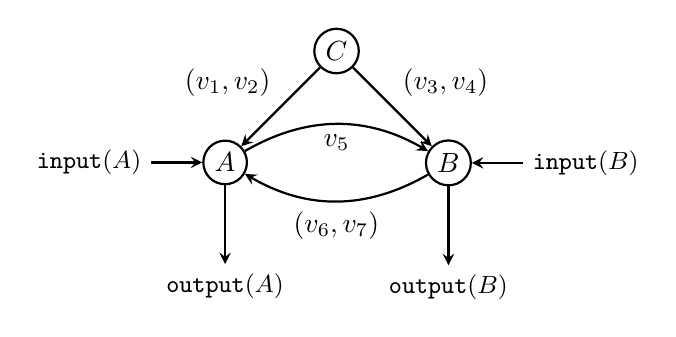
\begin{tikzpicture}
  %\useasboundingbox (-1,-1) rectangle (11,11); 
  \tikzset{DataStyle/.style = {draw=black, thick, shape=circle, inner sep=2pt, text=black}}
  \tikzset{OpStyle/.style = {draw=black, thick, shape=rectangle, inner sep=3pt, text=black}}
  \tikzset{EdgeStyle/.style   = {thick, ->, >=stealth, shorten <=0pt, shorten >=0pt}}
  \tikzset{PortEdgeStyle/.style   = {thick, ->, >=stealth, shorten <=0pt, shorten >=0pt}}


  \node(1)[DataStyle]{$C$};
  \node(2)[DataStyle, below left=of 1]{$A$};
  \node(3)[DataStyle, below right=of 1]{$B$};
  \node(4)[left=of 2, xshift=10pt]{{\small $\mathtt{input}(A)$}};
  \node(5)[right=of 3, xshift=-10pt]{{\small$\mathtt{input}(B)$}};
  \node(6)[below=of 2]{{\small $\mathtt{output}(A)$}};
  \node(7)[below=of 3]{{\small $\mathtt{output}(B)$}};
  
     \draw[EdgeStyle](1) to node[above left]{$(v_1, v_2)$} (2);
     \draw[EdgeStyle](1) to node[above right]{$(v_3, v_4)$} (3);
     \draw[EdgeStyle, bend left](2) to node[below]{$v_5$} (3);
     \draw[EdgeStyle, bend left](3) to node[below]{$(v_6, v_7)$} (2);
      \draw[EdgeStyle](4) to node{} (2);
      \draw[EdgeStyle](5) to node{} (3);
      \draw[EdgeStyle](2) to node{} (6);
      \draw[EdgeStyle](3) to node{} (7);



 \end{tikzpicture}
\label{fig:example-topology}
\caption{High-level synthesis sketch for secure multiplication}
\end{figure}

Next, let us fix a communication schedule between the parties.
%This will define the family of protocols we are interested 
%in, as shown in Figure~\ref{fig:example-topology}.
The structure of the protocol, as shown in Figure~\ref{fig:example-topology},
is as follows:\\
(1) $C$ computes some values $(v_1, \ldots, v_4)$ first ($5$ lines), \\
(2) $C$ sends $(v_1, v_2)$ to $A$ and  $(v_3, v_4)$ to $B$,\\
(3) $A$ computes $v_5$ ($1$ line) and sends it to $B$,\\
(4) $B$ computes some values ($3$ lines), 
sends a pair ($v_6$, $v_7$) to $A$ and picks one value as its output, \\
(5) $A$ computes its output ($2$ lines).\\
It is reasonable to assume that the user has a sketch such as above,
and we assume as such in this paper.
Nevertheless, even if such a structure is not available, one could either
pick a general-enough structure, or
iterate over such structures, to discover the desired protocol.
Hence, intuitively, our synthesis problem consists on
finding straight-line programs
$P_C, P_{A,1}, P_{B,1}, P_{A,2}, P_{B,2}$ such that
\begin{eqnarray*}
  (v_1, \ldots, v_4) &=& P_c(),
\\
v_5 &=& P_{A,1}(v_1, v_2, \mathtt{input}(A)),
\\
(v_6, v_7) &=& P_{B,1}(v_3, v_4, \mathtt{input}(B)),
\\
\mathtt{output}(A) &=& P_{A,2}(v_1, v_2, v_6, v_7, \mathtt{input}(A)),
\\
\mathtt{output}(B) &=& P_{B,2}(v_1, v_2, v_5, \mathtt{input}(B)),
\end{eqnarray*}
and $\mathtt{output}(B)$ and $\mathtt{output}(A)$
satisfy our correcteness requirement and the overall
protocol satisfies our security requirement.
%
%Here, when we say party $A$ computes some values
%with program $P_{A,1}$, we mean that party $A$ performs a 
%sequential composition of the components available to it; that is,
%$P_{A,1}$ is a straight-line program.
The set of components available to a party can vary, and this knowledge
can be specified in the input to the synthesis tool.  
We also assume we are given an upper
bound on the length of the straight-line programs
used by each party (shown in brackets above).   


The complete sketch is shown in Figure~\ref{fig:ex0}.
So far, the problem formulation
is similar to the component-based synthesis problem~\cite{bitvector}.
%
%Once we have the library of ten components, and the structure of the protocol
%above, we have what can be called a ``sketch'' of the protocol.  
%Now, we need
%to specify the requirements -- the functional correctness requirement
%$$\mathtt{output}(A) + \mathtt{output}(B) = \mathtt{input}(A)*\mathtt{input}(B),$$
%and the security requirement.

Let us first focus on the correctness requirement. If we give each of the $10$
components its natural interpretation (that is, all variables are 
integer valued, $\mathtt{plus}$ is arithmetic addition, and so on), 
then the correctness requirement is simply the arithmetic equality
$$\mathtt{output}(A) + \mathtt{output}(B) = \mathtt{input}(A)*\mathtt{input}(B).$$
Now, synthesis can be performed as in~\cite{bitvector} -- the synthesis problem
is reduced to an $\exists\forall$ formula over a suitable theory,
where $\exists$ quantifier searches over the space of possible programs,
and the $\forall$ quantifier checks correctness over the space of all possible
inputs. Note that, intuitively, this corresponds to 
generating candidate programs, and checking a {\em validity} property on
each of them. If the validity check passes, then the candidate is actually a solution.
Also, note that how to encode our security requirement in this formulation is not obvious.

%However, this approach does not work here because
%of two issues: first, 
%we have not captured the security requirement, and second,
%we have to solve an $\exists\forall$ problem over 
%the (undecidable) theory of nonlinear integer arithmetic.
Our new technique, bounded program synthesis, 
allows us to (a) turn the validity check above into a satisfiability
check over an alternative theory, resulting in a more efficient synthesis algorithm,
and (b) provide a natural way of specifying a nonfunctional security 
requirement. The key idea behind bounded program synthesis is
giving components a second, called {\em{dual}},
interpretation (as opposed to giving it the natural, or {\em{primal}}, interpretation).

\newcommand{\ttrule}[4]{{{#1}}: & \begin{array}{c}{#2}\\ \hline {#3}\end{array} &  {{#4}}}
\newcommand{\hoare}[3]{{\{{#1}\}\; {#2}\; \{{#3}\}}}

\begin{figure*}
    \begin{eqnarray*}
      \ttrule{\genx}{}{\hoare{\theta}{v := \genx}{\theta \circ \{v \mapsto pol2vec(``x'')\}}}{ v_x = 1 \;\wedge\; \bigwedge_{i\neq x} v_i = 0}
        \\
        \ttrule{\geny}{}{\hoare{\theta}{v := \geny}{\theta \circ \{v \mapsto pol2vec(``y'')\}}}{ v_y = 1\;\wedge\; \bigwedge_{i\neq y} v_i = 0}
        \\
        \ttrule{\plus}{[\theta(y)\neq y, \theta(z)\neq z]}%
        {\hoare{\theta}{x := \plus(y,z)}{\theta \circ \{x \mapsto \theta(y) + \theta(z)\}}}{ \bigwedge_{i\in I} x_i = y_i + z_i}
        \\
        \ttrule{\timess}%
        {[\theta(y)*\theta(z) \mbox{ is quadratic}]}%
        {\hoare{\theta}{x := \timess(y,z)}{\theta \circ \{x \mapsto \theta(y)*\theta(z)\}}}{ \bigwedge_{i,j\in L}x_{ij} = y_iz_j+y_jz_i \;\wedge\;\bigwedge_{i\in NL} y_i=z_i=0 }%
        \\
        \ttrule{\mathtt{compose}}%
        {\hoare{\theta_0}{P_1}{\theta_1} \qquad \hoare{\theta_1}{P_2}{\theta_2}}%
        {\hoare{\theta_0}{P_1;P_2}{\theta_2}}{}%
        \\
        \ttrule{\mathtt{check}}%
        {\hoare{\mathtt{id}}{P}{\theta} \qquad \theta(v)+\theta(w)=\theta(a)\theta(b)}%
        {\hoare{\mathtt{id}}{P}{\mathtt{assert(v+w=a*b)}}}%
        {v_{ab}+w_{ab}=1\;\wedge\; \bigwedge_{i\neq ab} v_i+w_i=0}%
      \end{eqnarray*}
      \caption{Proof rules and generated constraints for the secure multiplication example: The first two columns show named proof rules for proving an example assertion for a program in the class of programs considered in Section~\ref{sec:ex}.  Essentially, the rules perform symbolic execution of the program.  The third column shows (some of the) constraints that are generated on the dual variables. Some of the restrictions on the proof rules that are considered for performing bounded proof search are shown inside square brackets; for e.g., we use $\timess$ only on linear arguments because we want all generated symbolic expressions to be at most quadratic. The constraints are over dual variables: $v_i$ denotes the value of the coefficient of the $i$-th monomial in the symbolic value of $v$. The index $i$ ranges over $I=L\cup NL$, where $L = \{x,y,r,u,a,b\}$ and $NL$ consists of all quadratic monomials over $L$.}
  \label{fig:rules0}
\end{figure*}

As a first step in defining the dual semantics for this problem,
consider an abstract domain that consists of symbolic polynomial expressions
of degree at most $2$ over the six variables: the two inputs $a,b$ and the
four random numbers $x,y,r,u$.
$${\cal A} = \{p(a, b, x, y, r, u)~|~p\mbox{ is quadratic}\}$$
where polynomials in ${\cal A}$ are represented as lists of reduced monomials.

Let us say we wish our program (that is yet to be discovered)
to have a proof in this abstract domain.  
We can design proof rules that essentially perform
symbolic execution to check an assertion.
To do so, we assign an abstract value $\theta(v)$
to every line of the form $v:=op(\_)$
of our target program, where 
$op\in \mathtt{plus}, \mathtt{minus}, \mathtt{times}$
$\genx$,
$\geny$,
$\genr$,
$\gend$,
using a set of proof rules (see Figure~\ref{fig:rules0}).

We can use these proof rules to prove an assertion $v+w=a*b$ 
at the end of program $P$ as follows:
start with an identity substitution ($\mathtt{id}$), and update
it by symbolically executing the code. For example, 
in rule {\genx}, after execution
of $v := \genx$, we get a new substitution that maps $v$ to the symbolic
polynomial $x$. Similarly, 
rule {\plus},  handles program lines of the form 
$v := \plus(x, y)$ setting $\theta(v)$ to the polynomial $(\theta(x) + \theta(y))\in {\cal A}$.
Once we have the substitution $\theta$ resulting
after symbolically executing the whole program, we can check if 
$\theta(v)+\theta(w)$ and $\theta(a)*\theta(b)$ 
are identical expressions, i.e. correspond to the same element of the abstract domain ${\cal A}$.
The proof rule for $\timess$ in Figure~\ref{fig:rules0} has a condition
that allows multiplication to be used only on linear polynomials (so that
the result is atmost quadratic).
Note that, what we have done using this proof system to
check correctness is to turn our validity property over 
integers into an evaluation over ${\cal A}$.

Rather than searching for the correct program, let us say we want to
search for the proof in the proof system shown in Figure~\ref{fig:rules0}.  
Note that the
elements in the chosen abstract domain are parameterized
by $27$ parameters -- namely, the coefficients of all degree $1$ and degree $2$
monomials over the six variables ($C(6,1) + C(6,2) + C(6,1) = 6 + 15 + 6 = 27$).
Finding the proof is the same as finding the $27$ parameters for each program
line.
Let $L = \{x,y,r,u,a,b\}$ and $NL = \{ij \mid i\neq j, i\in L, j\in L\}\cup \{ii \mid i\in L\}$.
If $v$ is a program variable, then it is associated with
$27$ dual  variables, namely, $v_i$, where index $i$ ranges over the set
$I = L\cup NL$ of all indices. If variable $v$ gets a symbolic value
$p$, denoted  and $p$ is quadratic, then
the dual variables $v_i$'s get the value of the coefficient of the
monomial $i$ in $p$, which given the rules in Figure~\ref{fig:rules0},
will be a value in $\{-1, 0, 1\}$  
Now, let us say we could prove our functional requirement using quadratic
symbolic values.  Then, there exists a value of the dual variables that
witnesses this proof.  The converse is even more important: if
we find a value of the dual variables (a proof that relies on only
quadratic polynomials), then we would establish our functional requirement.

A sound proof rule application (on the abstract values) 
induces certain constraints on the dual variables.
Each proof rule corresponds to a component, so 
each component has to be associated with a suitable
constraint.  This constraint can be viewed as giving
``dual meaning'', a so-called {\em{dual interpretation}},
to the component.  This constraint essentially
says what combinations of these $27$
parameters for its inputs and outputs are consistent with the 
proof rule (that abstracts the primal semantics).
For example, the Column~$3$ in Figure~\ref{fig:rules0} shows
such constraints for each component.

Once we have these constraints, we just need to
search for the value of these $27$ parameters for the 
variables computed in the 
$11$ computation lines and the $7$ $\mathtt{identity}$ lines (used to model
the ``picking and sending'' operation) that are consistent with the
dual interpretation.
%and such that the required correctness formula
% is also provable in the abstract domain.  
Note that the correctness 
requirement was an equality of polynomial expressions, and in our
abstract domain, this maps to equality of coefficients 
(see right column on last row in Figure~\ref{fig:rules0}).
Thus, ignoring the security requirement, 
the synthesis problem is reduced to finding
$27*(11+7)$ values that satisfy some big constraint generated 
using the dual interpretation.  This is an $\exists\exists$ problem:
we are finding a program (first $\exists$) and a proof of its correctness over
the chosen abstract domain (second $\exists$).
Duality has enabled us to replace the $\forall$ check by an 
$\exists$ check.

We still have not solved our original problem because we still need to
include the security requirement.  The formal security requirement
{\em{check: (that is based on showing the existence of a simulator that can generate
values close to the synthesized protocol using an ideal secure protocol
as an oracle)}} is difficult to capture precisely. 
We take a very practical approach here:  we replace the security requirement
by another easily checkable requirement that is sufficient (but not necessary)
for security.  The new check can itself be described by 
proof rules, and we can again search for a bounded-size proof
to establish security.
The sufficiency of the proof rules may itself be proved as a 
meta-theorem by hand.  In some cases, we may not get a simple 
enough set of proof rules that is
provably sufficient. In these cases, we use an approximate proof
rules, and in 
such cases, our synthesizer will generate protocols that are correct, and most
likely secure, but security needs to be re-evaluated in a post processing step.

\begin{figure*}
  \begin{tabular}{|l|l|}
    \hline
    security requirement (a) & 
    $\mathtt{isrand(val@(CA,1))} \wedge
     \mathtt{isrand(val@(CA,2))} \wedge
     \mathtt{isrand(val@(CB,1))} \wedge
     \mathtt{isrand(val@(CB,2))} \wedge$
     \\ &
     $\mathtt{isrand(val@(AB,1))} \wedge
     \mathtt{isrand(val@(BA,1))} \wedge
     \mathtt{isrand(val@(BA,2))}
    $
    \\
    security requirement (b) &
    $\bigwedge_{S_1\subseteq S}  \bigoplus_{v\in S_1} \mathtt{rseeds}(v) \neq \langle 0,0,0,0\rangle$ {\mbox{ where }} 
    $S = \{\mathtt{ val@(CA,1), val@(CA,2), val@(BA,1), val@(BA,2)} \}$
    \\ &
    $\bigwedge_{S_1\subseteq S}  \bigoplus_{v\in S_1} \mathtt{rseeds}(v) \neq \langle 0,0,0,0\rangle$ {\mbox{ where }} 
    $S = \{\mathtt{ val@(CB,1), val@(CB,2), val@(AB,1)} \}$
    \\ \hline
\end{tabular}
\caption{Security requirements captured as constraints on the dual
values computed at the various program points. The function
$\mathtt{isrand}$ checks if the value (computed at the given program
point) is ``random'' and 
$\mathtt{rseeds}$ returns the randomly-picked numbers that are used
to compute the value (computed at that program point, in 1-hot encoding).}
\label{fig:secure0}
\end{figure*}

For our example, we capture the security requirement by checking that 
(a) every value that is exchanged between the parties are ``random'',
and
(b) none of the parties can possibly eliminate all random seeds from
any value it gets from others using all the other values it gets from others.
We do not need a new proof system here because we can piggyback on the
dual interpretation used earlier.
For (a), we call a value (computed at a line) ``random'' 
if the symbolic polynomial expression representing the value computed
at that line contains one of the four random seeds ($x$, $y$, $r$, or $u$).
For example, $ab$ is not random, but $ax$ is random.
Let $\mathtt{rseeds}(v)$ be a bitvector of length $4$ that denotes if
$x$, $y$, $r$, or $u$ is present in $v$.
If $\mathtt{rseeds}(v) = \langle b_1,b_2,b_3,b_4\rangle$,
then define
$\mathtt{isrand}(p)$  to be the Boolean value
$b_1\vee b_2\vee b_3\vee b_4$.
The constraints that encode the
security requirement are shown in Figure~\ref{fig:secure0}. 

The logic to capture requirement (b)  is also shown in
Figure~\ref{fig:secure0}. It is fairly simple too. 
For example, if Alice obtains a set $S = \{v_1, v_2, \ldots\}$ of values
from Bob and Carol, then we check if, for some subset $S_1\subset S$ of $S$,
it is the case that
\begin{eqnarray*}
  \bigoplus_{v \in S_1}  \mathtt{rseeds}(v) & = & \langle 0,0,0,0\rangle
\end{eqnarray*}
where $\oplus$ denotes bitvector exclusive-or (xor).
If the above is true for some $S_1$, then we declare that Alice can
possibly learn something (that it should not learn) from the values it receives,
and hence, such protocols are considered to fail the security requirement.
For example,
if Alice receives values $bx$ and $b-bx$ (from Bob), then
\begin{eqnarray*}
  &&\mathtt{rseeds}(bx) = \langle 1,0,0,0\rangle,
\;\; 
\mathtt{rseeds}(b-bx) = \langle 1,0,0,0\rangle,
\\ &&
\mathtt{rseeds}(bx) \oplus \mathtt{rseeds}(b-bx) = \langle 0,0,0,0\rangle,
\end{eqnarray*}
Hence, this indicates Alice can possibly learn something new from the messages.
In this case, Alice can indeed learn $b$ (since $b = bx + (b-bx)$).
Clearly, this is a conservative check. For example,
if $v_1 = bx$ and $v_2 = bx$, then 
$$
\mathtt{rseeds}(bx) \oplus \mathtt{rseeds}(bx) = \langle 0,0,0,0\rangle.
$$
However, in this case, Alice can not learn $b$ from $bx$ (unless 
it also knows the random number $x$), while our check concludes otherwise.


\begin{figure}[ht]
  \begin{tt}
    \begin{tabular}{|ll|}
      \hline
      block C: & $v_1 := \genx; v_2 := \geny; v_3 := \genr;$
      \\
                 & $v_4 := \timess(v_1,v_2); v_5 := \minus(v_3,v_4)$
      \\
      block CA: & $v_5 := \identity(v_1); v_6 := \identity(v_3)$
      \\
      block A1: & $v_7 := \inputa$
      \\
      block $\mathtt{A2}$: & $v_8 := \minus(v_7, v_5)$
      \\
      block $\mathtt{AB}$: & $v_9 := \identity(v_8)$
       \\ 
       block $\mathtt{CB}$: & $v_{10} := \identity(v_5); v_{11} := \identity(v_2)$
       \\ 
       block $\mathtt{B1}$: & $v_{12} := \inputb$
       \\
       block $\mathtt{B2}$: & $v_{13} := \plus(v_{11}, v_{12}); v_{14} := \timess(v_9,v_{12});$ 
       \\ &
       $v_{15} := \plus(v_{14}, v_{10})$ 
       \\ 
       block $\mathtt{BA}$: & $v_{16} := \identity(v_{13})$ 
       \\ 
       block $\mathtt{A3}$: & $v_{17} := \timess(v_{16}, v_5); 
       v_{18} := \minus(v_{17}, v_6)$
       \\ 
       block $\mathtt{B3}$: & $v_{18} := \identity(v_{15})$
       \\ \hline
    \end{tabular}
  \end{tt}
  \caption{The synthesized secure multiplication protocol. This is the 
    same program whose English description is provided in the text. It is 
  discovered by our synthesis tool using the inputs shown in 
Figure~\ref{fig:ex0}, Figure~\ref{fig:rules0}, and Figure~\ref{fig:secure0}.}
\end{figure}

With this encoding of the security requirement, our sketch is complete,
we run our synthesis tool, and it returns the following protocol:
\begin{enumerate}
  \item
    $C$ generates random numbers $x,y,r$, and computes $xy$ and $r-xy$
  \item
    $C$ sends $(x,r)$ to $A$ and $(r-xy,y)$ to $B$
  \item
    $A$ computes $a-x$ and sends it to $B$
  \item
    $B$ computes its share $(a-x)b + (r-xy)$ and sends $y+b$ to $A$
  \item
    $A$ computes its share $(y+b)x-r$
\end{enumerate}
We were not aware of this protocol before it was synthesized by our tool.
Note that the protocol did not use the fourth random number ($u$), whereas
we were expecting the synthesized protocol to need it.


\section{A Simple Programming Language Abstraction}
\label{sec:language}

We formalize a simple programming model in this section that
admits both primal and dual variables.
Our presentation abstracts away the concrete syntax for program statements.  
Our goal here is to differentiate between the primal and dual components of 
a program at a semantic level.
% interpretations 
% we will define both {\em{primal}} and {\em{dual}} semantics that can be
% assigned to such programs.

Let $\Vp$ and $\Vd$ denote two finite sets.
We call $\Vp$ primal program variables and 
$\Vd$ dual program variables.
Let $\domp$ and $\domd$ denote two domains of values.
The set $\psp$ of all primal states is
just the set of all mappings from primal 
variables $\Vp$ to the domain $\domp$.
Similarly, the set $\psd$ of all dual states is
the set of all mappings from dual 
variables $\Vd$ to the domain $\domd$.
\begin{eqnarray*}
  % \mathit{Program\ \ states}
  \psp \; := \;
  \{ \sigma: \Vp \rightarrow \domp \}
& \quad &
  \psd \; := \;
  \{ \ds: \Vd \rightarrow \domd \}
\end{eqnarray*}
We note that
a program state is just a substitution and hence
we chose $\sigma$ or $\ds$ to denote a state.

Rather than fixing a syntax for program statements,
we just define program statements semantically.
Primal program statements, denoted by $\Stmtp$,
are just mappings (transformers) from sets of primal states to 
sets of primal states.
On the other hand, dual program statements, denoted by $\Stmtd$,
are just subsets of (constraints on) the set of all dual program states.
\begin{eqnarray*}
 \Stmtp \;\; := \;\; \{ T: 2^\psp \rightarrow 2^\psp \}
& \qquad\qquad &
 \Stmtd \;\; := \;\; 2^{\psd}
\end{eqnarray*}

If $T\in\Stmtp$ is a primal program statement,
and $S\subset \psp$ is a subset of program states,
then $T(S)$ is a set of program states, which
intuitively represents the states reached from $S$
after ``executing'' the program statement $T$.
A dual program statement $\phi\in\Stmtd$ is simply a constraint
on dual variables (constraining their admissible values).

A {\em{program}}  $P$ is a graph
$(V, E, l_p, l_d, v_s, v_e)$, where
% \\
% \begin{itemize}\itemsep=0em
% \item
(a) $V$ is a set of nodes,
% \\
% \item
(b) $E \subset V^2$ is a set of directed edges,
% \item
% \\
(c) $l_p: E \rightarrow \Stmtp$ is a function that labels all edges in $E$
by primal program statements in $\Stmtp$, 
% \\
(d) $l_d: E \rightarrow \Stmtd$ is a function that labels all edges in $E$
by dual program statements in $\Stmtd$, and
% \item
% \\
(e) $v_s, v_e \in V$ are designated start and end nodes.
% \end{itemize}

% We deliberately do {\em{not}} define the set $\Stmt$ of statements.
% For our purposes, $\Stmt$ is just a set.
% Since our goal is to highlight how a dual semantics differs from
% a primal semantics, it is beneficial to abstract the details of
% a program statement in this way.
% All we need to know about $\Stmt$ is that
% it manipulates values of a fixed set
% $\V$ of program variables.

\ignore{

Before we can define the set $\Stmt$ of statements, we first
need to define the
expression language.
Let us assume we
have a signature
$\Sig$ consisting of constant symbols,
function symbols, and predicate symbols,
with their arities.
Constant and function symbols are used to create
terms in the usual way, whereas
predicate symbols are applied on terms to create
Boolean-valued expressions.
We use $x,y$ to denote program variables, and we use
$f(\vec{x})$ to denote the expression obtained by
applying $f\in\Sig$ to a sequence of program variables
whose length equals the arity of the function or predicate
symbol $f$. We use
$\Tau(\Sig,\V)$ to denote all terms constructed
using the signature $\Sig$ and free variables $\V$.

Given a signature $\Sig$ and a set $\V$ of program variables,
the set $\Stmt$ of program statements consists of two kinds of
statements:
\begin{itemize}\itemsep=0em
\item {\em{assignment}} statements of the form
    $x := f(\vec{x})$, where $x \in \V$,
    $f\in\Sig$ is a function symbol of arity, say, $n$, and
    $\vec{x}$ is a sequence of program variables whose length is equal to $n$.
    Note that, in particular, $f$ can be a constant with arity $n = 0$.
\item {\em{assume}} statements of the form
    $\assume(p(\vec{x}))$, where $p\in\Sig$ is a predicate symbol of arity, say, $n$,
    and $\vec{x}$ is a sequence of program variables whose length is equal to $n$.
\end{itemize}

\endignore}

\begin{remark}
To provide readers concrete intuition, the set $\Stmtp$ can be viewed
as the meanings of standard {\em{assignment}} statements and
%ADRIA: While assignment statements are crucial for some definitions,
% assume statements are not mentioned later
{\em{assume}} statements.
% defined over the set $\V$ of program variables
%(using some set of constants, function symbols, and predicate symbols).
A node with two or more outgoing edges denotes a {\em{non-deterministic}}
branch, and can be used to model a conditional statement by having
\assume\ statements label the outgoing edges.
A node with two or more incoming edges is a control flow merge point.
A loop is manifested as a ``backward'' edge in the graph that creates
a directed cycle.
\end{remark}
%The syntax of our language is presented in Figure~\ref{fig:language}.
%A program is just a (sequentially composed) sequence of statements.
%followed by an assertion.
%A statement is either an assignment statement, conditional
%statement or a loop.
%An assignment statement is of the form
%$x := f(\vec{x})$, where $f\in\Sig$ is a function
%symbol with arity, say $n$, and $\vec{x}$ is a sequence of $n$
%program variables. In particular, $f$ can be a constant with
%arity $n = 0$.
%A conditional statement is of the form
%${\iteif} \; (c) \;{\itethen}\; {\tt{Prgm}} \;{\iteelse} \; {\tt{Prgm}} \; {\itefi}$,
%where ${\tt{Prgm}}$ is just a sequentially composed
%sequence of statements, and
%the condition $c$ is simply a predicate $p\in\Sig$
%with arity, say $n$, applied to $n$ program variables.
%A loop is of the form
%${\textit{while}} \; (c) \;\{ \; {\tt{Prgm}} \; \}$,
%where $c$ is a condition as before.

\ignore{

\subsection{Primal Semantics of Expressions}
Before we define what constitutes a primal semantics of a program,
we need
to fix the meaning of expressions.
This is done by using a {\em{structure}}
$(\dom, \int)$
where the domain $\dom$ is a nonempty set, and the interpretation
$\int$ maps
\\
(a) every constant $c\in\Sig$ to an element $c^\int\in\dom$,
\\
(b)
every function symbol $f\in\Sig$ with arity $n$ to a
concrete function $f^\int: \dom^n\mapsto\dom$, and
\\
(c)
every predicate symbol $p\in\Sig$ with arity $n$ to a
subset of $\dom^n$.

For example, $\dom$ could be the set of integers, or machine integers,
or length $n$ bitvectors.
If $\dom$ consists of bitvectors, $\int$ could map a symbol
$\oplus$ in $\Sig$ to the bitwise xor operator.

The mapping $\int$ is extended to a mapping over all ground terms
$\Tau(\Sig,\emptyset)$ in the usual way:
specifically,
\begin{itemize}
  \item if $f$ is a arity $n$ function symbol, then
$f(t_1,\ldots,t_n)^\int$ is defined as $f^\int(t_1^\int,\ldots,t_n^\int)$
recursively; and
\item
if $p$ is a arity $n$ predicate symbol, then
$p(t_1,\ldots,t_n)^\int$ is defined as the Boolean value indicating
if the $n$-tuple
$(t_1^\int,\ldots,t_n^\int)$ is in $p^\int$.
\end{itemize}
Intuitively, the primal meaning of any term in $\Tau(\Sig,\emptyset)$
is just its evaluation (to a value in $\dom$ or a Boolean value)
in the underlying structure $(\dom,\int)$.

We will treat applications of function (or predicate)
$f\in\Sig$ as ``library'' calls. For simplicity, we assume
these calls always return with the (semantically) correct
values, and erroneous behaviors, which cause runtime exceptions or
nontermination, do not occur.

\endignore}

\ignore{
\subsection{Primal Program Semantics}

A program is simply a transformer from a set of program states
to a set of program states. We define this transformer
more formally in this section. The purpose behind presenting
the primal semantics, which is fairly standard, is that it will
be used later to contrast it with the dual semantics.

Assuming $\V$ is the set of all program variables,
a (primal) {\em{program state}} is simply a mapping from the
set $\V$ of program variables to values in some domain $\dom$ of values.
We use the symbol $\sigma$, possibly with subscripts or superscripts,
to denote a program state.
The set of all {\underline{p}}rimal
{\underline{p}}rogram
{\underline{s}}tates is denoted by $\pps$.
\begin{eqnarray}
  % \mathit{Program\ \ states}
  \pps & := &
  \{ \sigma: \V \rightarrow \dom \mid \mathtt{True} \}
  \label{eqn:primalStates}
\end{eqnarray}
We note that
a program state $\sigma$ is just a substitution.

%Note that $\int$ defines the meaning of all ground
%expressions in $\Tau(\Sig,\emptyset)$.
%A program state gives meaning to variables in $\V$, and
%thus, a program state, together with the structure
%$(\dom,\int)$, provides meaning to any expression
%in $\Tau(\Sig,\V)$.

Given a program $P$, how do we define the transformer from
program states to program states that captures its meaning?
It is evident that the exact transformer will depend on the meaning
assigned to individual statements that constitute $P$. Hence, let
us assume we
are given a function $\sem$ that assigns meanings to individual
program statements.
% Let $\pps$ denote the set of all possible mappings from
% Let $s\in\Stmt$ denote a single program statement.
\begin{eqnarray}
 \sem & : & \Stmt \rightarrow 2^\pps \rightarrow 2^\pps
 \label{eqn:primalOne}
\end{eqnarray}
If $s\in\Stmt$ is a single program statement,
and $S\subset \pps$ is a subset of program states,
then $\sem(s)(S)$ is a set of program states, which
intuitively represents the states reached from $S$
after ``executing'' the program statement $s$.

\endignore}

\subsection{Primal and Dual Program Semantics}

Given a program $P$ as defined above, we can now define
its semantics in two parts: the primal $\semp$ and the dual $\semd$ semantics. 
% We now lift the function $\sem$ that is defined for
% singleton program statements $s$ to a sequence
% of program statements.
Let $\pi := \langle v_0, e_1, v_1, e_2, \ldots, e_{k}, v_k \rangle$ be a path 
containing vertices $v_i$'s and edges $e_i = (v_{i-1},v_i)$ in the program $P$.
%  that is,
% $$
 % l(\pi) = \langle l((v_0,v_1)), l((v_1,v_2)), \ldots, l((v_{k-1},v_k))\rangle
% Let $T_1;\ldots;T_m$ be a sequence of primal program statements.
In the primal case, the meaning of a path is 
the composition of the transformers in that path, whereas
in the dual case, it is  the conjunction (intersection).
\begin{eqnarray}
  \semp(\pi)(Sp) & = &  l_p(e_k)(l_p(e_{k-1})( \cdots l_p(e_1)(Sp)\cdots)) \\
  \semd(\pi)(Sd) & = &  Sd \cap  \bigcap_{i=1}^{k} l_d(e_i)
\end{eqnarray}
%
% Let $P$ be a given program.

The primal meaning of $P = (V,E,l_p,l_d,v_s,v_e)$ is defined by
taking the union over all paths
from the start node $v_s$ to the end node $v_e$ in $P$, and the
dual meaning is obtained by taking the conjunction.
\begin{eqnarray}
 \semp(P)(Sp) & = &
  \bigcup_{\pi\in\paths(v_s,v_e)}
   \semp( \pi )(Sp)
\\
 \semd(P)(Sd) & = &
  \bigcap_{\pi\in\paths(v_s,v_e)}
   \semd( \pi )(Sd)
 %\label{eqn:primalProgram}
\end{eqnarray}
where $\paths(v_s,v_e)$ denotes the set of all paths from $v_s$ to $v_e$ in $P$.

%Note that $\sem(P)(S)$ might be infinite.
% ADRIA: This comment should make the reader think about least fixed points

\ignore{
\subsection{Dual Program Semantics}
\label{sec:dual}

In this section, we present a slightly different way of
assigning meanings to programs, which we refer to as
dual semantics of programs.

Recall the four main steps involved in building a primal
semantics; namely,
%\\
(a) defining the set of program states
(Equation~\ref{eqn:primalStates}),
%\\
(b)
assuming some given meaning for individual statements
(Equation~\ref{eqn:primalOne}),
%\\
(c) lifting the meaning for one statement to a sequence of statements
(Equation~\ref{eqn:primalPath}),
and
%\\
(d) defining the primal meaning for a program from that of
individual paths
(Equation~\ref{eqn:primalProgram}).
We perform four similar steps for the dual semantics to highlight
the differences between the primal and the dual case.



\subsection{Dual Program States}

A {\em{dual program state}} is a mapping from the
set $\Vt$ of dual program variables to values in some domain $\domt$ of dual values.
As we did in the case of the primal semantics, we let the set $\domt$
be some abstract set.

How is the set $\Vt$ of dual program variables related to the program $P$?
Essentially, every program location gives rise to a dual variable.
We formalize this correspondence by a mapping $\vmap$ from the set $E$ of
edges in the program $P$ to the set $\Vt$:
\begin{eqnarray*}
  \vmap:   E \rightarrow \Vt
\end{eqnarray*}
It is often the case that this map is a bijection, but one could,
as part of the dual semantics specification,
have {\em{any}} surjective function here.

The set of all dual program states is denoted by $\dps$.
\begin{eqnarray}
  % \mathit{Program\ \ states}
  \dps & := &
  \{ \ds: \Vt \rightarrow \domt \mid \mathtt{True} \}
  \label{eqn:dualStates}
\end{eqnarray}

Intuitively, in one possible use,
the dual variable corresponding to an assignment statement
can be thought of as storing the ``type'' of the left-hand side variable
in the assignment. The dual variable corresponding to an \assume\ statement
can be thought of as storing some ``information'' about the condition that
could influence the ``type'' of later assignments.

%Adria: I do not understand the previous sentence

\begin{remark}
  The dual variables essentially correspond to the program locations.
  We could have used $E$ as $\Vt$, but there are two reasons for
  introducing the set $\Vt$: first, it avoids confusion that could
  be generated by having edges in $E$ treated as dual program variables, and
  second, $\vmap$ additionally gives the flexibility of assigning the
  same dual variable to two or more different program locations.
\end{remark}


% \subsection{Dual Semantics of a Single Path}

....HERE ....HERE ....still working...
In the case of the primal semantics, we had assumed that we are given
the meaning of each individual statement.
In the dual semantics, we assume we are given the meaning of
paths in the program.
% We now move to defining the (dual) meaning of a single statement.
%In the case of the dual semantics, however, the signature of
%this semantics function is quite different.
Let $u,v\in V$ be two nodes in the program $P$.
The dual semantics function, $\semt_\vmap$,
depends on the mapping function $\vmap$ and maps
a path $\pi\in\paths(u,v)$ to a set of (dual) states.
% {\em{depending}}
% on the statements in the path in $P$ that led to $s$.
\begin{eqnarray}
 \semt_\vmap & : & V^* \rightarrow 2^\dps
 \label{eqn:dualOne}
\end{eqnarray}
Here, $V^*$ denotes the set of all finite sequences of nodes $V$ in $P$.
Of course, the intention is that these sequences correspond to paths in $P$.

Assuming all variables used in the program fragment $\pi$ are also
defined in $\pi$, the constraint $\semt_\vmap(\pi)$ 
% defines a relationship between the different 
only constrains the dual variables on the path; that is, dual variables
in the set $\{\vmap(e) \mid e\mbox{ is an edge in the path } \pi\}$.
This is the reason why $\semt$ is subscripted by the function $\vmap$.
% In particular, $\semt(s,l(\pi))$ is defined when $\pi$ is a
% path from the initial node $v_s$ to an edge that is labelled with $s$.

\begin{remark}
  In the primal semantics, a program statement is the basic entity that is
  used to define the meaning of the whole program.
  In the dual semantics, a program path is such a basic entity.
  In the dual semantics, a path is not a transformer on dual program
  states. In contrast, it is just a {\em{constraint}} that defines a subset of
  dual states. % that {\em{depend}} on the path taken to
  % reach the statement.
\end{remark}

\begin{remark}
If the dual semantics captured in $\semt$
is generating ``well-typedness'' constraints for the
program, then the $\semt$ function needs to know
at which program point a certain variable was last defined,
and which $\assume$ conditions were tested before; and hence,
the basic entity for defining $\semt$ is a program path.
\end{remark}

\subsection{Dual Semantics of Multiple Paths ending in a Node}

In the primal case, % once we have the meaning of a single statement,
we used sequential composition to assign meanings to sequences of primal program statements.
In the dual case, % using the meaning of a path, we move on to defining
we used logical conjunction as the meaning of a sequence of dual program statements.
% the meaning of a collection
% of paths starting from the node $u$ and ending on the node $v$.
% individual statements are not
% transformers, but just constraints.
The meaning of a path
is just the conjunction of (the constraints generated by) each dual statement in the path.
% Thus, given a function
 % $\semt_\vmap : V^* \rightarrow 2^\dps$, we get a new function
 % $\semt_\vmap : V \rightarrow V \rightarrow 2^\dps$ as follows:

\begin{eqnarray}
  \semt_\vmap(u)(v) & = & \bigcap_{\pi\in\paths(u,v)} \semt_\vmap(\pi)
  %\lefteqn{\semt_\vmap(\langle s_1,\ldots,s_m\rangle)(\pi)} &   &
  %%\nonumber
  %\\ & = &
  %\bigcap_{i=1}^{m} \semt_\vmap(s_i)(\pi.s_1.\ldots.s_{i-1})
 \label{eqn:dualPath}
\end{eqnarray}

% Note that before taking the meaning of $s_i$, we append the path
% $s_1,\ldots,s_{i-1}$ to the base path $\pi$.

\begin{remark}
In the dual semantics, every program path emits a constraint.
Across multiple paths, we just take the conjunction of the constraints emitted
by each path. In contrast, in the primal semantics, we used a union
across multiple paths.
% Since the constraint has to be on the dual variables, we need
% to know the mapping from program points to dual variables.
% Hence, $\semt$ is subscripted by the function $\vmap$.
% Furthermore, the $\semt$ function may also need to know
% at which program point a certain variable was last defined,
% and which $\assume$ conditions were tested in the path.
% Hence, $\semt$ takes the path as an argument.
\end{remark}


\subsection{Dual Semantics of a Program}

Finally,
the meaning of a program $P = (V,E,l,v_s,v_e)$ in
a dual semantics is given by
taking the {\em{conjunction}} over all the meaning
assigned to pairs of {\em{essential}} vertices in $P$.
A vertex $v\in V$ is {\em{essential}} if it occurs on
all paths from $v_s$ to $v_e$.
Let $EV = \{v_0,\ldots,v_m\}\subset V$ denote the set of all essential vertices
in program $P$ ordered by the program line number, i.e.\ according 
to some topological ordering of $P$.
We can now define the function
$\semt_\vmap: \mathtt{Program} \rightarrow 2^\dps$ as follows:
\begin{eqnarray}
 \semt_\vmap(P) & = &
  \bigcap_{i=1}^m \semt_\vmap(v_{i-1})(v_i)
  %\!\!\!\!\!\!\!\!\!\!\bigcap_{\pi\in\paths(v_s,v_e)}
   %\!\!\!\!\!\!\!\!\!\!\!\!\semt_\vmap( l(\pi) )(\pi')
 \label{eqn:dualProgram}
\end{eqnarray}
%where $\paths(v_s,v_e)$ denotes the set of all paths from $v_s$ to $v_e$ in $P$.
% The dual meaning of a program $P$ is simply
 % $\semt_\vmap(P)(\epsilon)$, where $\epsilon$ is the empty path.
We can now match the signature of $\semt$ function with that of the
$\sem$ function (defining the primal semantics) by defining the dual
semantics of a program as a transformer on set of states as follows:
\begin{eqnarray}
 \semt_\vmap(P)(S) & = & S \cap \semt_\vmap(P)
\end{eqnarray}
Note that we use the same name $\semt_\vmap$, but with the new signature
$\semt_\vmap: \mathtt{Program} \rightarrow 2^{\dps} \rightarrow 2^\dps$.

\endignore}

Intuitively, the set $\semp(P)(Sp)$ is the set of primal program states reachable from some initial
state in $Sp$ by ``executing'' the (primal component of the) program $P$.
The primal semantics captures the standard meaning of programs.
%The set $\semd(P)(Sd)$ is the set of dual program states that are consistent with 
%each constraint generated in the program and the inital constraint $Sd$.
%
%
%Intuitively, in the dual interpretation, 
In the dual semantics, a program starts with a set of
possible {\em{admissible}} dual states $Sd$ (initial states) and eventually
finds a state (or a set of states) from $Sd$ that is {\em{consistent}} with
the program $P$.
% Subsequently, we do not explicitly show the subscript $\vmap$ in the
% $\semt_\vmap$ notation to make the dual semantic transformer
% function appear as the primal transformer $\sem$.

For a program that has both a primal and a dual component, we can now define its
combined semantics by defining its state space as the Cartesian product of the primal
and dual state spaces, and doing the same for the primal and dual semantics.


\section{Primal and Dual Assertion Checking}
\label{sec:assertionchecking}

We defined the primal and dual semantics of programs as
transformers on sets of, respectively, primal and dual states.
We now highlight the
key difference between a primal and a dual semantics,
which is in the, respectively, demonic and angelic,
interpretation assigned to nondeterminism.

If a set $S$ of (initial) states is transformed to a set
$S'$ (in either the primal or dual semantics), then we
say that $S'$ is reachable from $S$.
In the primal semantics, nondeterminism is {\em{demonic}}:
a post-condition holds (at the end of the program) if
{\em{every}} reachable state from an initial state
(in the primal semantics)
satisfies the post-condition.
In the dual semantics, nondeterminism is {\em{angelic}}:
a post-condition holds if
there exists
{\em{some}} reachable state (in the dual semantics)
that satisfies the post-condition.
Moreover, primal semantics are naturally computed using a
least fixpoint computation, whereas dual semantics are
computed using a greatest fixpoint computation.

This difference in the interpretation of nondeterminism
is reflected in the following formulation of the primal
and dual assertion checking problems.

\begin{definition}[Assertion checking problem]
  Given a program $P$, 
  % a primal semantic function for
  % individual program statements in $P$,
  a set of primal initial states $U$,
  and a primal assertion $x=c$,
  where $x$ is a primal program variable and
  $c\in\domp$ is a constant,
  the {\em{primal assertion checking problem}} seeks to determine if
  $\sigma(x)=c$ for \underline{all} program states $\sigma$
  in $\semp(P)(U)$.

  Given a program $P$,
  % a dual semantic function for individual program paths in $P$,
  a set of dual initial states $U$,
  and a dual assertion $x\approx c$,
  where $x$ is a dual program variable and
  $c\in\domd$ is a constant in the dual domain,
  the {\em{dual assertion checking problem}} seeks to determine if
  $\sigma(x)=c$ for \underline{some} program state $\sigma$
  in $\semd(P)(U)$.
\end{definition}

\begin{figure*}[tb]
  \begin{center}
  \begin{tabular}{||c||c|c|c||}
    \hline
    Program & Dual 1 & Dual 2 & Dual 3
    \\ \hline \hline
    $l_0:\; \mathtt{input}\; x; $ & $\neg l_0$ & $l_0=\float$ & $l_0 \geq 0$ \\
            $l_1:\; y := 0.0 ;$ & $\true$ %Adria: Shouldn't this be $l_1$
            & $\true$ %Adria: Shouldn't this be $l_1=\zero$
            & $l_1 \geq 0$ \\
            % $l_2:\; z := y*x ;$ & $l_2\Leftarrow l_0\wedge l_1$ & $\substack{l_2\neq\zero\Leftarrow (l_0\neq\zero\vee l_1\neq\zero)\wedge \\ l_2=\float\Leftarrow (l_0=\float\vee l_2=\float)}$ & $l_2\geq l_0+l_1+1$\\
            $l_2:\; z := y*x ;$ & $l_2\Rightarrow l_0\wedge l_1$ & ${l_2=\zero\Rightarrow (l_0=\zero\vee l_1=\zero)\wedge}$ & $l_2\geq l_0+l_1+1$\\
                                  & & $l_2=\int\Rightarrow (l_0\neq\float\wedge l_1\neq\float)$ & \\[0.4ex]
           $l_3:\; x := 1 + z;$ & $l_3\Rightarrow l_2$ & ${l_3\neq\zero \wedge (l_3=\int \Rightarrow l_2\neq\float)}$ & $l_3 \geq l_2$
    \\ \hline
  \end{tabular}
\end{center}
  \caption{{\small{Illustrating multiple dual components that can be associated to the same primal straight-line program.
    % Assertion $x=1$ holds at the end of the program in the primal semantics, whereas
    The assertion $l_3 \approx \true$ does {\em{not}} hold in the first dual program.
    Both the assertions $l_3\approx\int$ and $l_3\approx\float$ hold in the second dual program.
    Finally, the assertion $l_3 \approx 1$ holds in the third dual program.
  %assertion $x:\integers$ (and the assertion $x:\floats$) holds at the end of the program in the dual semantics.
  }}}\label{fig:ex1}
\end{figure*}

\subsection{A Simple Straight-Line Program Example}

Consider the simple four line program in
Figure~\ref{fig:ex1} (column 1) and let us refer to it as $P$.
If we take the natural interpretation of the arithmetic
symbols over the (primal) domain consisting of all numbers
($\domp$ = set of all numbers), then we naturally obtain the
meaning of $P$ as a transformer that
maps any initial state 
$(x,y,z)$ to a final state
$(x=1, y=0.0, z=0)$. 
% Hence, for every set of initial states $S$,
% $\semt(P)(S)$ is $\{\{(x,1), (y,0.0), (z,0)\}\}$.
%Adria: I added this sentence to have the example in exactly the
%same terms than the definitions above
In particular, under this natural (primal) semantics, the assertion
$x=1$ holds at the end of the program (because it holds for
{\em{all}} states reachable from {\em{any}} initial state).

%\begin{remark}
%We note that we introduced, as line $l_0$ in the example in Figure~\ref{fig:ex1},
%the statement $\mathtt{input}\; x$.
%%Adria: we could mention the input statement  in remark 1
%Apart from identifying that $x$ is an input here, it also serves the purpose of
%creating a dual variable (corresponding to line $l_0$) that can be used to
%carry constraints on the input values.
%\end{remark}

We now define three different dual components that can be combined
with this primal program.
In all the three cases, $l_0,l_1,l_2,l_3$ are the four dual program variables.
The first dual program is shown in Column titled ``Dual 1'' in 
Figure~\ref{fig:ex1}.
The dual domain, $\domd$, is $\{\true,\false\}$, and the four
program statements are associated with four different constraints
(on the dual variables).
Note that we have not yet defined what is a ``correct'' dual component
for a given primal program.  Informally, however, the
dual variables in the ``Dual 1'' program have a meaning:
if the dual variable $l_i$
is assigned $\true$, then the value computed on line $l_i$ in the primal
is definitely a ``constant'' value, whereas if it is $\false$,
then the value {\em{may or may not}} be a ``constant'' value.
The four constraints defining the dual semantics ``Dual 1'' 
propagate information pertaining
to whether a value (computed at line $l_i$ in the primal) is a
constant.
%Since this is a straight-line program and every node is essential, 
%the paths of interest
%%Adria: Changing this back 
%%are the four length $1$ paths in the program graph.
%are the ones from the initial node to every other node, 
%represented by lines $l_0, \ldots, l_3$.
%The first dual program, shown in Column titled ``Dual 1'',
%is designed to properly propagate the ``is-a-constant'' information.
For example, the constraint on the third line says that
if $l_2$ is $\true$ ($z$ is known to be a constant value), then
necessarily $l_0$ and $l_1$ should be $\true$ ($x$ and $y$ should be constant
values).
%Since all vertices in a straight-line program are essential, we take the
%conjunction of the four constraints as the meaning of the program.
From the conjunction of the four constraints, it is evident that 
we can not have a model of the constraints where $l_3$ is
equal to $\true$. Hence, we are unable to conclude (based on the
first dual program) that $x$ on Line~3
is necessarily a constant.

% This remark is crucial
\begin{remark}
  Why is the implication $\Rightarrow$ in the dual program at line 
  $l_3$, not an equivalence, $\Leftrightarrow$?
  There are two reasons. First, we can define the dual program statement
  semantics in any way. So far, we have not defined any notion of what is 
  a ``correct'', or ``consistent-with-primal'', dual interpretation.
  We will get a different dual program if we use $\Leftrightarrow$.
  Second, in this example, we are trying to design a dual program that
  (informally) relates to the primal.
  For this purpose, the dual semantics is typically designed to minimally
  constrain the dual variables (because they will be constrained again
  at program merge points).  In this paper, however, we focus only on
  straight-line programs.

  Further note that the constraint associated to line $y := 0.0$ is 
  just $\mathit{true}$, and {\em{not}} $l_1 = \mathit{true}$. The dual semantics
  leaves $l_1$ unconstrained here because $y := 0.0$ does not impose 
  any constraint on the dual value of $l_1$ -- both $l_1 = \mathit{true}$
  and $l_1 = \mathit{false}$ are consistent with $y := 0.0$.
  Here, thinking in terms of greatest fixpoint, and the dual constraints 
  removing possible models will be helpful.
  %Program statements that come further below Line $l_3$
  %in the program can also constrain the dual program variable $l_3$.
  %Specifically, even if $z$ is known to be a constant (Line $l_2$), we want to keep the option open
  %for $x$ (Line $l_3$) to be both ``is a constant'' and ``maybe not a constant'', as later
  %constraints may also force $x$ to be ``not a constant''.
  % ADRIA: Is there any example for this that does not involve redefining x below on in a parallel branch?
  % If not we should say that x could be redefined.

  % For example, if there is a control flow merge below $l_3$ and $x$ is assigned on a
  % parallel branch,
\end{remark}

The second dual program that can be associated to the same primal program
is shown in Column titled ``Dual 2'' in Figure~\ref{fig:ex1}. 
In this case, the dual domain,
$\domd$, is $\{\zero,\- \int,\- \float\}$.
In our formulation of the ``Dual 2'' constraints,
we maintained the following intuition:
if a dual variable has value $\zero$,
then it means that the primal value computed at the corresponding program location is $0$;
if it has value $\int$,
then it means that the primal value computed at the corresponding program location is
an integer; and
if it has value $\float$,
then we have the least information about the primal value computed at the corresponding program location.
Having the value $\zero$ in $\domd$ allows us to generate constraints (in the dual program) about preservation of
that information; for example, see the constraint in Row $l_2$.
One possible assignment that is consistent with the constraints in Column ``Dual 2''
is $\langle l_0 \mapsto \float, l_1 \mapsto \zero, l_2\mapsto \zero, l_3\mapsto \int\rangle$.
Hence, the assertion $l_3\approx\int$ holds in the second dual semantics.

\begin{remark}
  The first two dual programs are shown to demonstrate that dual programs
  can be used to encode some standard program analysis. 
  In these cases, the dual meaning
  is an ``abstraction'' of the concrete primal semantics 
  in a sense to be defined later. % We will revisit this point
  % later. 
  However, the dual need not be an abstraction, and could ``compute'' information
  completely unrelated to the primal semantics, as shown in the third dual semantics.
\end{remark}

The third dual program, shown in Figure~\ref{fig:ex1} Column ``Dual 3'',
essentially counts the number of multiplication operators
required to compute values at different program points in the primal.
In this case, the dual domain
$\domd$ is the set of integers.
If a dual variable has value $i$,
then it means that the primal value computed at the corresponding program location
requires {\em{at most}} $i$ multiplication operators.
The reader can check that the constraints in Column ``Dual 3'' correctly
capture the relationships on this count variable.
One possible assignment that is consistent with the constraints in Column ``Dual 3''
is $\langle l_0 \mapsto 0, l_1 \mapsto 0, l_2\mapsto 1, l_3\mapsto 1\rangle$,
which demonstrates that
the assertion $l_3\approx 1$ holds in the third dual semantics. This shows that the
value $x$ on Line $l_3$ can be computed using at most $1$ multiplication operator.


% \begin{remark}
% \end{remark}

\ignore{

consisting of just three elements, $\zero,\integers$, and $\floats$.
We have to now interpret the symbols in $\Sig$ over this new domain.
One possible interpretation $\intt$ is as follows:
\begin{eqnarray*}
  \intt(0) & = & \{ \zero,\integers,\floats \}
  \\
  \intt(1) & = & \{ \integers,\floats \}
  \\
  \intt(1.0) & = & \{\floats\}
  \\
  \intt(+) & = & \{ (e,\zero)\mapsto\{e\}, \cdots \}
  \\
  \intt(*) & = & \{ (e,\zero)\mapsto\{\zero,\integers,\floats\},\cdots \}
\end{eqnarray*}
where $e$ denotes an arbitrary element of $\domt$.
Note that the constant $0$ is not interpreted as a constant
from $\domt$, but as a subset of $\domt$. Similarly, the function
$+$ is interpreted as a function from $\domt\times\domt$ to
$2^\domt$, as discussed in Section~\ref{sec:concrete}.
In this example, the interpretations are just abstractions of
the primal semantics.

So, in the dual semantics,
\\
(1) $x$ is constrained to take a (nondeterministically chosen) value in
$\domt$ in Line~1,
\\
(2) $y$ is constrained to take value $\floats$ in Line~2,
\\
(3) $z$ is constrained to take a (nondeterministically chosen) value in
$\domt$ in Line~3, and finally,
\\
(4) $x$ is {\em{additionally}} constrained to take a value in
the set $\{\integers,\floats\}$ in Line~4.
\\
Apart from the nondeterministic interpretation of constants and
functions in the dual semantics, a second key difference is in the
interpretation of nondeterminism. It is treated in an angelic manner.
Hence, at the end of the program, the assertion $x:\integers$ is
true in the dual semantic -- because there is (at least) one
assignment of variables to values consistent with all the four
constraints and in which $x$ is assigned $\integers$.
Due to the angelic nature of nondeterminism,
the assertion $x:\floats$ also holds at the end of the program.
This is the reason for using the notation $x:e$
when a variable takes a value
$e$ in the dual semantics.


\subsection{Primal Semantics}
Let $P$ denote the single assignment
statement $x := f(x_1,\ldots,x_k)$.
The meaning of $P$ in the primal semantics is defined by
the strongest postcondition operation as expected:
\[
  \begin{array}{rl}
    \sem(P)(S) \; = & \{ \sigma \mid \exists{\sigma_1\in S}:
            \\ &\;\sigma(x) = f^\int(\sigma_1(x_1),\ldots,\sigma_1(x_k)),
            \\ &\;\sigma(y) = \sigma_1(y) \mbox{ forall $y\neq x$}\}
\end{array}
\]
The meaning of a sequential composition $P;Q$ of two programs
is also as expected:
\[
  \begin{array}{rclcl}
    \sem(P;Q)(S) & = & \sem(Q)(\sem(P)(S))
\end{array}
\]

\subsection{Dual Semantics}
Let $P$ denote the single assignment
statement $x := f(x_1,\ldots,x_k)$.
The meaning of $P$ in the dual semantics is given as follows:
\[
  \begin{array}{rclcl}
    \semt(P)(S) & = & S \;\cap\;
      (x := f(x_1,\ldots,x_k))^\intt
\end{array}
\]
where the dual meaning
      $(x := f(x_1,\ldots,x_k))^\intt$
of the assignment statement
is given in Equation~\ref{eqn:ass_sem_dual}.
In the more general case, we may also
have a stack of values generated by
$\ite$ conditions influence the meaning of an assignment.
We will discuss this in Section~\ref{sec:loopfree}.

In the dual semantics, the sequential composition operator is
given meaning as in the primal case. As a result,
note that the sequential
composition operator behaves as a logical conjunction
in the dual semantics.

\begin{figure*}[htp]
  \begin{tabular}{c|c|c}
    \begin{minipage}{50mm}
      \begin{tabbing}
        $l1:\; x \; := \; f(in1) ;$ \\
        $l2:\; y \; := \; g(in2) ;$ \\
        $l3:\; \iteif \;$ \= $p(x)\;\itethen$ \\ \>
           $x\; := \; f(x);$ \\
        $l5:\; \iteelse$ \\ \>
           $y\; := \; 2;$ \\
        $l7:\; \assertt~ y:L$
      \end{tabbing}
    \end{minipage}
    &
    \begin{minipage}{60mm}
      \vspace*{-1em}
      \begin{eqnarray*}
        \Sig & = & \{f, g, p, 2, \ldots\} \\
       \domt & = & \{L,H\} \\
    \intt(2) & = & \{L,H\}\cap \uses \\
    \intt(f) & = & \{H\mapsto\{H\}, \\
             &   & \;L\mapsto\{L,H\}\cap\uses\} \\
    \intt(g) & = & \intt(f)
      \end{eqnarray*}
    \end{minipage}
    &
    \begin{minipage}{50mm}
      \begin{eqnarray*}
        \mbox{Init} & \triangleright & in1:H, in2:\in \{L,H\}, \\
                    & & \ctxt = [ ] \\
                  %L1 & : & x:H \\
                  l2 & \triangleright & x:H, y:\in\{L,H\} \\
                  l3 & \triangleright & \ctxt.\push( uses=\{H\}) \\
                  %l4 & \triangleright & x:H \\
                  l6 & \triangleright & y:H \\
                  l7 & \triangleright & x:H, y:H, \ctxt.\pop() \\
      \end{eqnarray*}
    \end{minipage}
    \\*[4em]
    (a) Program & (b) Dual Semantics & (c) Dual Execution
  \end{tabular}
  \caption{Illustrating dual semantics on conditional statement. Conditional statement cause the special context variable, $\ctxt$, to be updated. The dual semantics of symbols in $\Sig$ can depend on the context variable. In the example, context keeps track of whether a $H$ variable was used in the guard, and meaning of $f,g$ changes depending on that fact. In particular, the assertion $y:H$ holds at the end of the program, but the assertion $y:L$ does not hold since there is information flow from variable $x$ (on Line~$l3$) to variable $y$ (on Line~$l6$).}\label{fig:ex2}
\end{figure*}

\subsection{Similarities and Differences}

Let us first describe a scenario where
the two functions, $\sem$ and $\semt$,
are equal.
%Consider the case when
We say the primal and dual expression
semantics, $(\dom,\int)$ and $(\domt,\intt)$,
are {\em{related}}, if
$\domt = \dom$ and $\intt$ is related to
$\int$ as follows:
\begin{itemize}
  \item for every constant $c\in\Sig$,
    $c^\intt = \{ c^\int \}$,
  \item for every function $f\in\Sig$,
    $$
    f^\intt(d_1,\ldots,d_k) = \{ f^\int(d_1,\ldots,d_k) \}
    $$
\end{itemize}
Henceforth,
we fix $U$ to denote (the universe of) all
possible program states.
It is now easy to observe the following claim.
\begin{proposition}
If $P$ is a straight-line program in
static single assignment (SSA) form,
and the primal and dual expression semantics
are related, then
$\sem(P)(U) = \semt(P)(U)$.
%$U$ is the set consisting of all program states.
\end{proposition}

However, if the program is not in SSA form and
contains the same variable on the left-hand side of
two or more assignment statements, then the
straight-line program semantics do not match.
Of course, if the expression semantics are not related,
and in particular, if the dual expression semantics is
not deterministic,
then again the straight-line program semantics do not
match.

\endignore}

\ignore{

\subsection{Difference in Hardness}

The key difference in the primal and dual semantics is the
interpretation assigned to nondeterminism: in the dual,
nondeterminism is {\em{angelic}}: we are interested in
(existence of)
{\em{some}} execution of the dual program that is consistent
(with the meaning of the expressions) and some desired
pre- and/or post-condition.

The angelic interpretation of nondeterminism in the dual
semantics gets reflected in the
complexity of the corresponding assertion checking problem.
We say the primal single statement interpretation function,
$\sem: \Stmt \rightarrow 2^{\pps} \rightarrow 2^{\pps}$,
is polynomial-time computable if, every state $\sigma\in\pps$
can be represented in $O(1)$ space, 
%Adria: I think this should be polynomial space,
%since you can have as many vars as the length of the SLP 
%Also, otherwise the reduction from 3-CNF SAT does not work I think
and
for every statement $s\in\Stmt$ and every
state $\sigma\in\pps$, membership in the set
$\sem(s)(\{\sigma\})$ can be checked in polynomial time.

\begin{proposition}\label{prop:coNPC}
  If the primal single statement interpretation function is
  polynomial-time computable,
  then the primal assertion checking problem for
  straight-line programs is co-NP complete.
\end{proposition}

\ignore{
\begin{proof}(Sketch)
  By the assumptions, valid executions (sequences os states) 
  of a straight-line program of
  length $n$ can be recognized in polynomial time on $n$.
  Moreover, we can check if the last state of a given execution
  violates the assertion $x=c$ also in polynomial time.
  %Let $n$ be the size of the input for the assertion checking
  %problem; that is, $n$ is the size of the straight-line program.
  %The number of program locations is bounded by $n$.
  %Hence, we (non-deterministically) guess the $O(n)$ bits
  %that form the values computed at each program point.
  %We then check if this guess is correct -- for each program
  %statement $s$,
  %we have the (guessed) current program state $\sigma$ and the (guessed)
  %next program state $\sigma'$, and we simply check in polynomial time
  %if $\sigma'\in\sem(s)(\sigma)$.
  %We check
  %if the assertion $x=c$ is {\em{violated}} in the final state.
  This shows that the primal assertion
  checking problem is in co-NP.
  To see that it is hard for this class,
  note that it is easy to write a straight-line program that
  evaluates a 3-CNF Boolean SAT instance, where we use
  assignments and the
  expression signature
  $\Sig = \{\wedge,\vee,\neg\}$ with its natural interpretation
  over the Boolean domain
  $\dom = \{ \true,\false\}$.
  If $x$ is the output of such a program, then
  the assertion $x=\false$
  % (which can be encoded in the form
  % $x=y$ by setting program variable $y$ to $\false$)
  holds iff the 3-SAT instance is unsatisfiable.
\end{proof}
\endignore}

The above proposition is a consequence of the observation that
we can write a straight-line program whose assertion
checks validity of Boolean formulas. % in disjunctive normal form.
In contrast, due to the angelic interpretation of
non-determinism in dual semantics, the
dual assertion checking problem
is NP-complete.
We say the dual single path interpretation
function, $\semt: V \rightarrow V \rightarrow 2^{\dps}$,
is {\em{polynomial-time computable}} if,
elements of $\domt$ can be represented in $O(1)$ space
(which implies that states in $\dps$ have polynomial size) 
and for every program edge $(u,v)\in E$,
membership in the set $\semt(u)(v)$ can be checked in polynomial time.

\begin{proposition}\label{prop:NPC}
  If the dual single statement interpretation function
  is polynomial-time computable,
  then the dual assertion checking problem for
  straight-line programs is NP complete.
\end{proposition}

The above proposition is a consequence of the observation that
we can write a straight-line program whose dual assertion
problem solves satisfiability of Boolean formulas. % in  normal form.

\ignore{
\begin{proof}(Sketch)
  As in the proof of Proposition~\ref{prop:coNPC},
  given a program, we guess a dual program state $\sigma$,
  and check if the state satisfies all the constraints.
  Let the nodes in the straight-line program be
  $v_0,v_1,\ldots,v_k$.
  %$s_1;s_2;\ldots;s_k$.
  For each $i\in\{1,\ldots,k\}$, we check
  if $\sigma$ is a satisfying assignment for each constraint
  $\semt(v_{i-1})(v_i)$.
  Finally, we check if $\sigma$ makes the assertion true.
  This shows that the dual assertion checking
  problem is in NP.
  For the hardness result, note that we encode 3-SAT
  exactly as in the proof of Proposition~\ref{prop:coNPC}
  and then check the assertion $x\approx\true$ in the end.
\end{proof}
\endignore}

\endignore}

\section{Duality in Program Analysis}
\label{sec:duality}

In this section, we show that in some cases, given a primal
program, one can design an associated dual program in such a way 
that it allows us to perform analysis of the primal using the dual.  
Since assertion checking for dual programs is an ``exists'' problem
(due to angelic interpretation of nondeterminism there), whereas
assertion checking for primal is an ``forall'' problem (due to
demonic interpretation of nondeterminism there), 
using dual to analyze the primal is an example of duality
(since we will have $\exists\cdot \Rightarrow \forall\cdot$).
% is that the assertion checking
% problem have different complexities for the

% dual programs. is actually an instance of a duality result.

% \subsection{Dual Semantics Abstracting a Primal}
% 
% We emphasized before that dual semantics may or may {\em{not}} be related to
% a primal semantics. Let us formalize the case when the dual
% semantics {\em{is}} related to the primal semantics.
%

A {\em{concretization function}} $\gamma$ is a mapping from 
the set $\psd$ dual program states to the powerset $2^\psp$ of
primal program states; that is,
$$ \gamma: \psd \rightarrow 2^{\psp} $$

\begin{definition}\label{def:abs0}
A set $Sd$ of dual states is an {\em{abstraction}} of 
a set $Sp$ of primal states with respect to a concretization
function $\gamma$ and a subset $V\subseteq\Vp$ of primal variables, 
if
$$
  Sp|_V \;\subseteq\; \bigcap_{\theta\in Sd}\gamma(\theta)|_V 
$$
where the notation $X|_V$ denotes the projection of the set $X$
onto the $V$ components (that is, we consider assignments to the
variables in $V$ and ignore the other variables).
\end{definition}

\begin{remark}
  In sharp contrast to the above,
  recall that in the usual notion of abstraction (that relates two primals),
  we say $Sp_2$ is an abstraction of $Sp_1$ if 
  $Sp_1 \subseteq \bigcup_{s\in Sp_2}\gamma(s)$.
\end{remark}

Before we define the notion of abstraction on a program $P$,
we need to assume that 
the primal program variables $\Vp$ used in $P$
can be partitioned into two sets: $\UndefV(P)$ and $\DefV(P)$,
where $\DefV(P)$ contains variables that are
assigned a value (at some location) in $P$ 
and $\UndefV(P)$ contains all the other
variables (treated as inputs to $P$).
Note that conversion to
static single assignment (SSA) form can help
satisfy this assumption.

\begin{definition}\label{def:abs}
The dual component of a program $P$
is an {\underline{abstraction}} of its primal component,
in short {{$\semd$ is an abstraction of $\semp$}},
if there exists a {\em{concretization}} function
$
 \gamma: \psd \rightarrow 2^{\psp}
$
relating dual program states to (sets of) primal program states such
that
%\begin{itemize}\itemsep=0em
  %\item
% for every pair of essential vertices $v_{i-1},v_i\in EV$ of the program $P$,
for every $Sp\subseteq \psp$, 
for every $Sd\subseteq \psd$,
if $Sd$ is an abstraction of $Sp$ w.r.t $\gamma$ and $\UndefV(P)$,
then
$\semd(P)(Sd)$ is an abstraction of $\semp(P)(Sp)$ w.r.t $\gamma$ and
$\DefV(P)\cup\UndefV(P)$.
% $$\mbox{if } \sigma|_{\UndefV(\pi)}\in\gamma(\theta)|_{\UndefV(\pi)}, 
% \mbox{ then }
   % \sigma|_{\DefV(\pi)}\in\gamma(\theta)|_{\DefV(\pi)}.$$
%\end{itemize}
\end{definition}

\begin{remark}
The definition of abstraction of programs (state transformers) given in
Definition~\ref{def:abs} is similar to
the notion of abstraction between primals: if we start with an abstraction
of initial states, and apply the abstract transformer, we should get back
an abstraction of the concretely transformed initial states.
Definition~\ref{def:abs} says the same thing, but with the difference that
we restrict to the set $\UndefV(P)$ when checking abstraction on the initial
states, and use the new notion of when a set of dual program states is
said to abstract a set of primal program states (Definition~\ref{def:abs0}).
\end{remark}

% Every element $\ds$ in the dual semantics
% $\semd(\pi)(\psd)$ of a program path $\pi$ 
% is treated as an ``assume-guarantee'' constraint
% in the above definition. It consists of a ``precondition'',
% which is the projection of $\gamma(\ds)$ on the input variables,
% and a ``postcondition'',
% which is the projection of $\gamma(\ds)$ on the defined variables.
% The abstraction definition just requires that
% if the concrete state satisfies the precondition,
% then it also satisfies the postcondition.

%The abstraction definition{\em{each}} (and not some) abstract assume-guarantee dual constraint.
% One key aspect to note in the above definition is that
% {\em{every}} reachable primal state $\sigma$ satisfies
% the assume-guarantee constraint generated from
% {\em{each}} (and not some) dual state.
%Thus, intuitively, the constraints defined by a dual semantics
%are at a ``meta'' level, which, if satisfiable, result in a
%traditional abstraction of the primal semantics (for each solution).

% Of course, this notion of abstraction is ``local'' -- in the primal,
% we only need to worry about one statement at a time; however, it is
% also strong condition since we could restrict the inclusion check
% in the definition to primal {\em{reachable}} states.

\begin{example}
  One can verify that the second dual program in Figure~\ref{fig:ex1} is
  an abstraction of the primal program 
  under the
  natural concretization function $\gamma$, where for example,
  \begin{eqnarray*}
    \lefteqn{\gamma(\langle l_0 \mapsto \float, 
                 l_1 \mapsto \zero, 
                 l_2\mapsto \zero, 
               l_3\mapsto \int\rangle) = }
                 \\ &&
                 \{\sigma\mid \sigma(x_0) \mbox{ is a number},
                   \sigma(y)=\sigma(z)=0, 
                 \sigma(x) \mbox{ is an int}\}
  \end{eqnarray*}
  % $\zero$ maps to the value $0$,
  % $\int$ maps to the set of all integers,
  % $\float$ maps to the set of all numbers, and
  % the dual variables $l_0,\ldots,l_3$ are mapped to the program variables
  % defined on the corresponding lines; that is, respectively $x_0,y,z,x$.
  %An example dual state is $\ds = \{l_0=\float,l_1=\zero,l_2=\zero,l_3=\int\}$.
  %The concretization of this dual state is
  %$\gamma(\ds) = \{\sigma\mid \sigma(y)=\sigma(z)=0,\sigma(x)\mbox{ is an integer},
  %\sigma(x_0)\mbox{ is a number}\}$. 
%
  We can see that $\semd$ is an abstraction of $\semp$ by noting that
  it is so for each line of the program.
  Consider the program $P$ consisting of the single line $l_1: y := 0.0;$. 
  Here the set of primal input variables is $V_0=\{x_0\}$ and 
  defined variables is $V_1=\{y\}$.
  The set $Sd_0 = \{\theta\mid \theta(x_0)=\float\}$ is an 
  abstraction of, say, 
  $Sp_0 = \{\sigma\mid\sigma(x_0)\mbox{ is an integer}\}$ w.r.t $\gamma$
  and the set of variables $V_0$.
  To prove that the dual is an abstraction of the primal for $P$,
  Definition~\ref{def:abs} requires us to show that $\semd(P)(Sd_0)$ is an
  abstraction of $\semp(P)(Sp_0)$ wrt $\gamma$ and $V=V_0\cup V_1$.
  We note that
  $\semp(P)(Sp_0)|_V = \{\sigma \mid \sigma(y)=0.0, \sigma(x_0) {\mbox{ is an int}}\}$,
  and
  $\semd(P)(Sd_0)|_V = \{\theta \mid \theta(l_0)=\float\}$.
  Note that the constraint coming from line $l_1$ is just $\mathit{true}$
  and hence, $\theta(l_1)$ is really unconstrained: it can take any value.
  We have to show that if we pick {\em{any}} value for $\theta(l_1)$, say
  we pick $\zero$, 
  $\semp(P)(Sp_0)|_V \subseteq \gamma(\langle l_0=\float,l_1=\zero)$,
  which is clearly true.
  % Now consider the dual semantics of program path consisting of one line, namely line $l_2$.
  % One constraint we have there is $l_2=\zero\Rightarrow (l_0=\zero\vee l_1=\zero)$.
  % We have $z$ as the defined variable on line $l_2$, and $x,y$ as the input variables.
  % This constraint is an abstraction of the primal semantics:
  % consider any solution of this constraint, say, the dual state $\ds$ above
  % (we note that $\ds$ indeed satisfies this constraint).
  % Consider any primal program state in the semantics of line $l_2$:
  % say $\sigma = \{x_0=1,y=0,z=0,x=1\}$.
  % Now, $\gamma(\ds)|_{x,y} = \{\sigma\mid \sigma(y)=0,\sigma(x_0)\mbox{ is a number}\}$.
  % The state $\sigma|_{x,y}$ is in $\gamma(\ds)|_{x,y}$; that is, it satisfies the precondition.
  % The definition of abstraction requires that it satisfies the postcondition.
  % We have $\gamma(\ds)|_{z} = \{\sigma\mid \sigma(z)=0\}$
  % and indeed the state $\sigma|_z$ is in $\gamma(\ds)|_{z}$.
%
  % We can check that {\em{every}} primal program state in the semantics of statement $l_2$
  % will satisfy the assume-guarantee fact derived from {\em{every}} element in the dual semantics.
  % Another element in the dual semantics $\ds'=\ds[l_2\mapsto\int]$ can be obtained from $\ds$
  % by mapping $l_2$ to $\int$ (instead of to $\zero$). The state $\sigma$ continues to
  % satisfy the pre- and postcondition of $\gamma(\ds)$ since $0$ is also an integer.
\end{example}

We note that Definition~\ref{def:abs} allows us to compose programs
while preserving abstractions if the composed programs modify a
disjoint set of variables.  More precisely,
if the dual component of $P_1$ is an abstraction of its primal
and
   the dual component of $P_2$ is an abstraction of its primal,
then 
   the dual component of $P_1;P_2$ is an abstraction of its primal,
under the assumption that $P_2$ does not change the value of any
variable in $P_1$ (and only treats those values as its inputs).


\subsection{Duality Result}

The main duality result for program analysis relates
the primal assertion checking problem to the dual assertion
checking problem, which happens in the case the dual
semantics is an abstraction of the primal semantics.
% Before we state and prove this result, we need a
% static single assignment (SSA) form assumption for the program $P$.
% Let $\{v_0,v_1,\ldots,v_m\}$ be all the essential vertices
% in the program $P$ ordered by their respective line numbers.
% Let $P_1,\ldots,P_m$ be parts of the program $P$, where
% $P_i$ is the part enclosed between vertices $v_i$ and $v_{i+1}$, and
% let $\V_i$ be the set of variables that are updated (in the primal
% semantics) in $P_i$.
% , and let $L_i$ be the set of dual variables
% in program fragment $P_i$.
% We assume the program $P$ is in static single assignment form, which
% means the sets $\V_1,\ldots,\V_m$ are disjoint.


% We need two technical assumptions. First, the primal program variables
% $\V$ can be partitioned into input variables $\UndefV$ and defined variables
% $\DefV$ such that the input variables are not modified by the primal (in any
% program path). Second,
% % We say $\gamma$ satisfies the Cartesian assumption if
% the concretization function $\gamma$ respects this partition in the sense that
% % for any dual program state $\ds$ and any partition $V_1,V_2$ of variables,
% $\gamma(\ds) = \gamma(\ds)|_{\UndefV} \times \gamma(\ds)|_{\DefV}$ for any dual state $\ds$.
% We call these two conditions as the Cartesian assumption.
% 
% \begin{theorem}\label{thm:duality}
  % Let $P$ be a program % in static single assignment form
  % and $\gamma$ be a concretization function such that
  % the Cartesian assumption holds.
  % Let $U\subseteq \psp$ be a set of primal initial states,
  % and let $U'\subseteq\psd$ be such that
  % $U|_{\UndefV} \subseteq \gamma(\ds)|_{\UndefV}$ for every $\ds\in U'$.
  % If $\semd$ is an abstraction of $\semp$,
  % then
  % $\semp(P)(U) \subseteq \gamma(\ds)$ for every $\ds\in\semd(P)(U')$.
% \end{theorem}

\ignore{
\begin{proof}(Sketch)
  Let $\sigma\in\sem(P)(U)$.
  By definition (Equation~\ref{eqn:primalProgram}),
  it follows that there exists a path $\pi\in\paths(v_s,v_e)$
  such that $\sigma\in \sem(l(\pi))(U)$.
  %Let $l(\pi) = s_1;s_2;\ldots;s_k$.
  We need to prove that $\sigma\in\gamma(\ds)$ for every $\ds\in\semt(P)(U'))$.
  By definition of $\semt$ for programs (Equation~\ref{eqn:dualProgram}),
  we need to prove that $\sigma\in\gamma(\ds)$ for every $\ds\in (U'\cap \bigcap_i \semt(v_{i-1})(v_i))$,
  where $v_i\in EV$ are the essential vertices.

  Recall that 
  the sets $\V_1,\ldots,\V_m$ are disjoint; and moreover,
  the variables $\V_i$ are defined on paths $\pi\in\paths(v_{i-1},v_i)$.
% while the rest are undefined.
  %Let $W_i = \V_1\cup\cdots\cup\V_i$ be the set of all primal program variables
  %that are updated in the first on paths up to the essential node $v_i$.
  %Let $K_i = L_1\cup\cdots\cup L_i$ be the set of dual variables corresponding to
  %program locations in the part of the program between the essential
  %nodes $v_{i-1}$ and $v_i$.
%
  Consider an arbitrary dual state $\ds$ in $(U'\cap \bigcap_i \semt(v_i))$.
  We need to prove that $\sigma\in\gamma(\ds)$.
  We prove that
  the projection of $\sigma$ onto the
  variables $W_i = \V_1\cup\cdots\cup \V_i$, namely
  $\sigma|_{W_i}$, is in the set $\gamma(\ds)|_{W_i}$.
  We prove this by induction on $i$.
  For the base case $i=1$, $W_1=\V_1$. Recall that $\V_1$
  is the set of input variables. Since input variables
  are not updated later by $P$, we have
  $\sigma|_{W_1}=U|_{\V_1}$, and by assumption,
  this is contained in the set $\gamma(\ds)|_{W_1}$ for every
  $\ds\in U'$. But, we know that $\ds\in U'$ and this establishes
  the base case. %$\gamma(\ds)|_{W_i}$.

  For the induction step, % Suppose not. Then, there is minimal $i$ such that
  % the projection of $\sigma$ onto the
  % variables $W_i = \V_1\cup\cdots\cup \V_i$, namely
  % $\sigma|_{W_i}$, is not in the set $\gamma(\ds)|_{W_i}$.
  % By minimality of $i$,
  we can assume
  $\sigma|_{W_{i-1}}$ is in the set $\gamma(\ds)|_{W_{i-1}}$.
  But, we know that $\ds\in \semt(v_{i_1})(v_i)$.
  Therefore, since the ``inputs'' $W_{i-1}$ satisfy the precondition,
  we know that the ``outputs'' $\V_i$ satisfy the postcondition of $\gamma(\ds)$.
  % $\sigma|_{W_{i-1}}$ is in the set $\gamma(\ds)|_{W_{i-1}}$.
  That is, from the definition of abstraction,
  we have $\sigma|_{\V_i} \in \gamma(\ds)|_{\V_i}$.
  Since we assumed that $\gamma$ satisfies the Cartesian condition,
  it follows that
  we have $\sigma|_{W_i} \in \gamma(\ds)|_{W_i})$.
\end{proof}
\endignore}

\begin{theorem}\label{thm:duality}
  Let $l\approx d$ be a dual assertion and $x=c$ be a primal assertion
  such that $\gamma(\{\sigma \mid \sigma(l)=d\}) \subseteq \{\sigma \mid \sigma(x)=c\}$.
  If the dual is an abstraction of the primal (as in Definition~\ref{def:abs})
  with respect to the concretization function $\gamma$,
  then, whenever
  $l \approx d$ holds in $P$ in the dual semantics, then
  $x = c$ holds in $P$ in the primal semantics.
\end{theorem}
\ignore{
\begin{proof}
  Let $\ds\in\semt(P)(U')$.
  Since $l\approx d$ holds in $P$ in the dual semantics,
  it follows that $\ds(l)=d$.
  Let $\sigma\in\sem(P)(U)$ be any reachable primal state.
  We need to show that $\sigma(x)=c$.
  Since the dual semantics is an abstraction of the primal,
  it follows from Theorem~\ref{thm:duality} that
  $\sigma\in\gamma(\ds)$.
  Since we assumed that
  $\gamma(\{\sigma \mid \sigma(l)=d\}) \subseteq \{\sigma \mid \sigma(x)=c\}$,
  and since $\ds(l)=d$,
  it follows that
  $\gamma(\ds) \subseteq \{\sigma \mid \sigma(x)=c\}$.
  Since $\sigma\in\gamma(\ds)$,
  it follows that $\sigma\in \{\sigma \mid \sigma(x)=c\}$,
  which implies $\sigma(x)=c$.
\end{proof}
\endignore}

This is a ``weak'' form of duality because it goes only in one direction
($\exists\cdot\Rightarrow\forall\cdot$).
Duality theorems in linear programming are of the strong form because
they are ``if and only if'' statements. % relating the primal and the dual.
If we use enumeration over all possible values to check a
$\forall$ formula, we can find a violation of the $\forall$ verification constraint
after some finite search and thus, we may find a bug.
If we use enumeration over all possible values to check a
$\exists$ formula, we can find a suitable valuation of the dual exists-variables 
after some finite search, and thus we may find a proof.
Hence, duality has an interesting use in program verification: it replaces a 
``search for bugs'' approach (violation of primal asserts)
by a ``search for proofs'' approach (satisfiability of dual asserts).
Note that template-based methods for verification, also called
constraint-based verification, also have the same effect~\cite{Gulwani08:PLDI,Gulwani13:STTT}
and are an instance of the weak duality principle.

\subsection{Constructing Abstract Duals}\label{sec:findingduals}

We describe a generic approach for constructing a dual interpretation
that will be an abstraction of the primal. 
Let us assume we have some general technique (such as, predicate
abstraction or abstract interpretation) for abstracting a program.
Let $\doma$ be the set of all abstract states.
Let us say we have proof rules that generate valid Hoare triples
$\{\phi_1\}P\{\phi_2\}$ over the abstract states, where $P$ is a program,
$\phi_1,\phi_2$ are elements of $\doma$.
Now, to define a dual interpretation, we first parameterize the elements
of $\doma$. Say, we have a template $\Phi(\vec{u})$ that contains parameters
$\vec{u}$ such that 
$$\doma = \{\Phi(\vec{u}) \mid \vec{u}\in\domd\}$$
In other words, we can generate all abstract elements
by instantiating the parameters $\vec{u}$ from the set $\domd$.
The set $\domd$ forms our dual domain, and 
$\vec{u}_{l1},\vec{u}_{l2},\ldots$ form the dual variables, where
$l1,l2,\ldots$ are all the program locations (nodes in the program graph).
Finally, we need to define the dual meaning of each program statement.
For a given program statement/fragment $P$, we consider the proof rules
that generate valid Hoare triples $\{\phi_1\}P\{\phi_2\}$, and generate
a constraint $\psi_P(\vec{u},\vec{v})$ such that the following holds:
$$
 \forall \vec{u},\vec{v}:
 \psi_P(\vec{u},\vec{v} \;\Rightarrow\;
   \{\phi_1\}P\{\phi_2\}
$$
If we can find such $\psi_P$ (that are not equivalent to $\mathit{false}$),
then these constraints will define the dual meaning of $P$.

We would like to emphasize two points here. 
First,
the task of constructing a dual interpreation that
is an abstraction of the primal will not succeed always (otherwise,
for example, we would have NP=co-NP). 
Second, while abstract duals are a powerful concept, dual interpretations
that are {\em{not}} abstractions of the primal also prove to be
immensely useful, especially in the application to synthesis, where they
can be used to capture nonfunctional properties.

\begin{figure}[t]
  \begin{tabular}{c@{$\quad$}|@{$\quad$}c}
    \begin{minipage}{40mm}
\begin{center}
\[
  \begin{array}{ll}
    l0: & x_0 := \mathtt{input}
    \\
    l1: & x_1 := f_1(a_{11}, a_{12});
    \\
    l2: & x_2 := f_2(a_{21}, a_{22});
    \\
    & \vdots
    \\
    l9: & x_9 := f_9(a_{91}, a_{92});
  \end{array}
\]
\end{center}
    \end{minipage}
    &
    \begin{minipage}{20mm}
      \begin{tabular}{l}
        \underline{Variables: Domain}
        \\ %\hline
        $f_1,\ldots,f_9:$   $\Sig$
        \\
        $a_{11},\ldots,a_{92}:$   $0..9$
        \\
        $vx_0,\ldots,vx_9:$ $\domp$
        \\
        $tx_0,\ldots,tx_9:$ $\domd$
      \end{tabular}
    \end{minipage}
  \end{tabular}
\caption{A template for an arbitrary straight-line program with $9$ lines. %ADRIA (this is mentioned in the text as well): To synthesize such a program, we need to find values for the $9$ variables $f_1,\ldots,f_9$ from the set $\Sig$, and find values for the $18$ variables $a_{11},a_{12}, \ldots,a_{91},a_{92}$ from the set $L = \{0,\ldots,9\}$. The meaning of $a_{41}$ is as follows: if $a_{41}$ is $2$, then the first argument of $f_4$ is $x_2$.
}\label{fig:sketch}
\end{figure}

\section{Synthesis Using Duality}
\label{sec:synthesis}

In this section, we outline the use of duality in performing
program synthesis.
%
%ADRIA: This intuition should have been given earlier
%% The duality theorem essentially converts a ``forall''
%% verification problem into an ``exists'' constraint satisfiability
%% problem. More specifically, in verification, we seek to
%% show that {\em{for all}} possible initial states, and {\em{for all}}
%% possible executions of the program, it is the case that some
%% safety property (an assertion) is not violated.
%% The duality principle allows one to instead solve an ``existential''
%% problem that is sufficient, but not necessary, to solve the
%% verification problem. In the dual formulation of the verification
%% problem, we seek to
%% determine if there {\em{exists}} a suitable ``abstract state''
%% (or ``type'') assignment to the values of variable at each program
%% point that is consistent with the dual semantics (``typing rules'')
%% and the desired dual assertion (property).
%% A lot of existing work in program analysis can be viewed as
%% using the duality principle (to create sound, but incomplete,
%% verification techniques).
%Our main interest is in the program synthesis problem.
Before undertaking a formal presentation, let us provide the
high-level idea behind the duality approach for program synthesis.
In synthesis, the goal is to synthesize a program that satisfies
some desired specification. Rather than synthesizing a program from an abstract specification,
it is more practical to undertake a {\em template-based\/} synthesis
approach~\cite{DBLP:conf/fmcad/AlurBJMRSSSTU13,Solar05,Solar06,bitvector}.
Here, the goal is to find the correct program from a large, but given,
space of possible programs.
Just as the verification problem can be viewed as a
``forall'' problem, the synthesis problem can be viewed as an
``exists-forall'' problem: there {\em{exists}} a program that works
{\em{for all}} inputs.
If, using duality, we are able to replace the ``for all'' verification
problem by an ``exists'' constraint, the synthesis problem reduces
from $\exists\forall$ to an $\exists\exists$ problem.
The latter can be solved using existing Satisfiability Modulo Theory (SMT)
solvers~\cite{yices,z3}.

\subsection{Straight-line Program Synthesis as $\exists\forall$}

Let us now consider the synthesis problem for Straight-Line Programs (SLPs):
Given (i) a description of a template or sketch, 
(ii) a natural number $N$, and (iii) a description of some function $f_\spec$, produce
an SLP $P$ (an instance of the template) of size $N$ that
computes $f_\spec$.

%We assume we have one functional requirement, which states that
% one functional and one nonfunctional requirement.
%on input $x_0$, the program $P$ computes $f_\spec(x_0)$,
%for some given function $f_\spec$.
In the synthesis problems for SLPs, the sketch is described in terms
%\\
(a) a set $\Sig$ containing function symbols that we could use
in assignment statements (the operators in the language), and
%\\
(b) a primal semantics $\semp$ for the function symbols in $\Sig$ over some domain $\domp$.
%\\
%(c) a unary function $f_\spec$ on $\dom$ (for simplicity of presentation,
%we restrict $f_\spec$ to be unary) .
%For simplicity of presentation, we assume that $f_\spec$ is a unary function.




% The nonfunctional requirement states that
% the output variable can be assigned a value $e\in\domt$,
% given a dual interpretation $(\domt,\intt)$ for $\Sig$.

The form of our sketches is as shown in
Figure~\ref{fig:sketch}, where, for notational convenience, we fixed $N=9$.
Without loss of generality, we have assumed that all
function symbols in $\Sig$ have arity $2$.
Also, to simplify the presentation, 
we assume that $f_\spec$ is a unary function.
Synthesizing the program amounts to
finding values for the $9$ variables $f_1,\ldots,f_9$ from
the set $\Sig$, and values for the
$18$ variables $a_{11},a_{12},\ldots,a_{91},a_{92}$ from
the set $\{0,1,\ldots,9\}$. The meaning of variables
$a_{ij}$ is given as follows: if $a_{ij} = k$, then the $j$-th
argument of the function call on Line~$i$ is equal to $x_k$.


We have the following well-formedness constraint on the $a_{ij}$
variables, which guarantees that the synthesized
programs will indeed be SLPs.
\begin{eqnarray*}
  \phi_1 & = & \bigwedge_{i\in 1..9} (a_{i1} < i \;\wedge\; a_{i2}<i)
\end{eqnarray*}
%The constraint above says that a value should be defined (on Line $a_{i1}$ and
%on Line $a_{i2}$)
%{\em{before}} it is used (on Line $i$).
With each left-hand side variable $x_1,\ldots,x_9$ in the program sketch in Figure~\ref{fig:sketch},
we associate one first-order variable
$vx_i$, which denotes the value in $\domp$ of $x_i$ in the primal semantics.
% and
% \\
% (b) $tx_i$ is the value in $\domt$ of $x_i$ in the dual semantics.
For the function symbols in $\Sig$,
the primal semantics is specified as
$\semp: \Sig \rightarrow 2^{\domp^3}$, where
$\semp(f)$ % = \{(x,y,z)~:~f(x,y)=z\}$.
is the set of all $3$-tuples that relate the 2 inputs and 1 output of $f$.
The following constraint imposes consistency of $vx_i$ values with respect to the primal semantics.
\begin{eqnarray*}
  \phi_2 & = & \bigwedge_{\substack{i,j,k\in 1..9\\ f\in\Sig}}
    (a_{i1} = j \wedge a_{i2}=k \wedge f_i=f)\;\Rightarrow\;
      \\*[-2.0em] & & \qquad\qquad\qquad 
     (vx_j,vx_k,vx_i) \in \semp(f) 
\end{eqnarray*}

\smallskip\noindent
The constraint above says that if
the first argument of the functional call on Line $i$ comes from Line $j$,
the second argument comes from Line $k$, and
the function on Line $i$ is $f\in\Sig$, then
the value $vx_i$ should be such that $(vx_j,vx_k,vx_i)\in \semp(f)$.

%% The following constraint imposes consistency of attributes with respect to the dual semantics.
%% \begin{eqnarray*}
  %% \phi_3 & = & \bigwedge_{\substack{i\in 1..9\\j,k\in 1..9\\ f\in\Sig}} (a_{i1} = j \wedge a_{i2}=k \wedge f_i=f\;\Rightarrow\;
      %% \\*[-2.5em] & & \qquad\qquad\qquad tx_i\in f^\intt(tx_j,tx_k))
%% \end{eqnarray*}

%\smallskip\noindent
%If we ignore the nonfunctional requirement, then
We are now ready to write our $\exists\forall$ {\em synthesis constraint} $\Phi_{\exists\forall}$: 
\begin{eqnarray*}
  &&\exists{f_1,\ldots,f_9}\in\Sig\;\;
  \exists{a_{11},\ldots,a_{92}}\in [0..8]\;\;
  (\phi_1 \; \wedge
  \\ && \qquad
  \forall{vx_0,\ldots,vx_9}\in\domp\;\;(\phi_2 \Rightarrow vx_9 = f_\spec(vx_0)))
\end{eqnarray*}

The satisfiability of $\Phi_{\exists\forall}$ is equivalent to the existence 
of an instance of our sketch in Figure~\ref{fig:sketch}
that satisfies the functional requirement $f_\spec$.
%is indicated by the satisfiability
%of the following exists-forall formula $\Phi_{\exists\forall}$:
Thus, we can solve synthesis problems by generating the above formula
and solving it using an $\exists\forall$ solver.
%The above $\exists\forall$ formula was generated and solved
%to synthesize straight-line programs in the work on
This is a fairly common approach for synthesis 
(see, for example,~\cite{bitvector}). %, DBLP:conf/fmcad/GasconSDTJM14}).

\subsection{Straight-line Program Synthesis As $\exists\exists$}

We now present how one can use the duality principle to replace the inner
$\forall$ quantifier in the synthesis constraint by an $\exists$ quantifier.

Let us say we have a dual program that is an abstraction of the
primal program.
Let $\domd$ denote the domain of dual values, and let
$\semd: \Sig \rightarrow 2^{\domd^3}$ be a
dual semantic function that maps $f\in\Sig$ to a subset of 3-tuples
of dual values.
Let
$tx_0, tx_1,\ldots,tx_9$ be the dual variables corresponding to the
$10$ lines in the program sketch shown in Figure~\ref{fig:sketch}.

The following constraint imposes consistency of the dual values
(assigned to the dual variables) with respect to the dual semantics.
\begin{eqnarray*}
  \phi_3 & = & \bigwedge_{\substack{i,j,k\in 1..9\\ f\in\Sig}} (a_{i1} = j \wedge a_{i2}=k \wedge f_i=f)\;\;\Rightarrow\;\;
      \\*[-2.0em] & & \qquad\qquad\qquad 
    (tx_j,tx_k,tx_i)\in \semd(f)
\end{eqnarray*}

Let us also assume that the correctness property on the primal semantics, namely
$x_9 = f_\spec(x_0)$, is abstracted to
some formula $\phi_4(tx_0,\ldots,tx_9)$.
The dual assertion checking problem involves solving the satisfiability of
the following existential formula $\Phi_{\exists\exists}$:
% We need to include the constraint $\phi_3$ induced by the dual
% semantics on the $tx_i$ variables.
\[
  \begin{array}{l}
  \exists{f_1,\ldots,f_9}\in\Sig\;\;
  \exists{a_{11},\ldots,a_{92}}\in [0..8]\;\;
  \\ \quad
  \exists{tx_0,\ldots,tx_9}\in\domd\;\;
  (\phi_1 \; \wedge
  \phi_3 \;\wedge\; \phi_4(tx_0,\ldots,tx_9))
  %% \\ && \qquad
  %%\forall{vx_0,\ldots,vx_9}\in\dom\;\;(\phi_2 \Rightarrow vx_9 = f_\spec(vx_0)))
\end{array}
\]

The main point to note here is that the variables
$tx_0,tx_1,\ldots$ are all existentially quantified,
whereas the variables $vx_0, \ldots, vx_9$ were universally quantified.
% The constraint $\phi_3$ and the nonfunctional requirement
% $tx_9=e$ are outside the scope of the $\forall$ quantifier,
% and hence, they prune the search space of valid programs,
% just like constraint $\phi_1$.

\ignore{

If we also allow $\ite$ statements in programs, then the
translation into $\exists\forall$ is slightly more
complicated.   The key point to note here is that
loop-free programs with $\ite$ can be written
as straight-line programs with $\Phi$ (Phi) functions.
So, synthesis of loop-free programs can be performed
by synthesizing straight-line programs, but allowing the
use of $\Phi$ functions in the straight-line code.
It is easy to see that the dual semantics of $\ite$
can be adapted to define semantics of an assignment
statement that contains a $\Phi$ function on the right-hand
side.

\endignore}

\subsection{Synthesis Using Primal and Dual}

As we have mentioned before, dual programs need not always be
abstractions of the primal. They can be independent, and unrelated
to the primal. In this case, they can be used to specify
{\em{nonfunctional}} properties of programs.
For example, the third dual program in the example in Figure~\ref{fig:ex1}
contained information on the number of multipliers used in the program.
We could use this third dual program to specify the requirement
that the synthesized program does not use more than
one instance of a multiplication operator.

The straight-line program synthesis problem with
{\em{primal and dual requirements}} can be reduced to
satisfiability of
the following exists-forall formula $\Psi_{\exists\forall}$:
% We need to include the constraint $\phi_3$ induced by the dual
% semantics on the $tx_i$ variables.
\[
  \begin{array}{l}
  \exists{f_1,\ldots,f_9}\in\Sig\;\;
  \exists{a_{11},\ldots,a_{92}}\in [0..8]\;\;
  \\ \quad
  \exists{tx_0,\ldots,tx_9}\in\domd\;\;
  (\phi_1 \; \wedge
  \phi_3 \;\wedge\; \phi_4(tx_0,\ldots,tx_9))
  \\ \qquad
  \forall{vx_0,\ldots,vx_9}\in\domp\;\;(\phi_2 \Rightarrow vx_9 = f_\spec(vx_0)))
\end{array}
\]
where $vx_9 = f_\spec(vx_0)$ captures the primal requirement and
$\phi_4(tx_0,\ldots,tx_9)$ captures the dual requirement.

There is no reason why there should be just one primal
component and at most one dual component assigned
to a program. In fact, it is possible
to attach multiple primal and multiple dual components with
a program -- each could compute some interesting aspect about the
program, which can then be used to write complex and
possibly nonfunctional requirements.
% interpretations need not be related to the primary interpretation in
% any way, but if needed, they can be (as in Figure~\ref{fig:ex1}).
% In particular, they can be used to simultaneously carry a predicate
% abstraction of the program. However, the more useful and interesting
% interpretations are those that are unrelated to (in other words,
% not abstractions of) the primary semantics, such as,
It is possible to write dual interpretations that
carry information about
typestates~\cite{DBLP:journals/tse/StromY86},
effects~\cite{DBLP:conf/popl/LucassenG88},
safe locking to avoid race conditions and
deadlocks~\cite{DBLP:journals/toplas/AbadiFF06},
randomness (or how much knowledge does an adversary have
of each variable)~\cite{DBLP:conf/csfw/MalozemoffKG14},
and information flow~\cite{DBLP:journals/jsac/SabelfeldM03}.
%In fact,
%there are plenty of special-purpose type systems %that
%are created to perform specific analyses on programs.
%These special-purpose type systems can also be captured using
%dual semantics.
% These efforts can greatly benefit from a framework
% that allows users to
% (i) attach attributes to variables,
% (ii) specify whether those attributes follow primal
% or dual semantics, and (iii) specify the
% interpretations of the program expressions over the
% new attributes.
% This paper describes some first steps toward that larger goal.

\ignore{

% ---------------------------------------------------------------------
\section{Loop-free Programs}\label{sec:loopfree}
% ---------------------------------------------------------------------

In this section, we extend the dual semantics for
straight-line programs, presented in Section~\ref{sec:straightline},
to loop-free programs. Specifically, we now allow
conditional statements in the programs.
We first present an example.

\subsection{Example: Loop-free Program}


Consider now the simple program with a conditional statement
shown in Figure~\ref{fig:ex2}(a). We wish to track information
flow; specifically, the program should not leak information
about a variable with security level $H$ (high, private)
to a variable with security level $L$ (low, public).
We will set up our dual semantics in such a way that
a variable that ``reveals'' some information about a
$H$ variable necessarily gets a value $H$ (and can not get
assigned value $L$). This setup is based on language-based
information flow security~\cite{DBLP:journals/jsac/SabelfeldM03,DBLP:conf/csfw/Smith01}.

In the dual semantics, the values taken by the variables come
from the set $\domd = \{L,H\}$.
The interpretation $\intt$ is defined as follows:
if a function ($f,g$ in the example)
has at least one $H$ argument, then its output is marked $H$, but
if all its arguments are marked $L$, then its output can be marked
by any element in the set $\{L,H\}$, but there is one caveat.
In the dual semantics, an \ite\ behaves like
a ``procedure call''; that is, it pushes something (depending on
the condition) on the stack (called $\ctxt$ in the example
in Figure~\ref{fig:ex2}), and calculations inside the body of the
$\ite$ are influenced by $\ctxt$.
In our example, we push a name-value pair $uses = \{H\}$ onto
the $\ctxt$ stack. This stores the information that the condition
$p(x)$ depends on some $H$ variable.
Now consider the $\iteelse$ branch where $y$ is assigned the constant
$2$.
In the dual interpretation, $2$ is interpreted as (any value in)
the set $\{L,H\}$. But, when used inside an $\ite$
block, the interpretation of all symbols can be influenced
(in a user-defined way) by
the value in the top of the $\ctxt$ stack (that is, the condition).
In our example, the value $2$ on Line $l6$ gets an interpretation
$\{H\}$ because $\{L,H\}\cap\{H\}=\{H\}$.
The reason why $y$ can not possibly get a value $L$ on Line~$l7$ is
that there is an {\em{indirect flow}}~\cite{DBLP:journals/cacm/DenningD77} from
the $H$ variable $x$ (in guard $p(x)$) into $y$: we are
here capturing the informal rule that ``a guarded
command with $H$ guard cannot assign to $L$
variables''~\cite{DBLP:conf/csfw/Smith01}.
In our example, if $y\neq 2$ at Line $l3$ and $y$ gets value $2$ at Line
$l7$, then this change reveals that the value of $x$ is such that $p(x)$ is
false.

Technically, the interpretation $\intt$ should now conform to the
description in Section~\ref{sec:dualbasic} Equation~\ref{eqn:psig} and
Equation~\ref{eqn:fsig}, hence the expressions in Figure~\ref{fig:ex2}
are incomplete as they do not show the stack.

\subsection{Primal Semantics of \ite}

Let $P$ denote the $\ite$
statement
$$
\iteif\; c\; \itethen\; P_1\;\iteelse\;P_2\;\itefi
$$
The meaning of $P$ in the primal semantics is as expected:
\begin{eqnarray*}
  \sem(P)(S) & = &
    \sem(P_1)(S\cap c^\int) \cup
    \\ & &
    \sem(P_1)(S\cap (\neg c)^\int)
\end{eqnarray*}
where $c^\int$ denotes the set of all states where
condition $c$ evaluates to $\true$; that is,
\begin{eqnarray*}
     c^\int & = &
  \{ \sigma \mid \sigma(c)^\int=\true \}
\end{eqnarray*}

\subsection{Dual Semantics of \ite}

Let $P$ denote the single $\ite$ statement as above.
In the dual semantics, an $\ite$ statement behaves like a
``procedure call'' in the primal semantics. We push something
on the (context) stack, called $\ctxt$ here, and then reason about
the subprograms in that context.

First, consider the simple case in which we choose to push
nothing in the context, and hence, we ignore the context stack.
In this case,
the meaning of the single $\ite$ statement
$P$ in the dual semantics is given as follows:
\[
  \begin{array}{l}
    \semt(P)(S) \; = \;
     \semt(P_1)(S) \cap \semt(P_2)(S)
\end{array}
\]
Note that while the primal semantics performed a union
on states, the dual interpretation for $\ite$ performs
an intersection on states.

Now, let us consider the more general case.
Let $\ctxt$ denote a
stack (of values from some set $\vals$).
We extend the definition of a program state to
be a pair $(\theta,\ctxt)$ where
$\theta$ is a mapping from program variables to values in
$\domd$, and $\ctxt$ is a stack.


%The semantics $\semt$ function takes a program $P$,
%a set of program states $S$ and a stack $\ctxt$, and returns
%a new set of program states $S'$ and a new stack $\ctxt'$:
%\begin{eqnarray*}
  %(S', \ctxt')
  %& = & \semt(P)(S,\ctxt)
                 %\\ & = &
 %(\semt_1(P)(S,\ctxt), \semt_2(P)(S,\ctxt))
%\end{eqnarray*}
Let $S$ denote a set of such extended program states.
The semantics $\semt$ function takes a program $P$ and
a set of extended program states $S$ and returns
a set of extended program states.

The meaning of the single $\ite$ statement
$P$ in the dual semantics is given as follows:
\begin{eqnarray}
    \semt(P)(S) & = &
     \pop(\semt(P_1)(\push(S,c))) \cap
     \nonumber
     \\ & &
     \pop(\semt(P_2)(\push(S,\neg c)) )
     \label{eqn:iteSem}
\end{eqnarray}
where the two operations, $\push$ and $\pop$, are defined as follows:
\begin{eqnarray}
  \push(S,c) & = & \bigcup_{(\theta,\ctxt)\in S}\{ (\theta,\ctxt.\push((c,\theta)^\intt))\}
     \nonumber
     \\
     \pop(S) & = & \bigcup_{(\theta,\ctxt)\in S}\{ (\theta,\ctxt.\pop()) \}
     \label{eqn:pushpop}
\end{eqnarray}
In the above definition,
$\ctxt.\push(x)$ denotes the new stack resulting from pushing
$x$ into $\ctxt$, and $\ctxt.\pop()$ denotes the stack resulting
from removing the top element from the stack $\ctxt$.

%We extend the dual interpretation structure $(\domt,\intt)$ that provides
%meaning to function and predicate symbols

We have to now extend our definition of
the $\semt$ function
for straight-line programs (in Section~\ref{sec:straightline}) so
that it
works on extended program states (consisting of $\ctxt$).
In particular, we want the interpretation of assignments to be
potentially influenced by the
information on the top of the context stack.
First, we note that assignment statements do not change the stack:
the stack in the new program state (after an assignment) is the same as
the stack in the old program state (before the assignment).
However, the valuation of variables (after an assignment) can change
based on the stack content.

Formally, we extend the dual interpretation
structure, $\intt$, to provide meaning to function symbols
$f$ and predicate symbols $p$ that can potentially depend on
the {\em{extended}} program state.
Specifically, $\intt$ now consists of the following:
\begin{itemize}
  \item $\intt$ maps a constant $c\in\Sig$
    to a (non-deterministic) function
    $c^\intt:\Stack \mapsto 2^{\domt}$, and
  \item $\intt$ maps a function $f\in\Sig$
    of arity $n$ to a (non-deterministic) function
    $f^\intt:\domt^n \times \Stack \mapsto 2^{\domt}$
  \item given a predicate $p(\vec{x})$ and a mapping $\theta$,
    $\intt$ maps the pair $(p(\vec{x}),\theta)$
    to a value from some (user-specified)
    universe of $\vals$. %subset of $\domt^{n}$.
    %$n$-ary relation on $\domt$.
    % subset of $\domt^{i+1}$.
\end{itemize}

Now, it is clear that the value $(c,\theta)^\intt$ in Equation~\ref{eqn:pushpop},
which is pushed onto the stack, is an element of $\vals$.
We can now also define the meaning of assignment statements in the presence of
a stack.
    \begin{eqnarray*}
    \lefteqn{(x := f(x_1,\ldots,x_k), \ctxt)^\intt} & & \nonumber
\\ & = &
    \{(\theta,\ctxt) \mid \theta(x) \in f^\intt(\theta(x_1),\ldots,\theta(x_k),\ctxt) \}
    \end{eqnarray*}
Finally, we have the following extended program state semantics for an assignment statement.
If $P$ is the statement $x := f(x_1,\ldots,x_k)$ and $S$ is a set of extended program states, then
  \begin{eqnarray*}
    \semt(P)(S) & = & S \;\cap\;
      \bigcup_{(\theta,\ctxt)\in S} (x := f(x_1,\ldots,x_k),\ctxt)^\intt
  \end{eqnarray*}

We note here that the set $\vals$ is left unspecified
in our formulation here, just as the domain $\domt$ for
the dual interpretation. Both these are fixed by the
user defining the dual semantics for the program.

\begin{figure*}[htp]
  \begin{tabular}{ccc}
    \multicolumn{1}{c|}{
    \begin{minipage}{40mm}
      \begin{tabbing}
        nr\=each($x0, A, b, N$): \\ \>
        $l1:\; xi \; := \; x0; \;\; i \; := \; 0;$ \\ \>
        $l2:\;$ wh\=ile $(i < N)$ \{ \\ \> \>
        $l3:\;    xi \; := \; \MMul(A, xi)$ \\ \> \>
        $l4:\;    xi \; := \; \VAdd(xi, b)$ \\ \> \>
        $l5:\;    i \; := \; i + 1;$ \\ \>
        $l6:\;    \}$ \\ \>
      \end{tabbing}
    \end{minipage}
  }
    &
    \multicolumn{1}{c|}{
    \begin{minipage}{55mm}
      \vspace*{-1em}
      \begin{eqnarray*}
        \Sig & = & \{\MMul, \VAdd, 0,1, +, <\} \\
       \dom & = & \RR \times \mathtt{self.type} \\
 %\int(\MMul) & = & \lambda(A,x): \;(x.1,A*x.2) \\
 \MMul^\int & = & \lambda(A,x): \;(x.1,A*x.2) \\
 %\int(\VAdd) & = & \lambda(x,b): \;(x.1,x.2+\\ & & \quad (1-x.1)b) \\
 \VAdd^\int & = & \lambda(x,b): \;(x.1,x.2+\\ & & \quad (1-x.1)b) \\
      \end{eqnarray*}
    \end{minipage}
  }
    &
    \begin{minipage}{50mm}
      \begin{tabbing}
        nr\=each($x0, A, b, N$): \\ \>
        $xi \; := \; x0; \;\; i \; := \; (0,0,0);$ \\ \>
        wh\=ile $(i.0 < N.0)$ \{ \\ \> \>
          $xi.0 \; := \; \MMul(A.0, xi.0)$;
          $xi.2 \; := \; A.0*x.2$; \\ \> \>
          $xi.0 \; := \; \VAdd(xi.0, b.0)$; \\ \> \>
          $xi.2 \; := \; xi.2+(1-xi.1)*b.0$; \\ \> \>
        $i.0 \; := \; i.0 + 1;\;\;$ $\}$ %\\ \>
        %$\}$ \\ \>
      \end{tabbing}
    \end{minipage}
    \\*[4em]
    (a) Program & (b) Second Primal Semantics & (c) Composed Program
    \\
    \multicolumn{2}{c|}{
    \begin{minipage}{95mm}
      \begin{eqnarray*}
        \domt & = & 2^\attr, \mbox{where } \attr={\{\conv,\scales,\homo,\cnst\}} \\
   \MMul^\intt & = & \lambda(A,x):\; 2^x \;\;\iteif\;\; \cnst\in A\;\; \iteelse\;\;\emptyset\\
   \VAdd^\intt & = & \lambda(x,b):\; 2^{x\cap\{\conv\}}\;\; \iteif\;\; \cnst\in b\;\; \iteelse \;\; \emptyset \\
   (e_1 < e_2)^\intt & = & \emptyset\quad({\mbox{no change to $\ctxt$}})
      \end{eqnarray*}
    \end{minipage}
    }
    &
    \begin{minipage}{60mm}
      \[
        \begin{array}{rl}
        x0: & \attr - \{\cnst\}
        \\
        A,b,N,0,1,i@l1:& \attr
        \\
        xi@l3:& \attr-\{\cnst\}
        \\
        xi@l4, i@l5, xi@l6:& \{\conv\}
      \end{array}
    \]
    \end{minipage}
    \\*[4em]
    \multicolumn{2}{c}{(d) Dual Semantics} &
    (e) One possible consistent assignment
  \end{tabular}
  \caption{Illustrating a second primal semantics and a dual semantics on the same program with a loop statement shown in~(a).
  The second primal semantics, shown in~(b), computes the affect of the transformation $v \mapsto v.1*v + v.2$, where $v.1,v.2$ denote the two new values associated with a program variable $v$ in the second primal semantics.
  The expressions for $\MMul^\int$ and $\VAdd^\int$ assume that
  $A.1=1, A.2=0$ and $b.1=1,b.2=0$ respectively (see text for details).
  The program that simultaneously computes values in the primary semantics
  and the second primal semantics is shown in~(c), where $v.0$ denotes the
  original value of $v$ (in Program~(a)), $v.1,v.2$ denote the new values
  defined in~(b).
  A dual interpretation for the same program is shown in~(d), where
the condition (in the while statement) leaves the special context variable, $\ctxt$, unchanged. A possible consistent assignment in the dual semantics is shown in~(e). The set of all subsets of a set $x$ is denoted by $2^{x}$.}
  \label{fig:ex3}
\end{figure*}


\subsection{Revisit Example in Figure~\ref{fig:ex2}}

In the example from Figure~\ref{fig:ex2}, we notice that
the interpretation of the constant $2$ depends on the stack as follows:
$$
 \intt(2,\ctxt) = \{L,H\}\cap \uses
$$
where $(uses=\uses) = \ctxt.top()$.
Similarly, the interpretation for the function symbols $f,g$ depends on
the stack:
\begin{eqnarray*}
 \intt(f,\ctxt)(x) & = & \iteif \; (x=H) \; \itethen \; \{H\}
\\ & & \iteelse \{L,H\}\cap \uses \; \itefi
\end{eqnarray*}
where again $(uses=\uses) = \ctxt.top()$.
These interpretations are shown in Figure~\ref{fig:ex2}(b).

We have so far not mentioned initialization constraints on the dual variables.
Initially, the user is allowed to constrain the dual variables to be in some subset of $\domt$.
In Figure~\ref{fig:ex2}(c), we show that initially, $in1: H$ and
$in2$ is unconstrained (it can be $H$ or $L$).
The stack is empty initially.
The first two lines assign to $x$ and $y$ respectively, and
hence, we get new constraints on $x,y$ variables.
Before we process the condition $p(x)$ on Line~$l3$, we need the user-specified
meaning of the predicate $p(x)$. Let us assume it to be
\begin{eqnarray*}
 (p(x),\theta)^\intt & = & \left\{
  \begin{array}{ll}
    uses=\{H\} & \mbox{ if $\theta(x)=H$} \\
    uses=\{L,H\} & \mbox{ if $\theta(x)=L$}
  \end{array}
  \right.
\end{eqnarray*}
So, on Line~$l3$, the condition pushes
$uses = \{H\}$ on the stack because $x:H$ at this point.
This, in turn, forces $y$ to be constrained to have value $H$ on Line~$l6$.


% ---------------------------------------------------------------------


% ---------------------------------------------------------------------
\section{Loops}\label{sec:loops}
% ---------------------------------------------------------------------

In this section, we extend the dual semantics for
loop-free programs, presented in Section~\ref{sec:loopfree},
to programs with loops. Specifically, we now allow
while statements in the programs.
We first present an example.

\subsection{Example: Program with a Loop}


Consider the procedure in Figure~\ref{fig:ex3}.
For a discrete-time dynamical system whose dynamics are
given by
\begin{eqnarray*}
z(t+1) & = & A*z(t) + b,
\end{eqnarray*}
where $A$ is an $(n\times n)$-matrix and
$b$ is a $(n\times 1)$-vector,
the procedure $\mathtt{nreach}(x,A,b,N)$ computes
the state reachable from initial state $x$ after
$N$ (discrete-time) steps.
The function $\MMul(A,x)$ returns $A*x$, and
the function $\VAdd(x,b)$ returns $x+b$.

The primary semantics of this program is clear and
we do not discuss it here.
We associate two more semantics to this program.
These try to capture invariants related to preservation
of computed values under transformations, and are inspired
by recent work on
algebraically-index types~\cite{DBLP:conf/popl/AtkeyJK13,DBLP:conf/popl/Atkey14}.

The first one is a primal semantics, but different from the
primary one. It is shown in Figure~\ref{fig:ex3}(b).
The second one is a dual semantics that relates to the
second primal semantics. It is shown in Figure~\ref{fig:ex3}(c).

Let us discuss the second primal semantics first.
The domain of the second primal semantics is
$\RR\times\mathtt{self.type}$; that is, each original variable,
  say $xi$,
%that represented a $(n\times 1)$-vector %of type $T$
is associated with a pair consisting of a real number
$xi.1$ and a value $xi.2$ (of the same type as that of $xi$).
Intuitively,
the second primal semantics computes the affect of scaling a variable, say $xi$, by a scalar $xi.1$ and translating it by $xi.2$; that is,
the second primal semantics will be computing the affect of the transformation $T$ where
\begin{eqnarray*}
  T & \mbox{ maps } & xi \quad\mbox{to}\quad xi.1*xi + xi.2,
\end{eqnarray*}
Let us consider the $\MMul$ function.
If $y = \MMul(A,x)$ and $T(A) = A.1*A + A.2$
and $T(x) = x.1*x + x.2$, then we have
\begin{eqnarray*}
  T(y) & = & (A.1*A + A.2) * (x.1*x + x.2)
  \\
       & = & A.1*A*x.1*x + A.1*A*x.2 +
  \\   &   & \quad A.2 * (x.1*x + x.2)
  \\
       & = & (A.1*x.1)*y + A.1*A*x.2 +
  \\   &   & \quad A.2 * (x.1*x + x.2)
\end{eqnarray*}
That is, $y$ gets scaled by
$A.1*x.1$ and translated by $A.1*A*x.2+A.2*(x.1*x+x.2))$, and hence,
$y$ gets associated with the pair
$(A.1*x.1,\; A.1*A*x.2+A.2*(x.1*x+x.2))$.
Hence,
$\int(\MMul)(A,x) =
(A.1*x.1,\; A.1*A*x.2+A.2*(x.1*x+x.2))$.
Note that for the special case when $A$ is
tranformed to itself, we have
$A.1 = 1$ and $A.2 = 0$, and hence
\begin{eqnarray*}
  \int(\MMul)(A,x) & = & (x.1,\; A*x.2).
\end{eqnarray*}

Similarly, if $y=\VAdd(x,b)$ and
$T(x)=x.1*x+x.2$ and
$T(b)=b.1*b+b.2$, then we have
\begin{eqnarray*}
  T(y) & = & (x.1*x + x.2) + (b.1*b + b.2)
  \\
       & = & x.1*(x+b) + (x.2+b.1*b+b.2-x.1*b)
  \\
       & = & x.1*y + (x.2+b.1*b+b.2-x.1*b)
\end{eqnarray*}
For the special case when $b$ is tranformed to itself,
we have $b.1=1$ and $b.2=0$, and hence,
\begin{eqnarray*}
  \int(\VAdd)(x,b) & = & (x.1,\; x.2 + (1-x.1)b).
\end{eqnarray*}
This special case (where $A,b$ remain unchanged by the
transformation) interpretation is shown in Figure~\ref{fig:ex3}(b).

Now that we have a second primal interpretation for the
functions in $\Sig$, we can merge it with the original
program to get a new program shown in Figure~\ref{fig:ex3}(c).
The new program has the same control flow as the original
program -- each variable now carries some extra piece of
information. In particular, each variable $x$ now has
three value components, $x.0,x.1,x.2$, where $x.0$ is
its original value (in the primary semantics),
$x.1,x.2$ are the two new values introduced by the second
primal semantics.
The program in Figure~\ref{fig:ex3}(c) now has information
on how scaling or translation affects the output.
Specifically, if $x0$ is scaled by $\alpha$ and translated
by $z$, and the other inputs $A,b,N$ are left unchanged,
then, by analyzing the program in Figure~\ref{fig:ex3}(c),
we can conclude that the final output of the function $\nreach$ is scaled
by $\alpha$ and translated by
$$
A^Nz + (1-\alpha)(A^{N-1}+\cdots+A+I)b
$$
With some algebraic manipulations, it is possible to use this
fact (deduced from the combined program)
to prove the following {\em{convexity preservation}} property
of $\nreach$:
$$
\nreach(\alpha x+(1-\alpha)y) =
\alpha\nreach(x) +(1-\alpha)\nreach(y)
$$
where $\nreach(x)$ is a shorthand to denote the output of the function
$\nreach(x,A,b,N)$.

We note that there is no difference in the treatment
of values $x.1,x.2$ and the value $x.0$. They are both
treated as in any primal semantics of programs.

\subsubsection{Dual Semantics}

Let us say we are only interested in preservation of convexity
and the following two properties of $\nreach$:
\[
  \begin{array}{rrcl}
    \homo: &\nreach(x+y) & = & \nreach(x)+\nreach(y)
  \\
  \scales: &\nreach(\alpha x) & = & \alpha\nreach(x)
\end{array}
\]
We can now define a dual interpretation for the symbols
in $\Sig$ so that the dual semantics of the program in
Figure~\ref{fig:ex3}(a) ``computes'' this information.
We pick four attributes, which are suggestively named
$\conv,\homo,\scales,\cnst$, and consider
the domain $\domt$ to be all possible sets containing
(some of) these four elements.
Intuitively, an attribute, say $\scales$,
will belong to the (dual) value of an intermediate variable
$x$ if the primary value of $x$ scales identically to any scalar
scaling of the
primary value of the input $x0$ to $\nreach$.
The attribute $\cnst$
will belong to the (dual) value of an intermediate variable
$x$ if the primary value of $x$ does not change (with changes
to the input $x0$).

Now consider the function $\MMul(A,x)$ that returns $A*x$.
Multiplication of $x$ by $A$ will preserve all attributes of
$x$ {\em{provided}} (the primary value of) $A$ does not depend
on input $x0$. For example, we can check that if
$x$ has attribute $\homo$, then $A*x$ has attribute $\homo$ by noting
that
\begin{eqnarray*}
  \lefteqn{(A*x)(x0+x0')} & &
                       \\ & = & A*(x(x0+x0'))
  \quad\mbox{ $A$ is a const.}
             \\ & = & A*(x(x0)+x(x0'))
  \quad\mbox{ $\homo$ prop. of $x$}
  \\ & = & A*x(x0)+A*x(x0')
  \quad\mbox{ distributivity}
\end{eqnarray*}
Here, the notation $(A*x)(x0)$ should be read as the
value of the expression $A*x$ (at some program point)
for input $x0$.
It is crucial here that $A$ is independent of $x0$ (and $x0'$).
Thus, to properly carry information about $\conv,\homo,\scales$,
we need to keep track of whether
$A$ depends on $x0$ or not, and this is the reason we need the
extra attribute $\cnst$.

The function $\VAdd(x,b)$ returns $x+b$, and hence it does
not preserve homomorphism or scaling of input ($x$), but it
does preserve the $\conv$ attribute {\em{if}} $b$ is
independent of the input $x0$:
\begin{eqnarray*}
  \lefteqn{(x+b)(\alpha x0 + (1-\alpha)x0')} & &
                                          \\ & = &
  x(\alpha x0 + (1-\alpha)x0') + b
  \quad\mbox{ $b$ is a const}
  \\ & = &
  \alpha x(x0) + (1-\alpha) x(x0') + b
  \quad\mbox{ $\conv$ of $x$}
  \\ & = &
  \alpha (x+b)(x0) + (1-\alpha) (x+b)(x0')
\end{eqnarray*}

The dual interpretation $\intt$ for the example is shown in
Figure~\ref{fig:ex3}(d).
The propagation of the three attributes inside the loop body
does not depend on the condition of the loop. Hence, the
interpretation $\intt$ in Figure~\ref{fig:ex3}(d) assigns an
empty interpretation to the predicate $<$, the context stack
$\ctxt$ is irrelevant and the interpretations of
$\MMul$ and $\VAdd$ do not depend on the stack.

Let us now analyze the program under the dual interpretation.
One possible assignment of $\domt$ values to program
variables that is consistent with the dual interpretation
is shown in Figure~\ref{fig:ex3}(e).
Note that $xi$ initially has attributes
$\conv,\homo,\scales$, but it loses $\homo,\scales$
due to the assignment on Line~$l4$. However, $xi$ continues
to possess the attribute $\conv$ at all points in the program.
Thus, we are able to establish that the image of a convex set
by $\nreach$ is convex.


\subsection{Primal Semantics of $\while$}

Let $P$ denote the $\while$ statement
$$
\while\;\; (c)\;\;\{ P_1 \}
$$
As expected, the meaning of $P$ in the primal semantics is
given by the least fixpoint operator:
\begin{eqnarray*}
  \sem(P)(S) & = & (\neg c)^\int \; \cap
          \\ & &
  \lfp(\lambda S_1. S\cup \sem(P_1)(S_1\cap c^\int))
\end{eqnarray*}

\subsection{Dual Semantics of $\while$}

Let $P$ denote the $\while$ statement as before.
%$$
%\while\;\; (c)\;\;\{ P_1 \}
%$$
The meaning of $P$ in the dual semantics is
given by the greatest fixpoint operator:
\begin{eqnarray*}
  \lefteqn{\semt(P)(S) \;\; = } &
\\ &&
  {\gfp(\lambda S_1. S\cap \pop(\semt(P_1)(\push(S_1,c))))}
\end{eqnarray*}
where $\push$ and $\pop$ are defined in Equation~\ref{eqn:iteSem},
and $\gfp$ denotes the greatest fixpoint operator.

\begin{figure}[t]
  \begin{tabular}{c@{$\quad$}|@{$\quad$}c}
    \begin{minipage}{40mm}
\begin{center}
\[
  \begin{array}{ll}
    l0: & x_0 := \mathtt{input}
    \\
    l1: & x_1 := f_1(a_{11}, a_{12});
    \\
    l2: & x_2 := f_2(a_{21}, a_{22});
    \\
    & \vdots
    \\
    l9: & x_9 := f_9(a_{91}, a_{92});
  \end{array}
\]
\end{center}
    \end{minipage}
    &
    \begin{minipage}{20mm}
      \begin{tabular}{l}
        Variables: Domain
        \\ \hline
        $f_1,\ldots,f_9:$   $\Sig$
        \\
        $a_{11},\ldots,a_{92}:$   $0..9$
        \\
        $vx_0,\ldots,vx_9:$ $\dom$
        \\
        $tx_0,\ldots,tx_9:$ $\domt$
      \end{tabular}
    \end{minipage}
  \end{tabular}
\caption{An arbitrary straight-line program with $9$ lines. To synthesize such a program, we need to find values for the $9$ variables $f_1,\ldots,f_9$ from the set $\Sig$, and find values for the $18$ variables $a_{11},a_{12}, \ldots,a_{91},a_{92}$ from the set $L = \{0,\ldots,9\}$. The meaning of $a_{41}$ is as follows: if $a_{41}$ is $2$, then the first argument of $f_4$ is $x_2$.}\label{fig:sketch}
\end{figure}

\subsection{Discussion}

In general, we expect the domain $\domt$ of a dual interpretation to be a set
of subsets of attributes, as in the example in Figure~\ref{fig:ex3}, where
we have
four attributes, $\attr = \{\conv,\scales,\homo,\cnst\}$, and
$\domt$ is the powerset of this set.
Intuitively, if a variable has a value, say $\{\conv,\homo\}$, then
it means the variable possesses {\em{both}} these attributes.
It is a conjunctive interpretation.
If a constant $c$ is mapped by $\intt$ to a set of $\domt$ elements,
say $c^\intt = \{ \{\conv,\homo\}, \-\{\conv,\scales\}\}$, then
the interpretation is disjunctive; that is, it means the
constant $c$
can either have attributes
$\conv$ and $\homo$,
or % the output value of $f$
it can have attributes
$\conv$ and $\scales$.
More generally, attributes may not be Boolean and each
attribute may take values in a subdomain, in which case
$\domt$ will be a product of all the subdomains
(that is, $\domt$ will be all possible valuations of the attributes
over their respective subdomains).

We also note that, for simplicity, we just have one domain $\dom$
for the primal interpretation and one domain $\domt$ for the dual
interpretation, and {\em{all}} variables take values from this set.
This choice was made just to keep the presentation and notation
simple: it is easy to support different variables having different
{\em{domains}} (in either the primal or dual semantics).

As suggested in the example in Figure~\ref{fig:ex3}, it is possible
to attach multiple primal and multiple dual interpretations with
a program -- each could compute some interesting aspect about the
program. As we have shown in the two examples in Figure~\ref{fig:ex2}
and Figure~\ref{fig:ex3}, the additional
interpretations need not be related to the primary interpretation in
any way, but if needed, they can be (as in Figure~\ref{fig:ex1}).
In particular, they can be used to simultaneously carry a predicate
abstraction of the program. However, the more useful and interesting
interpretations are those that are unrelated to (in other words,
not abstractions of) the primary semantics, such as,
those that carry information about
typestates~\cite{DBLP:journals/tse/StromY86},
effects~\cite{DBLP:conf/popl/LucassenG88},
safe locking to avoid race conditions and
deadlocks~\cite{DBLP:journals/toplas/AbadiFF06},
randomness (or how much knowledge does an adversary have
of this variable)~\cite{DBLP:conf/csfw/MalozemoffKG14},
and information flow~\cite{DBLP:journals/jsac/SabelfeldM03}.
There are plenty of special-purpose type systems that
are created to perform specific analyses on programs.
These efforts can greatly benefit from a framework
that allows users to
(i) attach attributes to variables,
(ii) specify whether those attributes follow primal
or dual semantics, and (iii) specify the
interpretations of the program expressions over the
new attributes.
This paper describes some first steps toward that larger goal.

%we are creating so many type-based solutions...
%typestate behave like primal values

% ---------------------------------------------------------------------

% ---------------------------------------------------------------------
\section{Application of Dual Semantics: Synthesis}
\label{sec:synthesis}
% ---------------------------------------------------------------------

We now discuss our main application of primal and dual
semantics, which is in the area of program synthesis.

Consider the problem of synthesizing a straight-line program $P$
with $N$ lines.
We assume we have two requirements:
one functional and one nonfunctional requirement.
The functional correctness requirement states that
on input $x_0$, the program $P$ computes $f_\spec(x_0)$
for some given function $f_\spec$.
We assume that we are given a signature $\Sig$ with a
primal interpretation $\int$ over some domain $\dom$,
and $f_\spec$ is a unary function on $\dom$.

The nonfunctional requirement states that
the output variable can be assigned a value $e\in\domt$,
given a dual interpretation $(\domt,\intt)$ for $\Sig$.


We assume that the length $N$ of the program is a given
constant. For notational convenience, fix $N=9$.
The form of the program we wish to synthesize is shown in
Figure~\ref{fig:sketch}.
Without loss of generality, we have assumed that all
function symbols in $\Sig$ have arity $2$.
Synthesizing the program amounts to
finding values for the $9$ variables $f_1,\ldots,f_9$ from
the set $\Sig$, and values for the
$18$ variables $a_{11},a_{12},\ldots,a_{91},a_{92}$ from
the set $\{0,1,\ldots,9\}$. The meaning of variables
$a_{ij}$ is given as follows: if $a_{ij} = k$, then the $j$-th
argument of the function call on Line~$i$ is equal to $x_k$.

We have the following well-formedness constraint on the $a_{ij}$
variables.
\begin{eqnarray*}
  \phi_1 & = & \bigwedge_{i\in 1..9} (a_{i1} < i \;\wedge\; a_{i2}<i)
\end{eqnarray*}
The constraint above says that a value should be defined (on Line $a_{i1}$ and
on Line $a_{i2}$)
{\em{before}} it is used (on Line $i$).
With each left-hand side variable $x_1,\ldots,x_9$ in the program sketch in Figure~\ref{fig:sketch},
we associate two first-order variables:
\\
(a) $vx_i$ is the value in $\dom$ of $x_i$ in the primal semantics, and
\\
(b) $tx_i$ is the value in $\domt$ of $x_i$ in the dual semantics.

The following constraint imposes consistency of $vx_i$ values with respect to the primary semantics.
\begin{eqnarray*}
  \phi_2 & = & \bigwedge_{\substack{i\in 1..9\\j,k\in 1..9\\ f\in\Sig}}
  % \begin{array}{l}
    (a_{i1} = j \wedge a_{i2}=k \wedge f_i=f\;\Rightarrow\;
    \\*[-2.5em] & & \qquad\qquad\qquad vx_i=f^\int(vx_j,vx_k))
  % \end{array}
\end{eqnarray*}

\smallskip\noindent
The constraint above says that if
the first argument of the functional call on Line $i$ comes from Line $j$,
the second argument comes from Line $k$, and
the function on Line $i$ is $f\in\Sig$, then
the value $vx_i$ is $f^\int(vx_j,vx_k)$.

The following constraint imposes consistency of attributes with respect to the dual semantics.
\begin{eqnarray*}
  \phi_3 & = & \bigwedge_{\substack{i\in 1..9\\j,k\in 1..9\\ f\in\Sig}} (a_{i1} = j \wedge a_{i2}=k \wedge f_i=f\;\Rightarrow\;
      \\*[-2.5em] & & \qquad\qquad\qquad tx_i\in f^\intt(tx_j,tx_k))
\end{eqnarray*}

\smallskip\noindent
If we ignore the nonfunctional requirement, then satisfiability
of the following $\exists\forall$ formula will indicate
existence of a program of the form in Figure~\ref{fig:sketch}
that satisfies the functional requirement.
\begin{eqnarray*}
  &&\exists{f_1,\ldots,f_9}\in\Sig\;\;
  \exists{a_{11},\ldots,a_{92}}\in [0..8]\;\;
  (\phi_1 \; \wedge
  \\ && \qquad
  \forall{vx_0,\ldots,vx_9}\in\dom\;\;(\phi_2 \Rightarrow vx_9 = f_\spec(vx_0)))
\end{eqnarray*}

The above $\exists\forall$ formula was generated and solved
to synthesize straight-line programs in the work on
component-based program synthesis~\cite{bitvector}.
Let us now extend the approach to also handle nonfunctional
requirements.
We need to include the constraint $\phi_3$ induced by the dual
semantics on the $tx_i$ variables.
\begin{eqnarray*}
  &&\exists{f_1,\ldots,f_9}\in\Sig\;\;
  \exists{a_{11},\ldots,a_{92}}\in [0..8]\;\;
  \\ &&\quad
  \exists{tx_0,\ldots,tx_9}\in\domt\;\;
  (\phi_1 \; \wedge
  %\\ && \qquad
  \phi_3 \;\wedge\; tx_9 = e \;\wedge\;
  \\ && \qquad
  \forall{vx_0,\ldots,vx_9}\in\dom\;\;(\phi_2 \Rightarrow vx_9 = f_\spec(vx_0)))
\end{eqnarray*}

The main point to note here is that the variables
$tx_0,tx_1,\ldots$ are all existentially quantified,
whereas $vx_0,vx_1,\ldots$ are universally quantified.
The constraint $\phi_3$ and the nonfunctional requirement
$tx_9=e$ are outside the scope of the $\forall$ quantifier,
and hence, they prune the search space of valid programs,
just like constraint $\phi_1$.

If we also allow $\ite$ statements in programs, then the
translation into $\exists\forall$ is slightly more
complicated.   The key point to note here is that
loop-free programs with $\ite$ can be written
as straight-line programs with $\Phi$ (Phi) functions.
So, synthesis of loop-free programs can be performed
by synthesizing straight-line programs, but allowing the
use of $\Phi$ functions in the straight-line code.
It is easy to see that the dual semantics of $\ite$
can be adapted to define semantics of an assignment
statement that contains a $\Phi$ function on the right-hand
side.

% The approach for synthesis based on translation to
% $\exists\forall$ does not immediately generalize to
% programs with loops. Either l

% NOTES:
% algebraically indexed types --
% if we keep the transformation T and how the program manipulates
% it, we get a "second" shadow program, but it is interpreted
% using a 'primal' semantics.
% But if we instead keep track of the set of
% transformations that are preserved -- such as, linearity,
% translation, rotation, then we get into dual semantics.

\endignore}


\section{Cryptographic Schemes}
\label{sec:application}

In this section, we present some examples of cryptographic schemes that we
were able to synthesize using the duality principle.
Our synthesis tool takes as input a program sketch and multiple primal 
and dual interpretations of components, along with requirements
specified on these semantics. It solves the synthesis problem by
generating and solving either 
the $\Phi_{\exists\forall}$ formula (in case there are only primals),
the $\Phi_{\exists\exists}$ formula (in case there are only duals), or the 
$\Psi_{\exists\forall}$ formula (in case there are both).
Our synthesizer, along with all the examples 
presented in the following Sections,
and corresponding 
SMT instances, are available at~\texttt{ommited for double-blindness}.
Our emphasis in the descriptions below will be on the use of duality.

\subsection{Block Cipher Modes}

% \emph{Block cipher modes.} 
%We emulated the work of Malozemoff et al.~\cite{DBLP:conf/csfw/MalozemoffKG14} to
%synthesize block cipher modes of operations. 
{\em{Block ciphers}} are keyed, invertible
functions that map a fixed length bit string (say 128 bits) to a random bit string
of the same length. A {\em{block cipher mode}} $Enc$ uses a block cipher to encrypt
messages longer than this fixed length. We have {\em{two}} requirements:
{\em{correctness}} of $Enc$, which is captured by the
existence of a decryption algorithm $Dec$ such that $\forall k, m : Dec_k(
Enc_k( m ) ) = m$, and {\em{security}}, which is expressed by the fact that no adversary with
oracle access to $Enc$ is able to learn anything about random ciphertexts.

In~\cite{DBLP:conf/csfw/MalozemoffKG14}, Malozemoff et al. propose
an algorithm for synthesis of block cipher modes.
The algorithm proceeds by carefully enumerating candidate straight-line programs
that correspond to the encoding of a single block and checking
correctness and security for each of them.
For the security check, the authors propose a 
labeling system that guarantees that if a candidate straight-line program
can be labelled satisfying certain constraints, 
then it implements a secure block cipher.
The search for the {\em existence} of a correct labelling
is then implemented using an SMT solver.
Regarding correctness, the authors propose a
fix-point algorithm analogous to our decryptability check presented in the previous
section.

The labeling system proposed in~\cite{DBLP:conf/csfw/MalozemoffKG14} is
a sound approximation technique for proving security,
and it can encoded as a dual interpretation.
A remarkable distinction of our approach, as opposed to the
enumerate-and-check approach used in~\cite{DBLP:conf/csfw/MalozemoffKG14},
is that we encode all the synthesis problem in a single logical constraint.
Also, we should remark that our formulation of the problem 
is analogous to the one in~\cite{DBLP:conf/csfw/MalozemoffKG14},
in the sense that our sketches do not provide 
additional ``hints'' to the synthesis tool.

%They are able to filter for correctness by checking if there is an
%appropriate path from the output nodes to the input nodes. 
%The key step is that, for checking security, they 
%treat the generated program as a graph and search for a labeling that
%satisfies certain inductive properties. They proof that any
%scheme that has such a labeling is secure against chosen-plaintext attacks,
%as long as a secure block cipher is used. 
%The graph labeling rules can be encoded as a dual program. 
% we 
% translated their graph labeling rules directly into our synthesis tool as a dual
% interpretation. 
%The dual program variables store the label assigned to the primal instruction,
%and the dual program emulates the rules of the graph labeling.

We present here two approaches to synthesize block cipher modes, 
which highlight the flexibility of an approach to synthesis 
based on a dual interpretation, as well as 
an application of a duality principle.
Our first approach at synthesis of block cipher modes, which is analogous to the 
one in~\cite{TGD15:CADE}, is based on 
specifying correctness 
directly in a primal semantics; that is, 
we synthesize ($\exists$) both an encryption scheme $Enc$ {\em{and}} a decryption
scheme $Dec$ such that for all ($\forall$) input messages $m$,
%for a candidate scheme $Enc$ we
%check the satisfiability of $\exists Dec \forall k, m : 
$Dec( Enc( m ) ) = m$. 
By having a primal semantics for specifying correctness, and a dual semantics
for specifying security, we solved the synthesis problem by generating
and solving the $\Psi_{\exists\forall}$ formula shown in Section~\ref{sec:synthesis}.

The $\exists\forall$ approach has two main drawbacks: first, solving 
$\Psi_{\exists\forall}$ turned out to be an expensive operation because 
it required us to synthesize two programs at once, $Dec$ and $Enc$. Moreover, 
it requires us to specify primal semantics for the block cipher
used in the mode to be synthesized. This is not ideal, since
a bad choice might be a source of unsoundness in the decryptability check.
In the present work, we address both these issues using duality and 
obtain a significant improvement with respect to~\cite{TGD15:CADE}
and~\cite{DBLP:conf/csfw/MalozemoffKG14}.
The crucial observation is that the correctness check used 
in~\cite{DBLP:conf/csfw/MalozemoffKG14} is in fact an instance of the duality principle, 
 and hence it can be 
encoded as a second dual program; that is,
to ensure correctness 
it is not necessary to synthesize a decryption scheme, but instead check for ``decryptability'',
which 
allows to reduce synthesis to an $\exists\exists$ satisfiability problem ($\Phi_{\exists\exists}$
from Section~\ref{sec:synthesis}). 
This alternative approach resulted in a reduction in running time
from ~100 seconds (using the $\Psi_{\exists\forall}$ approach described above) to
~1 second, to synthesize well-known encryption schemes such as CBC, OFB, CFB, OFB, and PCBC. 
Moreover, another benefit of 
reducing synthesis to an $\exists\exists$ satisfiability problem
is that we can leverage the incremental solving capabilities
of SMT solvers such as Yices and Z3 to efficiently
find hundreds of variants of block cipher modes.
%While, as reported in~\cite{DBLP:conf/csfw/MalozemoffKG14},
%their approach ``can synthesize secure modes of operation with $\leq 10$ instructions
%in around $7$ minutes on a standard laptop'',
Our implementation, based on the dual principle,
found hundreds 
of correct modes of operation in less than $5$ minutes on a regular laptop,
including all the common ones mentioned above.
It is not difficult to include additional 
dual semantics or library extensions/restrictions to synthesize
modes of operation with certain properties, e.g.
using only the encryption algorithm of the block cipher, 
or easy to parallelize (such as CTR).


%ADRIA: Trying to safe space
%The insight is that to synthesize, it doesn't matter what
%$Dec$ is specifically, just that it exists. Seeing that, we can emulate the
%recoverability check used by Malozemoff et al. in a second dual semantics and 
%thus reduce synthesis to $\Phi_{\exists\exists}$ formula from Section~\ref{sec:synthesis}.

%% The recoverability algorithm checks if it is possible to recover the input of a
%% synthesized program (assuming the invertablity of underlying block ciphers).
%% The algorithm maintains a set of ``known'' variables. It starts by setting the 
%% the output variables of the program as ``known''. It repeatedly scans the program,
%% checking if it add new variables to the ``known'' set.  At each instruction, the
%% dual semantics captures rules that propagate information about ``known'' variables.
%% % checks if known values can be used to recover the input (or another argument) of
%% % a particular instruction. 
%% For instance, consider the instruction $c = a \oplus
%% b$.  The dual semantics for this instruction 
%% encodes the rule that if any two of $\{a,b,c\}$ are ``known'', the third can be ``known''. 
%% % The
%% % algorithm repeats until a fixed-point is reached (an upper bound is the number
%% % of instructions in the program). 
%% Thus, in the dual semantics, if the input variable $m$ can be assigned
%% ``known'', then correctness (decryptability) follows.
%% % % After the final iteration, the algorithm
%% % returns $true$ if the input variable is known.

%% In this example, the dual domain $\domt$ is a vector of Boolean values:
%% the $i$-th Boolean value indicates if a value is ``known'' in the $i$-th
%% stage of application of ``known'' propagation rules, which are part of
%% $\semt$ function.
%% % We can express the recoverability algorithm as a dual interpretation by
%% % unrolling the loop. The values of variables in this interpretation are
%% % \emph{leveled}, where each level corresponds to an iteration of the algorithm.
%% %We write constraints for each function corresponding to the recoverability
%% %semantics (for instance as $\oplus$ above) for each level in terms of the
%% %previous level. 
Thus, using the duality principle, we obtain a fast block cipher mode synthesis procedure using SMT.
Moreover, the duality principle allowed us to synthesize
block cipher modes that are 
secure when instantiated with a secure pseudorandom function,
without further checks being necessary.

%@inproceedings{malozemoff2014automated,
%   title={Automated analysis and synthesis of block-cipher modes of operation},
%   author={Malozemoff, Alex J and Katz, Justin and Green, Matthew D},
%   booktitle={Computer Security Foundations Symposium (CSF), 2014 IEEE 27th},
%   pages={140--152},
%   year={2014},
%   organization={IEEE}
%}

\subsection{Padding-based schemes}

In public key cryptography, padding is the process of preparing a
message for encryption.  % A modern form of padding is OAEP, which is
% often paired with RSA public key encryption.  
Padding schemes %, and in particular OAEP, 
satisfy the goals of (1) converting a deterministic
encryption scheme, e.g. RSA, into a probabilistic one, and (2)
ensuring that a portion of the encrypted message cannot be decrypted
without being able to invert the full encryption.

%We used \synudic\ 
%to synthesize several padding-based encryption schemes,
%which are shown in Figure~\ref{ss}. Our results are 
%reminiscent of the results obtained by the synthesis tool
%Zoocrypt~\cite{zoocrypt}.  For the \synudic\ sketch used to synthesize 
%the six schemes shown in Figure~\ref{ss}, the reader should
%consult the project webpage.

The approach for synthesis is identical to the one for block cipher modes.
There are again two requirements: 
correctness, which says any synthesized encryption scheme is decryptable,
and security, which says an adversary can not learn much from encrypted texts.
In this case, we again improved upon the results in~\cite{TGD15:CADE}
using duality. As in the case of
block cipher modes, encoding correctness in a dual program
allows to (i) abstract from the actual implementation of
the cryptographic functions used in the padding scheme and
(ii) perform synthesis using an SMT solver on a formula of the form $\Phi_{\exists\exists}$.

%%Adria: trying to safe space
%% We again used a dual semantics to encode the security requirement.
%% Here the dual semantics propagate information about whether a value is 
%% ``essentially random''.
%% Initially,
%% we synthesized both an encryption scheme and a 
%% decryption scheme, and used a primal semantics to specify
%% that the result of applying encryption, followed by decryption, to 
%% {\em{any}} input message returns the same message. 
%% Later, we used duality to replace the primal semantics with a
%% dual semantics that captured ``decryptability'' constraints directly.

\subsection{Secure multiplication}
In Section~\ref{sec:ex}, we presented an application
of our synthesis methodology to synthesize a secure 2-party
computation multiplication protocol that relies on a third semi-trusted
party. As explained above, our synthesis tool takes as input a sketch of the 
solution, i.e. a description of a finite family of protocols 
${\cal F}$ in this case, and searches for a protocol $P\in{\cal F}$
that satisfies the requirements. 

With the goal of investigating the 
relation between the size of ${\cal F}$
and the running time of our approach, 
Figure~\ref{fig:plot-sec-mult} reports 
running times and approximated
search space size, i.e. $|{\cal F}|$,
for $30$ variants of our sketch presented in 
Section~\label{sec:ex}.

The first $15$ variants of our sketch are satisfiable 
(blue trace in the plot),
and were obtained in the following way:
we started from a sketch whose only solution 
is the solution reported in~Section~\label{sec:ex},
and hence such that $|{\cal F}| = 1$,
Then, we increasingly relaxed the sketch,
until we obtained a general one.

Hence, the leftmost data point of the satisfiable instances corresponds to 
simply a verification check.
The second one corresponds to a sketch 
where everything is fixed but
the first line of $A$'s program.
In subsequent data points (3)-(15), the part of the protocol to be determined
is (3) messages from $C$,
(4) messages from $C$ and $B$,
(5) arithmetic operations in $A$ and $B$,
(6) arithmetic operations in $C$, and messages from $C$ and $B$,
(8) arithmetic operations,
(8) arithmetic operations and messages from $B$,
(9) arithmetic operations and messages from $C$ and $A$,
(10) arithmetic operations and messages from $C$ and $B$,
(11) arithmetic operations in $A$ and $B$, and program for $C$,
(12) arithmetic operations in $A$, and programs for $C$ and $B$,
(13) everything but first line of $A$'s program, and programs for $C$ and $B$,
(14) programs for $A$, $B$, and $C$,
(15) programs for $A$, $B$, and $C$, letting $A$ have a total of 4 lines.

The unsatisfiable instances are obtaines from (1)-(15) by adding the additional
restriction that $C$ cannot use multiplication. This prevents this
party from generating appropriately correlated random data,
which results in unsatisfiable sketches

The experiments were run using Yices as backend solver
on a 2.30GHz machine with 8Gb of memory.

Although it is difficult to make definitive statements 
about the behaviour of SMT solvers, the plot in
Figure~\ref{fig:plot-sec-mult}
confirms a tendency that we have often observed:
unsatisfiable instances 
either are easy to solve or
take longer to solve than unsatisfiable instances.
%An intuitive explanation for that fenomenon 
%is the fact that, while Yices 
%is good at guiding the search, 
%it struggles when all the search space has to be explored. 
All teh sketches used in this section, as well as the 
corresponding SMT instances are available at
~\texttt{ommited for double-blindness}.



\begin{figure}
\centering
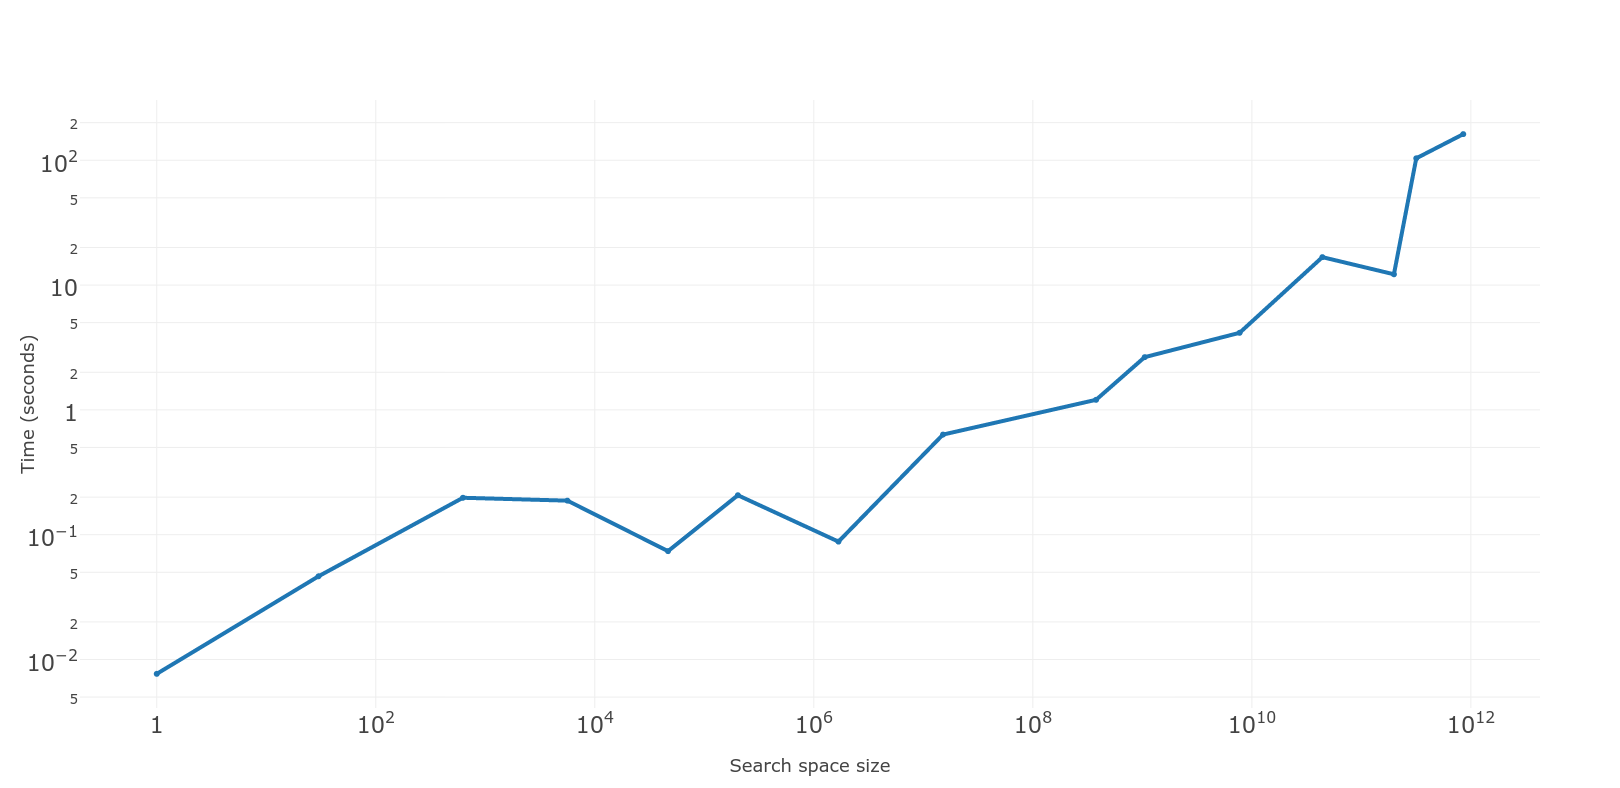
\includegraphics[width=\columnwidth]{plot-sec-mult-no-labels.png}
\label{fig:plot-sec-mult}
\caption{Running times for satisfiable and unsatisfiable variants of 
the secure multiplication sketch.}
\end{figure}


\subsection{Du-Atallah Secure Multiplication}

Similar to the example in Sec.~\ref{sec:ex}, 
Alice and Bob wish to carry out secure multiplication of 
their values (\texttt{input(A)}, \texttt{input(B)} $\in \mathbb{Z}_q$),
with the help of Carol who distributes random values to both the parties.
The only difference now is that the functional requirement now specifies
that the sum of the shares computed by Alice, Bob 
and Carol equals the product of the initial values 
that Alice and Bob had access to.
That is, if \texttt{output(A)}, \texttt{output(B)} and \texttt{output(C)}
respectively represent the shares computed by Alice, Bob and Carol, then
$$
\mathtt{output(A)} + \mathtt{output(B)} + \mathtt{output(C)} = \mathtt{input(A)}*\mathtt{input(B)}.
$$
As before, none of the public announcements should reveal anything
about individual shares.

By slightly modifying the sketch from the illustrative example 
(Sec.~\ref{sec:ex}) we discovered the following 
protocol, which resembles the previously known Du-Atallah protocol~\cite{DA01} :

\begin{enumerate}
    \item Carol generates two random numbers : $x$ which it forwards to Alice
        and $y$ which it forwards to Bob.
    \item Alice computes $\mathtt{input(A)} + x$ and sends to Bob,
        and Bob computes $\mathtt{input(B)} + y$ and sends to Alice.
    \item Alice, Bob and Carol announce $-x\times(y+b)$, $b\times(x+a)$ and 
        $x\times y$ as their shares.
\end{enumerate}

\subsection{Dining Cryptographers}

Anonimity protocols such as the Dining Cryptographers protocol,
proposed by Chaum~\cite{Chaum88}, are an interesting class of protocols for secure
multi-party computation.
The Dining Cryptographers' problem involves 3 cryptographers who decide to
dine-in together. The restaurant allows for anonymous payment of the bill,
which could be paid by, either the National Security Agency (NSA),
or one of the three cryptogtaphers.
The cryptographers respect each other's right to make an anonymous payment, 
but want to find out whether the NSA paid.
The original protocol proposed by Chaum is a two-stage protocol.
In the first stage, every pair of cryptographers establish 
a shared one-bit secret. 
In the second stage, each cryptographer announces 
whether the bits shared with him have
\begin{itemize}
    \item the same parity, if he did not pay the bill.
    \item different parity, if he paid the bill.
\end{itemize}
An odd number of differences are uttered at the table if and only if
one of the cryptographers paid for the dinner (assuming at most 
one of the cryptographers' paid).
The protocol ensures that if a cryptographer is paying, 
neither of the other two learns anything about who made the payment, 
by observing the announcements.

The components used for the sketch are boolean operations such as \texttt{and},
\texttt{or}, \texttt{xor} and \texttt{not}, and random generators \texttt{genAB},
\texttt{genBC} and \texttt{genCA}.
One way to express the functional requirement for the protocol is to 
express the semantics and the correctness criteria in the domain of boolean variables,
thus using the primal ($\exists \forall$) paradigm.
Again, the correctness requirement, like in the case of secure 
multiplication (Sec.~\ref{sec:ex}), can also be expressed in the
abstract domain of boolean formulae expessed in Algebraic Normal Form 
(XOR of AND of variables), thus allowing for synthesis using $\exists \exists$
paradigm.
In both cases, the non-functional security requirement
can be expressed in another dual domain where the domain values
maintain the different sources of randomness, 
and interact differently with different logical operations.


\subsection{Oblivious Transfer}

In the two party version of oblivious transfer (OT), 
one party, the \sender, has two messages $m_0$ and $m_1$,
and the other party, the \chooser, can pick which message she wants to receive.
The goal of oblivious transfer is to achieve this transfer of
message from \sender\ to the \chooser, but with the additional
requirements that
(a) the \sender\ does not learn the choice made by the \chooser,
and
(b) the \chooser\ does not learn the content of the other message 
(that was not chosen).

We wish to base the protocol on the decisional Diffie-Hellman (DDH) assumption~\cite{Boneh:DDH}:
given a cyclic group with generator $g$, the DDH assumption states that
$(g^a,g^b,g^{ab})$ is computationally indistinguishable from
$(g^a,g^b,g^c)$ for randomly and independently chosen elements $a,b,c$ from $\mathbb{Z}$.

% Shortening this section
% We first collect the set of primitives that we can use to synthesize an OT protocol.
% In essence,
% (1) each party can pick some random numbers from $\mathbb{Z}$;
% (2) each party can compute $g^x$, $x^y$, $x*y$ and $x/y$ 
 % if they have access to $x$ and $y$, where $g$ is the generator of the cyclic group;
% (3) each party can send values to the other party;
% (4) the \sender\ can use a group element $g^x$ as a key to encrypt (one of the) messages; and
% (5) the \chooser\ can compute a pair $(v_1,v_2)$ of values with the implicit assumption that
% the left value $v_1$ is used by the \chooser\ when she picks $m_0$ and 
% the right value $v_2$ is used by the \chooser\ when she picks $m_1$.

We provide a sketch to the synthesis tool that consists of four blocks of straight-line code.
It is assumed that the \sender\ has access to random and independently chosen elements 
$r,s$ from $\mathbb{Z}$, and the \chooser\ has access random and independently chosen
elements $a,b,c\in\mathbb{Z}$.

%The program sketch says the following:
% Adria: Shortening this section
%% \\
%% (1) In Block 1, the \sender\ can do nothing, or send $y=g^r$ to the \chooser.
%% \\
%% (2) In Block 2, the \chooser\ can compute $v=g^x$ for $x\in\{a,b,c\}$, or compute
%% a pair $(y*v,v)$ or a pair $(v*v',v'')$ or reverse a pre-computed pair, 
%% where $y$ is the value received from the \sender; furthermore,
%% the \chooser\ can send these values to the \sender.
%% When the \chooser\ sends a pair $(v_1,v_2)$ of values to the \sender, 
%% the implicit understanding is that
%% the left value $v_1$ is the value actually sent when the \chooser\ picks $m_0$ and 
%% the right value $v_2$ is the value actually sent when the \chooser\ picks $m_1$.
%% \\
%% (3) In Block 3, the \sender\ can compute new values using operators
%% $x^y$, $x*y$ or $x/y$ if she has access to $x$ and $y$;
%% she then picks 3 values from the 
%% computed set -- a key $k_0$ to
%% encrypt $m_0$, a second key $k_1$ to encrypt $m_1$, and a third value as a helper value
%% to be send to the \chooser.
%% \\
%% (4) In Block 4, the \chooser\ uses exponentiation on known values to extract key $k_0$ or $k_1$.

We are again able to perform synthesis 
by completely eliminating the primal components
and using only suitably designed % The key novelty in our synthesis approach  is that
{\em{dual programs}}.
Thus, we solve the OT synthesis problem by generating 
an $\Phi_{\exists\exists}$ formula, which is then solved using an
off-the-shelf SMT solver~\cite{yices,z3}.
%
The domain $\domd$ of our dual interpretation is just a fixed length
vector of real numbers. 
%For simplicity, say these are length $1$ vectors.
%For random values $r,s,a,b,c\in\mathbb{Z}$, we use fixed prime numbers;
%say $r=83,s=11,a=29,b=71,c=23$. 
When there is a computation of $g^x$, the program {\em{does not}} perform any computation,
but rather just stores $g^x$ as $x$ -- for each value, the program is cognizant of
which party has access to $x$ and which party has access to only $g^x$.
All arithmetic operations on group elements are mapped to arithmetic operations
on the exponents in the obvious way: for example, $(g^x)^y$ is simply $g^{xy}$,
and $g^xg^y$ is simply $g^{x+y}$. 

%We capture the requirements of the OT protocol as follows:
%(a) we ensure that the \chooser\ can extract message $m_0$, when it has picked $m_0$,
%by checking that the (dual) value computed on Block 4 is equal to the key $k_0$
%computed in Block 3;
%(b) we check that the \chooser\ {\em{can not}} extract message $m_1$, when it has picked $m_0$,
%by checking that the key $k_1$ computed in Block 3 is not in the set of values that the
%\chooser\ can compute using some fixed-size expressions (that are explicitly enumerated);
%(c) we check that the \sender\ {\em{can not}} learn the choice made by the \chooser\ by
%checking that the \sender\ is unable to generate the values sent by the \chooser.
%We note that the checks in (b) and~(c) are necessarily incomplete. Nevertheless, they are
%very effective in pruning out obviously insecure protocols.

Using the above approach, we synthesized two different OT protocols:
the first protocol we synthesized was also recently reported in~\cite{SimpleOT},
and the second protocol we synthesized is the Naor-Pinkas oblivious transfer protocol~\cite{Pinkas}.
The solutions were obtained in $\tilde 1$ and $\tilde 100$ seconds in a regular laptop, 
using Yices as a backend solver.

%\begin{remark}
Because of the approximations involved in capturing the security
property, in this case
%in some cases, in our applications of synthesis to security, 
there is 
%often 
a need for {\em{a posteriori}} verification of security 
of the synthesized scheme using other dedicated verification tools; 
such as, Easycrypt~\cite{easycrypt}. 
However, the program synthesis tool is a fast and effective tool to 
quickly generate plausible schemes.
%\end{remark}

% Adria The data in this section is now distributed in previus sections 
%% 
\begin{table}[t]
\begin{center}
\begin{tabular}{||l|c|c|c|c|c||}
  \hline
  Name & LoC & $|\Sig|$ & P{\small{rimal}} & D{\small{ual}} & T{\small{ime (s)}}
  \\
  \hline
  Simple OT & 9 & 11 & No & Yes & $\sim 1$
  \\
  Naor-Pinkas OT & 16 & 11 & No & Yes & $\sim 100$
  \\
  Padding schemes & 12 & 5 & Yes & Yes & $\sim 1$
  \\
  Padding schemes & 8 & 5 & No & Yes & $\sim 1$
  \\
  BC Modes & 19 & 7 & Yes & Yes & $\sim 10$
  \\
  BC Modes & 24 & 7 & Yes & Yes & $\sim 100$
  \\
  BC Modes & 14 & 7 & No & Yes & $\sim 1$
  \\
  BC Modes & 19 & 7 & No & Yes & $\sim 1$
  \\ \hline
\end{tabular}
\end{center}
\caption{{\small{Synthesis with Duality: Various variants of padding schemes, block cipher modes,
and oblivious transfer were synthesized. The table shows the number of lines synthesized
({\tt{LoC}}),
the number of function symbols given to the synthesizer (${\mathtt{|\Sig|}}$), 
order of magnitude time taken to perform synthesis ({\tt{Time}}), and whether
primal ({\tt{Primal}}) and dual ({\tt{Dual}}) semantics were used.}}}
\label{table}
\end{table}




%% \subsection{Experimental Results}

%% \begin{figure}
%% \centering
%% \begin{tikzpicture}
%%   %\useasboundingbox (-1,-1) rectangle (11,11); 
%%   \tikzset{DataStyle/.style = {draw=black, thick, shape=circle, inner sep=2pt, text=black}}
%%   \tikzset{OpStyle/.style = {draw=black, thick, shape=rectangle, inner sep=3pt, text=black}}
%%   \tikzset{EdgeStyle/.style   = {thick, ->, >=stealth, shorten <=0pt, shorten >=0pt}}
%%   \tikzset{PortEdgeStyle/.style   = {thick, ->, >=stealth, shorten <=0pt, shorten >=0pt}}


%%   \node(1)[DataStyle]{$C$};
%%   \node(2)[DataStyle, below left=of 1]{$A$};
%%   \node(3)[DataStyle, below right=of 1]{$B$};
%%   \node(4)[left=of 2, xshift=10pt]{{\small $\mathtt{input}(A)$}};
%%   \node(5)[right=of 3, xshift=-10pt]{{\small$\mathtt{input}(B)$}};
%%   \node(6)[below=of 2]{{\small $\mathtt{output}(A)$}};
%%   \node(7)[below=of 3]{{\small $\mathtt{output}(B)$}};
  
%%      \draw[EdgeStyle](1) to node[above left]{$(v_1, v_2)$} (2);
%%      \draw[EdgeStyle](1) to node[above right]{$(v_3, v_4)$} (3);
%%      \draw[EdgeStyle, bend left](2) to node[below]{$(v_5, v_6)$} (3);
%%      \draw[EdgeStyle, bend left](3) to node[below]{$(v_7, v_8)$} (2);
%%       \draw[EdgeStyle](4) to node{} (2);
%%       \draw[EdgeStyle](5) to node{} (3);
%%       \draw[EdgeStyle](2) to node{} (6);
%%       \draw[EdgeStyle](3) to node{} (7);




%% Table~\ref{table} presents some statistics on our effort to synthesize 
%% several different protocols for the above three problems. 
%% For oblivious tranfer (OT), the approach based on using both primal and dual
%% semantics (the $\Psi_{\exists\forall}$ approach) failed, but we were 
%% successful in synthesizing OT protocols by replacing the primal by a dual and
%% using the $\Phi_{\exists\exists}$ approach. 
%% For padding schemes, we could use both approaches, but since the synthesis process
%% is fast, the difference is not significant.
%% For block cipher modes, we could again use both approaches, but when we replaced
%% primal checks by new dual interpretations, synthesis times improved by an order
%% of magnitude.  
%% The results provide evidence that duality is useful: first, without dual
%% semantics, we could not even specify the security requirements; and second,
%% by replacing a primal by a dual, we improved running times by enabling the
%% use of much faster SMT solvers, rather than
%% the slower $\exists\forall$ solvers, at the backend.

%% The {\tt{Time}} column in Table~\ref{table} only shows an
%% ``order of magnitude'' number because synthesis timings are very sensitive and
%% variable due to a lot of factors: (i) SMT solvers can get lucky in finding {\em{one}}
%% satisfying solution in some cases, and in other cases, they can be extremely unlucky,
%% and this variance can be observed even when the same problem is
%% posed only slightly differently, and (ii) minor changes in the details of the sketch,
%% for example, which functions can be used on which program blocks, can have a huge
%% impact on running times.


\section{Related Work}

The idea of associating a program with other (different) programs
appears in the form of ``derived programs''~\cite{clt92}
and ``shadow variables''~\cite{DBLP:journals/scp/Morgan09}.
The associated programs get primal semantics; that is, they
compute just like regular programs, but carry more information, akin to
having multiple primals in our setting.
% Our framework also allows us to do the same, but it also allows
% us to have values that are manipulated in the dual semantics.

Dual programs are not abstract interpreters. In abstract interpretation~\cite{CousotCousot77:POPL},
assertion checking is still a ``forall'' check (just over abstract values) and performed
often using (least) fixpoint style computation,
whereas dual assertion checking is an ``exists'' check and is often performed directly
by solving constraints.  One could encode the existence of an abstract fixpoint as a 
dual program.  Verification using duality can be viewed as a  generalization of the 
constraint-based approach for verification.  We also note that dual programs
can be written that are completely unrelated to their primal counterparts.
In fact, often properties related to security, such as
secure information flow~\cite{DBLP:journals/cacm/DenningD77,DBLP:journals/jsac/SabelfeldM03},
are tested by designing 
dedicated ``type systems'' that are unrelated
to the concrete semantics~\cite{DBLP:conf/csfw/Smith01,DBLP:conf/csfw/MalozemoffKG14}.
These are ideally captured in dual programs.

Program synthesis has a long history and early work by Manna and Waldinger on
deductive (theorem proving) synthesis~\cite{Manna71} was followed by more recent
work on inductive synthesis, where programs
are not deduced, but synthesized iteratively by finding programs that work correctly on an ever-increasing
input space.  This search is performed using powerful constraint solvers, 
typically, Boolean Satisfiability solvers (SAT) and Satisfiability Modulo Theory solver (SMT).
Apart from the inductive search technique, there are two other important aspects of the
program synthesis problem that has rejuvenated interest in it.  First, the high-level description
of the program intent need not be formal specification. It could be 
an unoptimized program, or a set of input-output examples, or an incomplete specification~\cite{icse10}.  
Second, the search space for programs need not be the set of 
all valid programs.  It can be restricted by specifying
a small set of user-defined primitives (component-based program synthesis), 
giving syntactic restrictions or templates~\cite{DBLP:conf/fmcad/AlurBJMRSSSTU13,Solar05,Solar06,bitvector}.
% For example, imperative programs can be obtained from a given sketch,
% as long as their intended behavior is also
% provided~\cite{DBLP:journals/sttt/Solar-Lezama13}; efficient bitvector
% manipulations can be synthesized from na\"{\i}ve
% implementations~\cite{bitvector}; agent behavior in
% distributed algorithms can be synthesized from a description of a
% global goal~\cite{DBLP:conf/nfm/GasconT14};
% circuits can be repaired
% given a specification of their intended
% behavior~\cite{DBLP:conf/iccad/FujitaJOM13};
% and
% deobfuscated code can be
% obtained using similar ideas~\cite{icse10}. Although
% all these applications rely on template-based synthesis, different
% synthesis algorithms are used in different domains.
Logically, most of the synthesis algorithms are solving
an $\exists\forall$ problem.
Synthesis using duality is a principled way to reduce synthesis to an
$\exists\exists$ problem, and it subsumes both
grammar-based syntactic pruning of program search space,
as well as, type-based pruning~\cite{DBLP:conf/pldi/OseraZ15} of synthesis search space (and more).
% The main challenge in program synthesis is to efficiently reduce the
% synthesis search space. Syntax-guided synthesis (SyGuS) uses syntactic
% constraints to prune the synthesis search space~\cite{DBLP:conf/fmcad/AlurBJMRSSSTU13}.
% These syntactic restrictions are presented as a grammar: the strings generated
% by the grammar forms the synthesis search space.
% There is also work on using type constraints to control the explosion in
% the synthesis search space~\cite{DBLP:conf/pldi/OseraZ15}.
% Synthesis using multiple primal and dual semantics 
% % Primal and dual interpretations 
% is a more general concept that 

Our work builds upon the recent work on synthesis of security schemes
using program synthesis techniques~\cite{TGD15:CADE}, where security
requirements are captured using constraints.
The work described in~\cite{TGD15:CADE} falls in the $\Psi_{\exists\forall}$
paradigm. Here, we introduce duality and use the resulting 
$\Phi_{\exists\exists}$ paradigm for synthesis.
% is focused on the synthesis
% application, and it does not formally present
% and contrast primal and dual semantics.
% Moreover, the work in~\cite{TGD15:CADE} is restricted to
% straight-line programs.

It has been pointed out in~\cite{DBLP:conf/tldi/MarinoM09}
that there are some general principles that govern multiple
specialized type systems; specifically, it is shown that
some standard effect systems can be described uniformly as
granting and checking privileges.
Dual programs can also capture generic rules that
govern the update of attributes, and generation of
constraints. One key observation here is that
dual programs can be written that carry path information;
for example, by having 
a dual variable corresponding to every control flow fork, such
as conditionals, try, and synchronized.
%(such as in
%a conditional statement) maps to stack push.
%Other control flow constructs, such as
%$\mathtt{try}$ and $\mathtt{synchronized}$,
%behave similarly to fork in dual programs.
It is at these special control flow points that
privileges are granted~\cite{DBLP:conf/tldi/MarinoM09,DBLP:journals/toplas/AbadiFF06}, 
which can be captured in dual programs by 
assigning values to these special dual variables.
% (certain ``privileges'') onto the stack.
%Unlike most other work, we do not focus here on
%rules for type checking or reconstruction, but rather
%we just formulate (and generate) ``well-typedness''
%constraints (for the dual semantics) and pass them
%to an SMT, or an $\exists\forall$ SMT, solver.

There is an intriguing connection between our notion of duality 
and query answering in incomplete databases. 
The standard way of answering queries over incomplete
databases is by computing {\em certain answers}, i.e.\ 
query answers that hold {\em for every} possible instance
of the incomplete database. In~\cite{Libkin14},
it has been shown that, with a proper choice of semantics,
computation of certain answers can often we reduced 
to just evaluation. 
Moreover, since computing certain answers is co-NP
for commonly considered semantics, alternate semantics
that provide underapproximations have been also proposed~\cite{Libkin15}.

%Recently, we have implemented an exists-forall solver as part of the
%SMT-solver Yices~\cite{Dutertre:cav2014,DBLP:conf/fmcad/GasconSDTJM14}. In this paper,
%we present a language for specifying sketches, which are partially
%specified programs, but unlike any previous work on synthesis, we use
%two different interpretations for the program symbols. We perform
%synthesis by explicitly generating an exists-forall formula in Yices
%syntax and then use Yices to solve it.

%The component-based program synthesis problem was formulated
%in~\cite{bitvector}, but the interest in~\cite{bitvector} was only
%on functional requirements. Here, we also consider nonfunctional
%requirements, which forces us to reason with two different semantics
%of the same program.
%We use benchmarks from~\cite{bitvector} in this paper.

%The idea of attaching dual semantics to a program
%shares some features with
%the integration of constraints in programming
%languages, as in constraint logic programming.


%dual Our work is also related to the
%constraint logic programming
 %imposes constraints as execution proceeds;
 %variables in constraints are existentially quantified...

%multiple attributes - each with domain, super attr = product of smaller domains

%attributes with variables - two kinds



% prgm = primal + primal + primal + dual + dual ...

% application: synthesis


% Related work--
% Success Typing javascript

\section{Conclusion}

We formulated the notion of
programming with primal and dual components.
The primal component is used to define 
functional correctness, while the dual 
can be used to define nonfunctional properties, 
or perform abstract analysis on the primal.
%The description of the alternate semantics is kept
%separate from the main program.
%Each alternate semantics can be a primal semantics
%or a dual semantics, and we define these two concepts
%in the paper.
When the latter is possible, we get a weak duality principle
whereby we can replace an desired $\forall$ check
by a stronger $\exists$
check.
%In some cases, a it is possible to design dual semantics
%that subsume requirements on a primal semantics; and thus,
%make the primal semantics redundant.
%
This duality principle can speed up 
program synthesis, and we demonstrated this on 
synthesis of cryptographic schemes.

%\acks
%
%Acknowledgments, if needed.

% We recommend abbrvnat bibliography style.



%\bibliographystyle{plain}
%\bibliographystyle{abbrvnat}
\bibliographystyle{abbrv}
\bibliography{all}

\ignore{

\appendix
\section{Proof Sketches of Main Claims}
\begin{theorem} [Theorem~\ref{thm:duality}]
  Let $P$ be a program in static single assignment form
  and $\gamma$ satisfies the Cartesian assumption.
  Let $U\subseteq \psp$ be a set of primal initial states,
  and let $U'\subseteq\psd$ be such that
  $U|_{\V_1} \subseteq \gamma(\ds)|_{\V_1}$ for every $\ds\in U'$.
  If $\semd$ is an abstraction of $\semp$,
  then
  $\semp(P)(U) \subseteq \gamma(\ds)$ for every $\ds\in\semd(P)(U'))$.
\end{theorem}
\begin{proof}(Sketch)
  Let $\sigma\in\semp(P)(U)$.
  By definition (Equation~\ref{eqn:primalProgram}),
  it follows that there exists a path $\pi\in\paths(v_s,v_e)$
  such that $\sigma\in \semp(\pi)(U)$.
  %Let $l(\pi) = s_1;s_2;\ldots;s_k$.
  We need to prove that $\sigma\in\gamma(\ds)$ for every $\ds\in\semd(P)(U'))$.
  By definition of $\semd$ for programs, % (Equation~\ref{eqn:dualProgram}),
  we need to prove that $\sigma\in\gamma(\ds)$ for every $\ds\in (U'\cap \bigcap_i \semd(e_i))$,
  where $e_i$'s are program edges.

  Recall that 
  the sets $\V_1,\ldots,\V_m$ are disjoint; and moreover,
  the variables $\V_i$ are defined on paths $\pi\in\paths(v_s,v_e)$.
% while the rest are undefined.
  %Let $W_i = \V_1\cup\cdots\cup\V_i$ be the set of all primal program variables
  %that are updated in the first on paths up to the essential node $v_i$.
  %Let $K_i = L_1\cup\cdots\cup L_i$ be the set of dual variables corresponding to
  %program locations in the part of the program between the essential
  %nodes $v_{i-1}$ and $v_i$.
%
  Consider an arbitrary dual state $\ds$ in $(U'\cap \bigcap_i \semd(e_i))$.
  We need to prove that $\sigma\in\gamma(\ds)$.
  We prove that
  the projection of $\sigma$ onto the
  variables $W_i = \V_1\cup\cdots\cup \V_i$, namely
  $\sigma|_{W_i}$, is in the set $\gamma(\ds)|_{W_i}$.
  We prove this by induction on $i$.
  For the base case $i=1$, $W_1=\V_1$. Recall that $\V_1$
  is the set of input variables. Since input variables
  are not updated later by $P$, we have
  $\sigma|_{W_1}=U|_{\V_1}$, and by assumption,
  this is contained in the set $\gamma(\ds)|_{W_1}$ for every
  $\ds\in U'$. But, we know that $\ds\in U'$ and this establishes
  the base case. %$\gamma(\ds)|_{W_i}$.

  For the induction step, % Suppose not. Then, there is minimal $i$ such that
  % the projection of $\sigma$ onto the
  % variables $W_i = \V_1\cup\cdots\cup \V_i$, namely
  % $\sigma|_{W_i}$, is not in the set $\gamma(\ds)|_{W_i}$.
  % By minimality of $i$,
  we can assume
  $\sigma|_{W_{i-1}}$ is in the set $\gamma(\ds)|_{W_{i-1}}$.
  But, we know that $\ds\in \semd(e_i)$ for every edge in $\paths(v_s,v_i)$.
  Therefore, since the ``inputs'' $W_{i-1}$ satisfy the precondition,
  we know that the ``outputs'' $\V_i$ satisfy the postcondition of $\gamma(\ds)$.
  % $\sigma|_{W_{i-1}}$ is in the set $\gamma(\ds)|_{W_{i-1}}$.
  That is, from the definition of abstraction,
  we have $\sigma|_{\V_i} \in \gamma(\ds)|_{\V_i}$.
  Since we assumed that $\gamma$ satisfies the Cartesian condition,
  it follows that
  we have $\sigma|_{W_i} \in \gamma(\ds)|_{W_i})$.
\end{proof}

\begin{corollary}\label{cor:duality}
  Let $l\approx d$ be a dual assertion and $x=c$ be a primal assertion
  such that $\gamma(\{\sigma \mid \sigma(l)=d\}) \subseteq \{\sigma \mid \sigma(x)=c\}$.
  If the dual is an abstraction of the primal (as in Theorem~\ref{thm:duality}),
  then, whenever
  $l \approx d$ holds in $P$ in the dual semantics, then
  $x = c$ holds in $P$ in the primal semantics.
\end{corollary}
\begin{proof}
  Let $\ds\in\semt(P)(U')$.
  Since $l\approx d$ holds in $P$ in the dual semantics,
  it follows that $\ds(l)=d$.
  Let $\sigma\in\sem(P)(U)$ be any reachable primal state.
  We need to show that $\sigma(x)=c$.
  Since the dual semantics is an abstraction of the primal,
  it follows from Theorem~\ref{thm:duality} that
  $\sigma\in\gamma(\ds)$.
  Since we assumed that
  $\gamma(\{\sigma \mid \sigma(l)=d\}) \subseteq \{\sigma \mid \sigma(x)=c\}$,
  and since $\ds(l)=d$,
  it follows that
  $\gamma(\ds) \subseteq \{\sigma \mid \sigma(x)=c\}$.
  Since $\sigma\in\gamma(\ds)$,
  it follows that $\sigma\in \{\sigma \mid \sigma(x)=c\}$,
  which implies $\sigma(x)=c$.
\end{proof}
\endignore}

\end{document}
